\documentclass[oneside]{book}

\setcounter{tocdepth}{2}
\setcounter{secnumdepth}{3}

\usepackage[toc,page]{appendix}
\usepackage{minted}
\usepackage[english]{babel}
\usepackage{graphicx}
\usepackage{hyperref}
\usepackage{amsmath} % Required for some math elements 
\usepackage{pdflscape}
\usepackage{pdfpages}
\usepackage{float}
\usepackage{subcaption}
\usepackage{verbatim}
\usepackage{epigraph}
\usepackage{titlesec}
\usepackage{multirow}
\usepackage[]{algorithm2e}

\interfootnotelinepenalty=10000

\newminted[HaskellCode]{haskell}{fontsize=\footnotesize}

\makeatletter
\titleformat{\part}[display]
  {\Huge\scshape\filright}
  {\partname~\thepart:}
  {20pt}
  {\thispagestyle{epigraph}}
\makeatother
\setlength\epigraphwidth{.6\textwidth}

\begin{document}

\begin{titlepage}
	\centering
	
\includegraphics[width=0.60\textwidth]{./logo/UoN_Primary_Logo_RGB.png}\par\vspace{1cm}
	{\scshape\Large PhD Thesis\par}
	\vspace{1.5cm}
	%{\huge\bfseries Foundations Of Pure Functional \\ Agent-Based Simulation \par}
%	{\huge\bfseries Pure Functional Programming \\ In Agent-Based Simulation \par}
	{\huge\bfseries The Pure Functional Programming Paradigm \\ In Agent-Based Simulation \par}
	\vspace{2cm}
	{\Large Jonathan Thaler (4276122) \\ \itshape jonathan.thaler@nottingham.ac.uk \par}
	\vfill
	supervised by\par
	Dr. Peer-Olaf \textsc{Siebers} \\
	Dr. Thorsten \textsc{Altenkirch}

	\vfill

	{\large \today\par}
\end{titlepage}

\cleardoublepage

\section*{Abstract}
This thesis shows how to implement Agent-Based Simulations (ABS) using the \textit{pure} functional programming paradigm and what the benefits and drawbacks are when doing so. As language of choice, Haskell is used due to its modern nature, increasing use in real-world applications and \textit{pure} nature. The thesis presents various implementation techniques to ABS and then discusses concurrency and parallelism and verification and validation in ABS in a pure functional setting. Additionally the thesis briefly discusses the use of dependent types in ABS, to close the gap between specification and implementation - something the presented implementation techniques don't focus on.
Finally a case-study is presented which tries to bring together the insights of the previous chapters by replicating an agent-based model both in pure and dependently typed functional programming. The agent-based model which was selected was much discussed in ABS communities as it claimed to have solved a fundamental problem of economics but it was then found that the implementation had a number of bugs which shed doubt on the validity and correctness of the results. The thesis' case study investigates whether this failure could have happened in pure and dependent functional programming and is a further test to see of how much value functional programming is to ABS. \\

TODO "finalise research" milestone until end of June 2019
\begin{enumerate}
	\item finish property-base testing work in Haskell: make sense of the SIR model verification which does not work: either give an in-depth explanation why not and why our implementation is still valid or find a way of solving it.

	\item implement SIR equilibrium-totality correspondence in Idris, closely related to the property-based testing

	\item implement Gintis Case-Study and focus on property-tests and reasoning and potential directions for a dependently-typed implementation. this will be highly important for my internal assessor 
\end{enumerate}

TODO "first draft" milestone until end of July 2019
\begin{enumerate}
	\item Revise and finalise methodology.

	\item Write short monad transformer section in methodology

	\item Draft all chapters of discussion part.
	
	\item Write a first draft of conclusions and future research
\end{enumerate}

TODO "reflecting and filling in holes" milestone until end of August 2019
\begin{enumerate}
	\item Reading: Ionescu thesis
	
	\item Understand Ionescu: check what ionescou wants from his students and what literaure he cites, watch YouTube video

	\item Generalising ABS: extract the foundational properties: agents as monad / comonad / arrow and discuss their implications from an abstract point of view
	
	\item Refine Presentation: Has to come across as a thesis, not a technical report! Need to discuss concepts more generally and derive more concepts from the explanations, otherwise it looks like an advanced technical report.
\end{enumerate}

TODO "cleaning up / polishing" milestone until beginning of September 2019
\begin{enumerate}
	\item consistency of words / expressions
		\begin{itemize}
			\item s vs 's vs. s' e.g. Agents vs. Agents's vs. Agents'
			\item case study vs. case-study (no -)
			\item Monad vs monad (lower/upper case?)
			\item speedup vs speed up vs speed-up
			\item types / function names / monad names ITALIC!?
			\item main-thread vs main thread
			\item avoid don't, won't, haven't, e.g.,... and write them all out
		\end{itemize}
	\item proof reading

	\item refining expressions
	
	\item reconcile all code into thesis code folder?
	
	\item extract all references of the thesis in separate file and manually fine-tune them so that they are perfect: including DOI, include link to webpage in case of a blog,...
	
	\item PERFECT introduction chapter
	
	\item PERFECT conclusion chapter
\end{enumerate}

TODO prepare for viva:
\begin{enumerate}
	\item read transformers chapters
	
	\item read exception chapter

	\item read basic libraries chapter	
	
	\item completely understand monad-transformers: what is executed in which order? what about commutativity? e.g. STM is innermost monad, will be evaluated last to get an IO but this in fact leads then to the evaluation of all the monads before because STM is able to re-run
\end{enumerate}

%TODO: from the 2nd annual review i got the feedback that i need to come up with a more coherent thesis structure which tells a story: i need to make myself clear what story i want to tell with my phd and what research and publications i still need to do for that (identify chapters and to which extent they are already finished). Also I need to come up with a precise publication plan, focusing on writing papers early than doing research for a too long time and starting an early thesis writing. This is because any unpublished research is lost and every published research is a contribution to knowledge. "A good PhD is asking more questions than it answers."

\clearpage
\tableofcontents
\clearpage
\textit{To my parents for their unconditional love and support throughout all my life.}
\clearpage

\chapter*{Acknowledgements}
Peer-Olaf Siebers Supervisor
Thorsten Altenkirch Supervisor
FP Group, for always being open to discussions, keen to help.
Martin Handley and James Hey for working through my thesis and their feedback.
Ivan Perez for always having an open ear for questions, valuable discussions with him and his contributions.
Julie Greensmith for the valuable discussions and pointing me into right directions at important stages of the phd.

% PART I: Beginnings
\epigraphhead[450]{}
\part{Preliminiaries}

\section{Introduction}
There exists a large number of simulation packages which allow the convenient creation of System Dynamics simulations by straight-forward visual diagram creation. One simply creates stocks and flows, connects them, specifies the flow-rates and initial parameters and then runs the model. An example for such a visual diagram creation in the simulation package AnyLogic can be seen in Figure \ref{fig:sir_stockflow_diagram}.

\begin{figure}
	\centering
	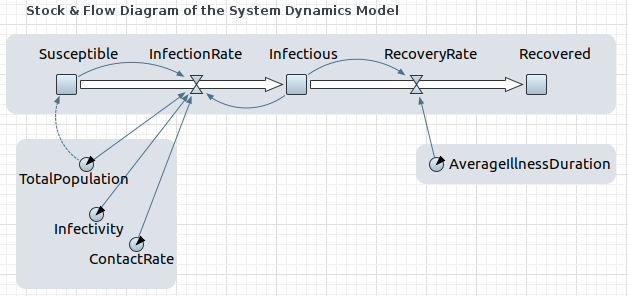
\includegraphics[width=.5\textwidth, angle=0]{./fig/SIR_SD_STOCKFLOW_DIAGRAMM.png}
	\caption{Visual System Dynamics Diagram of the SIR model in AnyLogic Personal Learning Edition 8.3.1.}
	\label{fig:sir_stockflow_diagram}
\end{figure}

Still, implementing System Dynamics directly in code is not as straight forward and involves numerical integration which can be quite tricky to get right. Thus, the aim of this paper is to look into how System Dynamics models can be implemented in code correctly without the use of a simulation package. We use the well known SIR model \cite{kermack_contribution_1927} from epidemiology to demonstrate our approach.

Our language of choice is Haskell because it emphasises a declarative programming style in which one describes \textit{what} instead of \textit{how} to compute. Further it allows to rule out interference with non-deterministic influences or side-effects already at compile-time. This is of fundamental importance for System Dynamics because it behaves completely deterministic and involves no stochastics or non-determinism whatsoever. Also, we make use of Functional Reactive Programming which allows to express continuous-time systems in a functional way. 

We show that by this approach we can arrive at correct-by-construction implementations of System Dynamic models. This means that the correctness of the code is obvious because we have closed the gap between the model specification and its implementation. Thus, the contribution of the paper is the demonstration of how to implement correct-by-construction System Dynamics simulations using Haskell and Functional Reactive Programming.

\section{Related research and literature}
\label{sec:literature}

The amount of research on using pure functional programming with Haskell in the field of ABS has been moderate so far. Most of the papers are related to the field of Multi Agent Systems (MAS) and look into how agents can be specified using the belief-desire-intention paradigm \cite{de_jong_suitability_2014,sulzmann_specifying_2007,jankovic_functional_2007}.

A multi-method simulation library in Haskell called \textit{Aivika 3} is described in the technical report \cite{sorokin_aivika_2015}. It supports implementing Discrete Event Simulations (DES), System Dynamics and comes with basic features for event-driven ABS which is realised using DES under the hood. Further it provides functionality for adding GPSS to models and supports parallel and distributed simulations. It runs within the IO effect type for realising parallel and distributed simulation but also discusses generalising their approach to avoid running in IO.

In his master thesis \cite{bezirgiannis_improving_2013} the author investigates Haskells' parallel and concurrency features to implement (amongst others) \textit{HLogo}, a Haskell clone of the NetLogo \cite{wilensky_introduction_2015} simulation package, focusing on using STM for a limited form of agent-interactions. \textit{HLogo} is basically a re-implementation of NetLogos API in Haskell where agents run within the IO context and thus can also make use of STM functionality. The benchmarks show that this approach does indeed result in a speed-up especially under larger agent-populations. The authors' thesis is one of the first on ABS using Haskell. Despite the concurrency and parallel aspect, this thesis approach is rather different: it avoids IO within the agents under all costs and explore the use of STM more on a conceptual level rather than implementing an ABS library to compare our case-studies with lock-based and imperative implementations.

There exists some research \cite{di_stefano_using_2005, varela_modelling_2004, sher_agent-based_2013} using the functional programming language Erlang \cite{armstrong_erlang_2010} to implement concurrent ABS. The language is inspired by the actor model \cite{agha_actors:_1986} and was created in 1986 by Joe Armstrong for Eriksson for developing distributed high reliability software in telecommunications. The actor model can be seen as quite influential to the development of the concept of agents in ABS, which borrowed it from Multi Agent Systems \cite{wooldridge_introduction_2009}. It emphasises message-passing concurrency with share-nothing semantics (no shared state between agents), which maps nicely to functional programming concepts. The mentioned papers investigate how the actor model can be used to close the conceptual gap between agent-specifications, which focus on message-passing and their implementation. Further they show that using this kind of concurrency allows to overcome some problems of low level concurrent programming as well.
Also \cite{bezirgiannis_improving_2013} ported NetLogos API to Erlang mapping agents to concurrently running processes, which interact with each other by message-passing. With some restrictions on the agent-interactions this model worked, which shows that using concurrent message-passing for parallel ABS is at least \textit{conceptually} feasible. Despite the natural mapping of ABS concepts to such an actor language, it leads to simulations, which despite same initial starting conditions, might result in different dynamics each time due to concurrency.

The work \cite{lysenko_framework_2008} discusses a framework, which allows to map Agent-Based Simulations to Graphics Processing Units (GPU). Amongst others they use the SugarScape model \cite{epstein_growing_1996} and scale it up to millions of agents on very large environment grids. They reported an impressive speed-up of a factor of 9,000. Although their work is conceptually very different this thesis draws inspiration from their work in terms of performance measurement and comparison to the Sugarscape model.

% THIS IS MY OWN REASEARCH, DON'T CITE IT HERE
%In \cite{thaler_pure_2019} the authors showed how to implement a spatial SIR model in pure Haskell using Functional Reactive Programming \cite{hudak_arrows_2003}. They report quite low performance but mention that STM may be a way to considerably speed up the simulation. We follow their approach in implementation technique, using Functional Reactive Programming and Monadic Stream Functions \cite{perez_functional_2016} (we don't go into implementation details as it is out of the scope of this paper) and use the spatial SIR model as the first case-study.

Using functional programming for DES was discussed in \cite{jankovic_functional_2007} where the authors explicitly mention the paradigm of Functional Reactive Programming (FRP) to be very suitable to DES.

A domain-specific language for developing functional reactive agent-based simulations was presented in \cite{schneider_towards_2012,vendrov_frabjous_2014}. This language called FRABJOUS is human readable and easily understandable by domain-experts. It is not directly implemented in FRP/Haskell but is compiled to Haskell code which they claim is also readable. This supports that FRP is a suitable approach to implement ABS in Haskell. Unfortunately, the authors do not discuss their mapping of ABS to FRP on a technical level, which would be of most interest to functional programmers.

Object-oriented programming and simulation have a long history together as the former one emereged out of Simula 67 \cite{dahl_birth_2002}, which was created for simulation purposes. Simula 67 already supported DES and was highly influential for today's object-oriented languages. Although the language was important and influential, in our research we look into different approaches, orthogonal to the existing object-oriented concepts.

Lustre is a formally defined, declarative and synchronous dataflow programming language for programming reactive systems \cite{halbwachs_synchronous_1991}. While it has solved some issues related to implementing ABS in Haskell, it still lacks a few important features necessary for ABS. There seems to be no way of implementing an environment in Lustre as it is done in Chapters \ref{ch:timedriven} and \ref{ch:eventdriven}. Also, the language seems not to come with stochastic functions, which are but the very building blocks of ABS. Finally, Lustre does only support static networks, which is clearly a drawback in ABS in general where agents can be created and terminated dynamically during simulation.

In \cite{botta_time_2010}, the authors discuss the problem of advancing time in message-driven agent-based socio-economic models. They formulate purely functional definitions for agents and their interactions through messages. Our architecture for synchronous agent-interaction as discussed in Chapter \ref{sec:eventdriven_implementation} was not directly inspired by their work but has some similarities: the use of messages and the problem of when to advance time in models which allows unrestricted synchronised agent interactions.

The authors of \cite{botta_functional_2011} are using functional programming as a specification for an agent-based model of exchange markets but leave the implementation for further research where they claim that it requires dependent types. This paper is the closest usage of dependent types in agent-based simulation we could find in the existing literature and to our best knowledge there exists no work on general concepts of implementing pure functional agent-based simulations with dependent types. %As a remedy to having no related work to build on, we looked into works which apply dependent types to solve real world problems from which we then can draw inspiration from.

In his talk \cite{sweeney_next_2006}, Tim Sweeney CTO of Epic Games discussed programming languages in the development of game engines and scripting of game logic. Although the fields of games and ABS seem to be very different, Gregory \cite{gregory_game_2018} defines computer-games as \textit{"[..] soft real-time interactive agent-based computer simulations"} (p. 9) and indeed, they have striking similarities: both are simulations which perform numerical computations and update objects in a loop either concurrently or sequential. In games these objects are called \textit{game-objects} and in ABS they are called \textit{agents} but they are conceptually the same thing.  Sweeney reports that reliability suffers from dynamic failure in languages like C++ e.g. random memory overwrites, memory leaks, accessing arrays out-of-bounds, dereferencing null pointers, integer overflow, accessing uninitialized variables. He reports that 50\% of all bugs in the Game Engine Middleware Unreal can be traced back to such problems and presents dependent types as a potential rescue to those problems. The two main points Sweeney made were that dependent types could solve most of the run-time failures and that parallelism is the future for performance improvement in games. He distinguishes between pure functional algorithms which can be parallelised easily in a pure functional language and updating game-objects concurrently using Software Transactional Memory (STM).

\chapter{Methodology}
This chapter introduces the background and methodology used in the following chapters. Roughly 50\% exists already.

\section{Agent-Based Simulation}
History, methodology (what is the purpose of ABS: 3rd way of doing science: exploratory, helps understand real-world phenomena), classification according to \cite{macal_everything_2016}, ABS vs. MAS, event- vs. time-driven \cite{meyer_event-driven_2014}, examples: agent-based SIR, SugarScape, Gintis Bartering

\subsection{Traditional approaches}
Introduce established implementation approaches to ABS. Frameworks: NetLogo, Anylogic, Libraries: RePast, DesmoJ. Programming: Java, Python, C++. Correctness: ad-hoc, manual testing, test-driven development.

\subsection{Verification \& Validation}
Introduction Verification \& Validation (V \& V in the context of ABS).

%--------------------------------------------------------------------------

\section{Pure functional programming}
Definition, Haskell references,

In our research we are using the \textit{pure} functional programming language Haskell. The paper of \cite{hudak_history_2007} gives a comprehensive overview over the history of the language, how it developed and its features and is very interesting to read and get accustomed to the background of the language. The main points why we decided to go for Haskell are:

\begin{itemize}
	\item Rich Feature-Set - it has all fundamental concepts of the pure functional programming paradigm included. Further, Haskell has influenced a large number of languages, underlining its importance and influence in programming language design.
	\item Real-World applications - the strength of Haskell has been proven through a vast amount of highly diverse real-world applications \cite{hudak_haskell_1994, hudak_history_2007}, is applicable to a number of real-world problems \cite{osullivan_real_2008} and has a large number of libraries available \footnote{\url{https://wiki.haskell.org/Applications_and_libraries}}.
	\item Modern - Haskell is constantly evolving through its community and adapting to keep up with the fast changing field of computer science. Further, the community is the main source of high-quality libraries.
	\item Purity - Haskell is a \textit{pure} functional language and in our research it is absolutely paramount, that we focus on \textit{pure} functional ABS, which avoids any IO type under all circumstances (exceptions are when doing concurrency but there we restrict most of the concepts to STM).
	\item It is as closest to pure functional programming, as in the lambda-calculus, as we want to get. Other languages are often a mix of paradigms and soften some criteria / are not strictly functional and have different purposes. Also Haskell is very strong rooted in Academia and lots of knowledge is available, especially at Nottingham, 
		Lisp / Scheme was considered because it was the very first functional programming language but deemed to be not modern enough with lack of sufficient libraries. Also it would have given the 
		Erlang was considered in prototyping and allows to map the messaging concept of ABS nicely to a concurrent language but was ultimately rejected due to its main focus on concurrency and not being purely functional.
		Scala was considered as well and has been used in the research on the Art Of Iterating paper but is not purely functional and can be also impure.
\end{itemize}


\subsection{Functional Reactive Programming}
Short introduction to FRP (yampa), based on my pure functional epidemics paper.

\subsection{Monadic Stream Functions}
Short introduction to MSFs (dunai), based on my pure functional epidemics paper.

\section{Dependent Types}
Example, Equality as Type, Philosophical Foundations: Constructive mathematics

\section{Implementing ABS}
\label{ch:impl_abs}
In this section we briefly present a general background on problems and considerations, ABS implementations need to solve independent from the programming paradigm. In general, an ABS implementation must solve the following fundamental problems:

\begin{enumerate}
	\item How to represent an agent, its local state and its interface.
	\item How to represent agent-to-agent interactions and enforcing their semantics.
	\item How to represent an environment.
	\item How to represent agent-to-environment interactions and enforcing their semantics.
	\item How agents and an environment can initiate actions without external stimuli.
	\item How to step the simulation.
\end{enumerate}

% agent- and environment pro-activity
We argue that the most fundamental concept of ABS is the \textit{pro-activity} of both, agents and its environment. In computer systems, pro-activity, the ability to initiate actions on its own without external stimuli, is only possible when there is some internal stimulus, most naturally represented by a continuous increasing time-flow. Due to the discrete nature of computer systems, this time-flow must be discretized in steps as well and each step must be made available to the agent, acting as the internal stimulus. This allows the agent then to perceive time and become proactive depending on time. So we can understand an ABS as a discrete time simulation where time is broken down into continuous, real-valued or discrete natural-valued time steps. Independent of the representation of the time-flow we have the two fundamental choices whether the time-flow is local to the agent or whether it is a system-global time-flow. Time-flows in computer systems can only be created through threads of execution where there are two ways of feeding time-flow into an agent. Either it has its own thread-of-execution or the system creates the illusion of its own thread-of-execution by sharing the global thread sequentially among the agents where an agent has to yield the execution back after it has executed its step. %Note the similarity to an operating system with cooperative multitasking in the latter case and real multiprocessing in the former.

% time- and event-driven ABS
Generally, there exist time- and event-driven approaches to ABS \cite{meyer_event-driven_2014}. In time-driven ABS, time is explicitly modelled and is the main driver of the ABS dynamics. The semantics of models using this approach, center around time. As a representative example, which will be used in Chapter \ref{ch:timedriven}, we use the agent-based SIR model \cite{macal_agent-based_2010, thaler_pure_2018}. Often such models are inspired by an underlying System Dynamics approach, where the continuous time-flow is the main driving force of the dynamics. It is clear that almost every ABS models time in some way, after all, modelling a virtual system over some (virtual) time is the very heart of Simulation. Still we want to distinguish clearly between different semantics of time representation in ABS: when time is seen as a continuous flow such as in the example of the agent-based SIR model, we talk about a truly time-driven approach. In other words: if an agent behaves as a time signal then we speak of a time-driven approach. This means that if the system is sampled with a $\Delta t = 0$ then, even though the agents are executed their behaviour must stay constant and must not change.

In the case where time advances in a discrete way either by means of events or messages, we talk about an event-driven approach. As a representative example, which will be used in Chapter \ref{ch:eventdriven} on event-driven ABS, we use an event-driven SIR and the Sugarscape model. In this model time is discrete and represented by the natural numbers where agents act in every tick. In such a model, the underlying semantics map more naturally to a Discrete Event Simulation core, extended by ABS features, as in the event-driven SIR and to a lesser extent in the Sugarscape model.

% agent representation
According to the definition of ABS in  Chapter \ref{sec:method_abs}, an agent is a uniquely addressable entity with an identity, an internal state it has exclusive control over and can be interacted with by means of messages. In the established object-oriented approaches to ABS all this is implemented naturally by the use of objects: an object has a clear identity, encapsulates internal state and exposes an interface through public methods through which objects can interact with each other, also called messaging. The same applies to the environment and it is by no means clear how to achieve this in a pure functional approach where we don't have objects available. This is one of the central questions this thesis is trying to answer and it will be addressed in the subsequent Chapters \ref{ch:timedriven} and \ref{ch:eventdriven}.

Before we look into pure functional ABS implementation concepts in the next chapters, we need to discuss the concept of update strategies \cite{thaler_art_2017}. Generally, there are four strategies to approach time- and event-driven ABS, where the differences deal with how the simulation is stepped, the agents are executed and the interaction semantics work.

% agent-to-agent interaction ant its semantics
%The semantics of messaging define when sent messages are visible to the receivers and when the receivers process them. Message-processing could happen either immediately or delayed, depending on how message-delivery works. There are two ways of message-delivery: immediate or queued. In the case of immediate message-deliver the message is sent directly to the agent without any queuing in between e.g. a direct method-call. This would allow an agent to immediately react to this message as this call of the method transfers the thread-of-execution to the agent. This is not the case in the queued message-delivery where messages are posted to the message-box of an agent and the agent proactively processes the message-box at regular points in time. With established OOP approaches we can have both: either a direct method-call or a message-box approach - in pure functional programming this is a much more subtle problem and it turns out that the problem of messaging / interacting of agents and of agents with the environment is the most subtle problem when approaching ABS from a pure functional perspective.

\subsection{Sequential strategy}
\label{sec:seq_strategy}
In this strategy there exists a globally synchronized time-flow and in each time step the simulation iterates through all the agents and updates one agent after another. Messages sent and changes to the environment made by agents are visible immediately, meaning that if an agent sends messages to other agents or changes the environment, agents which are executed after this agent will see these changes within the same time step. There is no source of randomness and non-determinism, rendering this strategy to be completely deterministic in each step. Messages can be processed either immediately or queued depending on the semantics of the model. If the model requires to process the messages immediately the model must be free of potential infinite-loops. Often in such models, the agents are shuffled when the model semantics require to average out the advantage of being executed as first. This strategy is of fundamental importance for event-driven ABS in Chapter \ref{ch:eventdriven}. See Figure \ref{fig:strategy_seq} for a visualisation of the control flow in this strategy.

\begin{figure}[H]
	\centering
	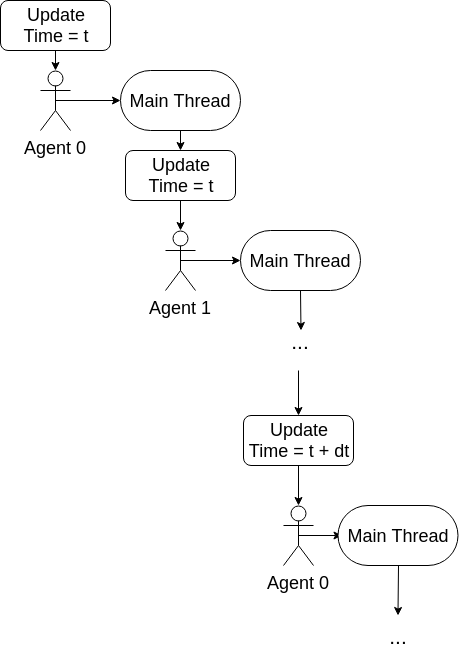
\includegraphics[width=0.5\textwidth, angle=0]{./fig/implabs/sequential.png}
	\caption[Control flow in the sequential update strategy]{Control flow in the sequential update strategy.}
	\label{fig:strategy_seq}
\end{figure}

\subsection{Parallel strategy}
\label{sub:par_strategy}
This strategy has a globally synchronized time-flow and in each time step iterates through all the agents and updates them in parallel. Messages sent and changes to the environment made by agents are visible in the next global step. We can think about this strategy in a way that all agents make their moves at the same time.  If one wants to change the environment in a way that it would be visible to other agents this is regarded as a semantic error in this strategy. First, it is not logical because all actions are meant to happen at the same time and second, it would implicitly induce an ordering, violating the semantics of the model, the \textit{happens at the same time} idea.
It does not make a difference if the agents are really executed in parallel or just sequentially - due to the isolation of information, this has the same effect. Also it will make no difference if we iterate over the agents sequentially or randomly, the outcome has to be the same: the strategy is event-ordering invariant as all events and updates happen \textit{virtually at the same time}. This strategy is of fundamental importance for time-driven ABS in Chapter \ref{ch:timedriven}. See Figure \ref{fig:strategy_par} for a visualisation of the control flow in this strategy.

\begin{figure}[H]
	\centering
	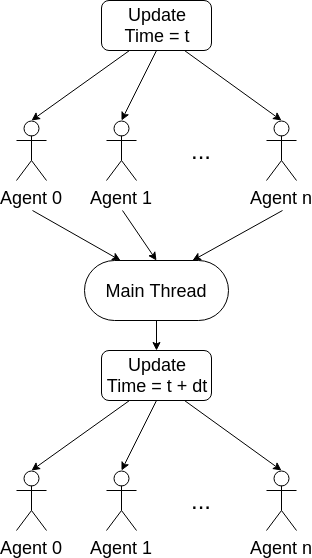
\includegraphics[width=0.4\textwidth, angle=0]{./fig/implabs/parallel.png}
	\caption[Control flow in the parallel update strategy]{Control flow in the parallel update strategy.}
	\label{fig:strategy_par}
\end{figure}

\subsection{Concurrent strategy}
\label{sub:con_strategy}
This strategy has a globally synchronized time-flow but in each time step all the agents are updated in parallel with messages sent and changes to the environment are visible immediately. So this strategy can be understood as a more general form of the \textit{parallel strategy}: all agents run at the same time but act concurrently. It is important to realize that when running agents, which are able to see actions by others immediately, in parallel, we arrive at the very definition of concurrency: parallel execution with mutual read and write access to shared data. Of course this shared data access needs to be synchronized which in turn will introduce event orderings in the execution of the agents. At this point we have a source of inherent non-determinism: although when one ignores any hardware model of concurrency, at some point we need arbitration to decide which agent gets access to a shared resource first, arriving at non-deterministic solutions. This has the very important consequence that repeated runs with the same configuration of the agents and the model may lead to different results. This strategy is of fundamental importance for concurrent ABS in Chapter \ref{ch:concurrent_abs}. See Figure \ref{fig:strategy_conc} for a visualisation of the control flow in this strategy.

\begin{figure}[H]
	\centering
	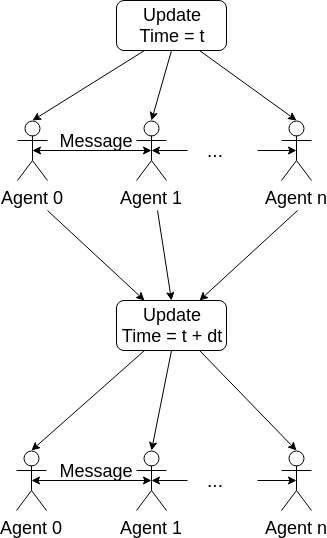
\includegraphics[width=0.5\textwidth, angle=0]{./fig/implabs/concurrent.png}
	\caption[Control flow in the concurrent update strategy]{Control flow in the concurrent update strategy.}
	\label{fig:strategy_conc}
\end{figure}

\subsection{Actor strategy}
\label{sub:act_strategy}
This strategy has no globally synchronized time-flow but all the agents run concurrently in parallel, with their own local time-flow. The messages and changes to the environment are visible as soon as the data arrive at the local agents - this can be immediately when running locally on a multiprocessor or with a significant delay when running in a cluster over a network. Obviously this is also a non-deterministic strategy and repeated runs with the same agent and model configuration may (and will) lead to different results. Information and also time in this strategy is always local to an agent as each agent progresses in its own speed through the simulation. In this case one needs to explicitly \textit{observe} an agent when one wants to extract information from it, for example for visualisation purposes. This observation is then only valid for this current point in time, local to the observer but not to the agent itself, which may have changed immediately after the observation. This implies that we need to sample our agents with observations when wanting to visualize them, which would inherently lead to well known sampling issues. A solution would be to invert the problem and create an observer agent which is known to all agents where each agent sends a \textit{'I have changed'} message with the necessary information to the observer if it has changed its internal state. This also does not guarantee that the observations will really reflect the actual state the agent is in but is a remedy against the notorious sampling. The concept of Actors was proposed by \cite{hewitt_universal_1973} for which \cite{grief_semantics_1975} and \cite{clinger_foundations_1981} developed semantics of different kinds. These works were very influential in the development of the concepts of agents and and can be regarded as foundational basics for ABS. We come back to this strategy in the context of concurrent ABS in Chapter \ref{ch:concurrent_abs}. See Figure \ref{fig:strategy_act} for a visualisation of the control flow in this strategy.

\begin{figure}[H]
	\centering
	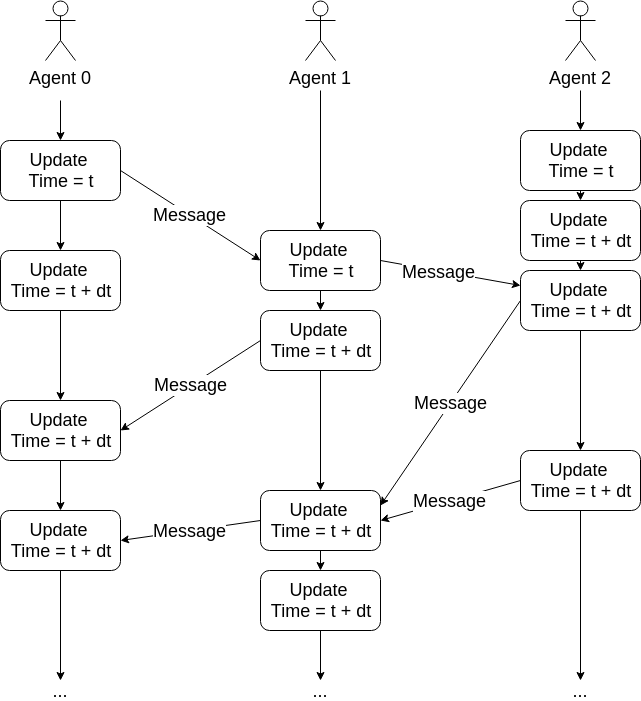
\includegraphics[width=0.5\textwidth, angle=0]{./fig/implabs/actor.png}
	\caption[Control flow in the actor update strategy]{Control flow in the actor update strategy.}
	\label{fig:strategy_act}
\end{figure}

\subsection{Discussion}
In the following chapters we discuss \textit{how} to implement ABS from a pure functional perspective and \textit{why} one would do so. More specifically, we show how to approach the problems discussed in this chapter using pure functional programming. The \textit{sequential} strategy will be covered in depth in Chapter \ref{ch:eventdriven} on event-driven ABS, the \textit{parallel} one in Chapter \ref{ch:timedriven} on time-driven ABS and the \textit{concurrent} strategy is used in Chapter \ref{ch:concurrent_abs} on concurrent ABS. The \textit{actor} strategy is not used in this thesis but its implementation follows directly from the Chapters \ref{ch:timedriven} and \ref{ch:concurrent_abs}: instead of globally synchronising in the main thread, a closed feedback loop is run in every agent thread. 

As already outlined in Chapter \ref{sec:method_abs}, the established approaches implementing ABS use object-oriented programming and thus solve the problems outlined at the start of this chapter from this perspective, which is quite well understood by now, as high quality ABS frameworks like RePast \cite{north_complex_2013} prove. In object-oriented programming an agent is mapped directly onto an object, encapsulating the agents state and providing methods, which implement the agents' actions. Object-orientation allows to expose a well-defined interface using public methods by which one can interact with the agent and query information from it. Agent objects can directly invoke other agents' methods, implicitly mutating the other agents' internal state, which makes direct agent interaction straight forward. Also with object-orientation, agents have global access to an environment for example through a Singleton \cite{gamma_design_1994} or a simple global variable, and can mutate the environments data by direct method calls.

All these language features are not available in functional programming and compared to object-orientation we face seemingly severe restrictions like immutable state, recursion and a static type system. Further, we restrict ourselves deliberately to \textit{pure} functional programming and avoid running in the non-deterministic \texttt{IO} Monad under all costs. The question is then how to solve these problems in functional programming \textit{and} use the restrictions to our advantage. In the next two chapters we show how to implement both a time-driven ABS  using the agent-based SIR model as example (Chapter \ref{ch:timedriven}) and an event-driven ABS using also the SIR and the complex Sugarscape model as examples (Chapter \ref{ch:eventdriven}). In both we present fundamental concepts of how to engineer an ABS from a pure functional programming perspective. This will then be used in subsequent chapters to discuss \textit{why} one would follow a  functional programming approach, identifying its benefits, advantages and also drawbacks over object-oriented approaches. 

%An implementation of an ABS must solve two fundamental problems:
%
%\begin{enumerate}
%	\item \textbf{Source of pro-activity} How can an agent initiate actions without the external stimuli of messages?
%	\item \textbf{Semantics of Messaging} When is a message \textit{m}, sent by agent \textit{A} to agent \textit{B}, visible and processed by \textit{B}?
%\end{enumerate}
%
%In computer systems, pro-activity, the ability to initiate actions on its own without external stimuli, is only possible when there is some internal stimulus, most naturally represented by a continuous increasing time-flow. Due to the discrete nature of computer-system, this time-flow must be discretized in steps as well and each step must be made available to the agent, acting as the internal stimulus. This allows the agent then to perceive time and become proactive depending on time. So we can understand an ABS as a discrete time-simulation where time is broken down into continuous, real-valued or discrete natural-valued time steps. Independent of the representation of the time-flow we have the two fundamental choices whether the time-flow is local to the agent or whether it is a system-global time-flow. Time-flows in computer-systems can only be created through threads of execution where there are two ways of feeding time-flow into an agent. Either it has its own thread-of-execution or the system creates the illusion of its own thread-of-execution by sharing the global thread sequentially among the agents where an agent has to yield the execution back after it has executed its step. Note the similarity to an operating system with cooperative multitasking in the latter case and real multi-processing in the former.
%
%The semantics of messaging define when sent messages are visible to the receivers and when the receivers process them. Message-processing could happen either immediately or delayed, depending on how message-delivery works. There are two ways of message-delivery: immediate or queued. In the case of immediate message-deliver the message is sent directly to the agent without any queuing in between e.g. a direct method-call. This would allow an agent to immediately react to this message as this call of the method transfers the thread-of-execution to the agent. This is not the case in the queued message-delivery where messages are posted to the message-box of an agent and the agent proactively processes the message-box at regular points in time.

% PART II: How
\epigraphhead[450]{}
\part{Towards pure functional ABS}
\section{Time-Driven}
In the following, we derive a pure functional approach for an agent-based SIR model in which we pose solutions to the previously mentioned problems. We start out with a first approach in Yampa and show its limitations. Then we generalise it to a more powerful approach, which utilises Monadic Stream Functions, a generalisation of FRP. Finally we add a structured environment, making the example more interesting and showing the real strength of ABS over other simulation methodologies like System Dynamics and Discrete Event Simulation \footnote{The code of all steps can be accessed freely through the following URL: \url{https://github.com/thalerjonathan/phd/tree/master/public/purefunctionalepidemics/code}}.

\subsection{The SIR model}
The \textit{explanatory} SIR model is a very well studied and understood compartment model from epidemiology \cite{kermack_contribution_1927}, which allows to simulate the dynamics of an infectious disease like influenza, tuberculosis, chicken pox, rubella and measles spreading through a population.

In this model, people in a population of size $N$ can be in either one of three states \textit{Susceptible}, \textit{Infected} or \textit{Recovered} at a particular time, where it is assumed that initially there is at least one infected person in the population. People interact \textit{on average} with a given rate of $\beta$ other people per time-unit and become infected with a given probability $\gamma$ when interacting with an infected person. When infected, a person recovers \textit{on average} after $\delta$ time-units and is then immune to further infections. An interaction between infected persons does not lead to re-infection, thus these interactions are ignored in this model. This definition gives rise to three compartments with the transitions seen in Figure \ref{fig:sir_transitions}.

\begin{figure}
	\centering
	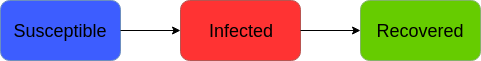
\includegraphics[width=.4\textwidth, angle=0]{./fig/fpabs/timedriven/SIR_transitions.png}
	\caption{States and transitions in the SIR compartment model.}
	\label{fig:sir_transitions}
\end{figure}

This model was also formalized using System Dynamics (SD) \cite{porter_industrial_1962}. In SD one models a system through differential equations, allowing to conveniently express continuous systems, which change over time, solving them by numerically integrating over time, which gives then rise to the dynamics. The SIR model is modelled using the following equation, with the dynamics shown in Figure \ref{fig:sir_sd_dynamics} .

\begin{equation}
\begin{aligned}
\frac{\mathrm d S}{\mathrm d t} = -infectionRate \\
\frac{\mathrm d I}{\mathrm d t} = infectionRate - recoveryRate \\
\frac{\mathrm d R}{\mathrm d t} = recoveryRate 
\end{aligned}
\end{equation}

\begin{equation}
\begin{aligned}
infectionRate = \frac{I \beta S \gamma}{N} \\
recoveryRate = \frac{I}{\delta} 
\end{aligned}
\end{equation}

\begin{figure}
	\centering
	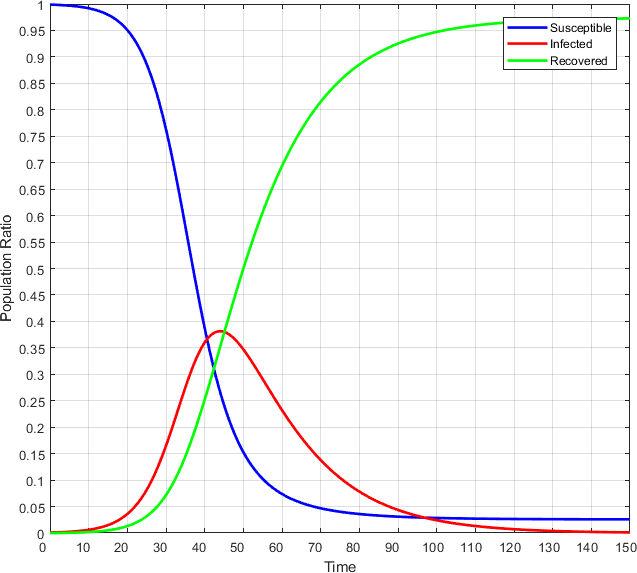
\includegraphics[width=0.5\textwidth, angle=0]{./fig/fpabs/timedriven/SIR_SD_1000agents_150t_001dt.png}
	\caption{Dynamics of the SIR compartment model using the System Dynamics approach. Population Size $N$ = 1,000, contact rate $\beta =  \frac{1}{5}$, infection probability $\gamma = 0.05$, illness duration $\delta = 15$ with initially 1 infected agent. Simulation run for 150 time-steps. Generated using our pure functional SD approach (see Chapter \ref{sub:generalising_system_dynamics}).}
	\label{fig:sir_sd_dynamics}
\end{figure}

The approach of mapping the SIR model to an ABS is to discretize the population and model each person in the population as an individual agent. The transitions between the states are happening due to discrete events caused both by interactions amongst the agents and time-outs. The major advantage of ABS is that it allows to incorporate spatiality as shown in Section \ref{sec:adding_env} and simulate heterogenity of population e.g. different sex, age. This is not possible with other simulation methods e.g. SD or Discrete Event Simulation \cite{zeigler_theory_2000}.

According to the model, every agent makes \textit{on average} contact with $\beta$ random other agents per time unit. In ABS we can only contact discrete agents thus we model this by generating a random event on average every $\frac{1}{\beta}$ time units. We need to sample from an exponential distribution because the rate is proportional to the size of the population \cite{borshchev_system_2004}. Note that an agent does not know the other agents' state when making contact with it, thus we need a mechanism in which agents reveal their state in which they are in \textit{at the moment of making contact}. This mechanism is an implementation detail, which we will derive in our implementation steps. For now we only assume that agents can make contact with each other somehow.

The \textit{parallel} strategy matches the semantics of the agent-based SIR model due to the underlying roots in the System Dynamics approach. As discussed already in Chapter \ref{sub:par_strategy}, in the parallel update-strategy, the agents act conceptually all at the same time in lock-step. This implies that they observe the same environment state during a time-step and actions of an agent
are only visible in the next time-step - they are isolated from each other. As will become apparent, FP can be used to enforce the correct application of this strategy already on the compile-time level.

\subsection{A pure functional implementation}
TODO: follow the PFE paper but add a few references back to the implementing ABS chapter so it is clear what problems we are currently solving. also might explain some concepts bit more in depth e.g. continuations?

As described in the Chapter \ref{sec:back_frp}, Arrowized FRP \cite{hughes_generalising_2000} is a way to implement systems  with continuous and discrete time-semantics where the central concept is the signal function, which can be understood as a process over time, mapping an input- to an output-signal. Technically speaking, a signal function is a continuation which allows to capture state using closures and hides away the $\Delta t$, which means that it is never exposed explicitly to the programmer, meaning it cannot be manipulated.

As already pointed out, agents need to perceive time, which means that the concept of processes over time is an ideal match for our agents and our system as a whole, thus we will implement them and the whole system as signal functions.

\subsection{Discussion}
Our FRP based approach is different from traditional approaches in the ABS community. First it builds on the already quite powerful FRP paradigm. Second, due to our continuous time approach, it forces one to think properly of time-semantics of the model and how small $\Delta t$ should be. Third it requires one to think about agent interactions in a new way instead of being just method-calls.

Because no part of the simulation runs in the IO Monad and we do not use \textit{unsafePerformIO} we can rule out a serious class of bugs caused by implicit data-dependencies and side-effects, which can occur in traditional imperative implementations.

Also we can statically guarantee the reproducibility of the simulation, which means that repeated runs with the same initial conditions are guaranteed to result in the same dynamics. Although we allow side-effects within agents, we restrict them to only the Random Monad in a controlled, deterministic way and never use the IO Monad, which guarantees the absence of non-deterministic side effects within the agents and other parts of the simulation.

Determinism is also ensured by fixing the $\Delta t$ and not making it dependent on the performance of e.g. a rendering-loop or other system-dependent sources of non-determinism as described by \cite{perez_testing_2017}. Also by using FRP we gain all the benefits from it and can use research on testing, debugging and exploring FRP systems \cite{perez_testing_2017, perez_back_2017}.

Also we showed how to implement the \textit{parallel} update-strategy \cite{thaler_art_2017} in a way that the correct semantics are enforced and guaranteed already at compile time through the types. This is not possible in traditional imperative implementations and poses another unique benefit over the use of functional programming in ABS.

The result of using FRP allows expressing continuous time-semantics in a very clear, compositional and declarative way, abstracting away the low-level details of time-stepping and progress of time within an agent.
	
Our approach can guarantee reproducibility already at compile time, which means that repeated runs of the simulation with the same initial conditions will always result in the same dynamics, something highly desirable in simulation in general. This can only be achieved through purity, which guarantees the absence of implicit side-effects, which allows to rule out non-deterministic influences at compile time through the strong static type system, something not possible with traditional object-oriented approaches. Further, through purity and the strong static type system, we can rule out important classes of run-time bugs e.g. related to dynamic typing, and the lack of implicit data-dependencies which are common in traditional imperative object-oriented approaches.
	
Using pure functional programming, we can enforce the correct semantics of agent execution through types where we demonstrate that this allows us to have both, sequential monadic behaviour, and agents acting \textit{conceptually} at the same time in lock-step, something not possible using traditional object-oriented approaches.

Currently, the performance of the system does not come close to imperative implementations. We compared the performance of our pure functional approach as presented in Section \ref{sec:adding_env} to an implementation in Java using the ABS library RePast \cite{north_complex_2013}. We ran the simulation until $t = 100$ on a 51x51 (2,601 agents) with $\Delta t = 0.1$ (unknown in RePast) and averaged 8 runs. The performance results make the lack of speed of our approach quite clear: the pure functional approach needs around 72.5 seconds whereas the Java RePast version just 10.8 seconds on our machine to arrive at $t = 100$. It must be mentioned, that RePast does implement an event-driven approach to ABS, which can be much more performant \cite{meyer_event-driven_2014} than a time-driven one as ours, so the comparison is not completely valid. Still, we have already started investigating speeding up performance through the use of Software Transactional Memory \cite{harris_composable_2005, harris_transactional_2006}, which is quite straight forward when using MSFs. It shows very good results but we have to leave the investigation and optimization of the performance aspect of our approach for further research as it is beyond the scope of this paper.

Despite the strengths and benefits we get by leveraging on FRP, there are errors that are not raised at compile time, e.g. we can still have infinite loops and run-time errors. This was for example investigated in \cite{sculthorpe_safe_2009} where the authors use dependent types to avoid some run-time errors in FRP. We suggest that one could go further and develop a domain specific type system for FRP that makes the FRP based ABS more predictable and that would support further mathematical analysis of its properties. Furthermore, moving to dependent types would pose a unique benefit over the traditional object-oriented approach and should allow us to express and guarantee even more properties at compile time. We leave this for further research.

In our pure functional approach, agent identity is not as clear as in traditional object-oriented programming, where there is a quite clear concept of object-identity through the encapsulation of data and methods. Signal functions don't offer this strong identity and one needs to build additional identity mechanisms on top e.g. when sending messages to specific agents.

We can conclude that the main difficulty of a pure functional approach evolves around the communication and interaction between agents, which is a direct consequence of the issue with agent identity. Agent interaction is straight-forward in object-oriented programming, where it is achieved using method-calls mutating the internal state of the agent, but that comes at the cost of a new class of bugs due to implicit data flow. In pure functional programming these data flows are explicit but our current approach of feeding back the states of all agents as inputs is not very general. We have added further mechanisms of agent interaction which we had to omit due to lack of space.

\subsection{Other approaches}
Sequential: see event-driven
Concurrent: see STM chapter
Actor: not discussed in this thesis but briefly 

\subsection{Super-Sampling}
when super-sampling is mentioned in the PFE paper extend it and add FrABS report, also show superSampling function implementation from PFE paper and FrABS with full body implementation

\chapter{Pure functional event-driven ABS}
\label{ch:eventdriven}

In this chapter we build on the previous discussion of update strategies in Chapter \ref{ch:impl_abs} and the implementation techniques presented in the time-driven approach of Chapter \ref{ch:timedriven} to develop concepts for event-driven ABS in a pure functional way. 

\medskip

In event-driven ABS \cite{meyer_event-driven_2014}, the simulation is advanced through events: agents and the environment schedule events into the future and react to incoming events scheduled by themselves, other agents, the environment or the simulation kernel. Time is discrete in this approach: it advances step-wise from event to event, where each event has an associated receiver and $\Delta t$, indicating the delay to the current virtual simulation time when should be scheduled. This implies that time could stay constant, for example when an event is scheduled with $\Delta t = 0$ the virtual simulation time does not advance. Further, agents can schedule events to themselves, emulating a recurring behaviour, which in turn emulates pro-active behaviour. Because agents can adopt and change their state and behaviour when processing an event, this means that even if time does not advance, agents can change. This non-signal behaviour is the fundamental difference to the time-driven approach in Chapter \ref{ch:timedriven}. Further, this mechanism is used to implement synchronous agent interactions pure functionally as discussed in the respective sections below.

The event-driven approach makes the simulation kernel technically closely related to a Discrete Event Simulation (DES) \cite{zeigler_theory_2000}. Due to the necessity of imposing a correct ordering of events in this type of ABS, it needs to be stepped event by event, with the \textit{sequential} update strategy, as introduced in Chapter \ref{sec:seq_strategy}. It is important to emphasise that only the semantics of the sequential update strategy allow the kind of features  presented in the following sections, as the agents act one after the other, seeing the effects of previous agents in the same time step. This would not make sense in the parallel update strategy as used in time-driven ABS, where agents act conceptually at the same time - event-driven ABS is inherently sequential due to its fundamental reliance on effects as will become clearer in the sections below. Note that there exists also Parallel DES (PDES) \cite{fujimoto_parallel_1990}, which processes events in parallel and deals with inconsistencies by reverting to consistent states. We hypothesise that a pure functional approach could be beneficial in such an approach due to persistent data structures and explicit handling of side effects but we leave this for further research.

\medskip

We start introducing the concepts of agent identity and event scheduling utilising both \textit{Reader} and \textit{Writer} Monads. We do this by using an event-driven agent-based SIR model, inspired by \cite{macal_agent-based_2010}. We then use the highly complex Sugarscape model as introduced in Chapter \ref{sec:sugarscape}, to develop more advanced features of ABS in a pure functional context: dynamic creation and removal of agents during simulation, adding a shared mutable environment, local mutable agent state and synchronous agent interactions. 
%Note that the Sugarscape model is not a real event-driven model like the event-driven SIR one is as in it the agents do schedule events but they don't do this into the future - events in Sugarscape don't have associated time-stamps.

\section{Basics of event-driven ABS}
\label{sec:eventdriven_basics}

In this section we derive the basics of event-driven ABS using the SIR model, as introduced in Chapter \ref{sec:sir_model}, with an event-driven approach inspired by \cite{macal_agent-based_2010}. Although it is a fundamentally different approach to ABS than the time-driven implementation in Chapter \ref{sec:timedriven_firststep} both solutions are quantitatively equal as they produce the same class of dynamics. Qualitatively they fundamentally differ though in terms of expressivity and performance as we will see in the discussion.

The basics of event-driven ABS are the concept of agent identity, events and event-scheduling. We introduce them step-by-step using various Monads and then generalise to a \textit{tagless final} approach, which has various benefits as pointed out in the respective section. 

\subsection{An event-driven SIR}
Before we can derive implementation concepts, we first need to discuss how an event-driven SIR model works, as inspired by \cite{macal_agent-based_2010}. Fundamentally, what is required is to transform all time-dependent behaviour and agent interactions into the scheduling and receiving of events. For the SIR this should be trivial and straightforward, taking inspiration from the time-driven implementation, where we simply translate the occurrences of events generated by \textit{occasionally} into scheduling of events. For agent interactions we also use events, making this more explicit than in the time-driven approach. As already pointed out, assuming that events have a receiver and a scheduling time given as $\Delta t$ relative to the current simulation time, we end up with three event-types:

\begin{enumerate}
	\item \textbf{MakeContact} - is used to let susceptible agents pro-actively make contact with $\beta$ (contact rate) other agents per 1 time-unit.
	\item \textbf{Contact$_{Sender, \ SIRState}$} - is used to make contact between agents where, agents reveal their state by sending or replying their current state.
	\item \textbf{Recover} - is used to let infected agents recover pro-actively after the given $\delta$ (illness duration). 
\end{enumerate}

Now we can give a concise definition of all three agent behaviours:

\paragraph{Susceptible Agent}
\begin{itemize}
	\item A susceptible agent initially schedules a \textit{MakeContact} event with $\Delta t = 1$ to itself.
	\item When receiving \textit{MakeContact}, the agent sends a \textit{Contact} event to $\beta$ (contact rate) random other agents with $\Delta t = 0$ and \textit{SIRState} of \textit{Susceptible}, resulting in these events to be scheduled immediately. Further, the agent schedules \textit{MakeContact} with $\Delta t = 1$ to itself, to keep the pro-active process of making contact with other agents active.
	\item When the agent receives a \textit{Contact} event, it checks if it is from an infected agent (\textit{SIRState} is \textit{Infected}). If the event is not from an infected agent, it ignores it, otherwise it becomes infected with a given probability.
\end{itemize}

\paragraph{Infected Agent}
\begin{itemize}
	\item An infected agent initially schedules a \textit{Recover} event to itself, with an exponentially distributed random $\Delta t$ of $\delta$ (illness duration).
	\item When the agent receives a \textit{Contact} event, it checks if it is from a susceptible agent (\textit{SIRState} is \textit{Susceptible}). If the event is not from a susceptible agent, it ignores it, otherwise it simply replies to this susceptible agent with a \textit{Contact} event with $\Delta t = 0$ and and \textit{SIRState} of \textit{Infected}.
\end{itemize}

\paragraph{Recovered Agent}
The recovered agent does not change any more, reacts to no incoming events and schedules no events - it stays constantly \textit{Recovered} forever.

\medskip

It is easy to see that this behaviour emulates the time-driven one and indeed in Figure \ref{fig:sir_eventdriven_dynamics} it is also visually clear that it produces similar dynamics. A striking difference are the small spikes and steps in the dynamics, which stem from the fact that time advances discretely and not continuous as in the time-driven implementation. In Chapter \ref{ch:sir_invariants}, we use property-based testing to show that both implementations indeed produce similar distributions in their dynamics, thus putting the claim that both implementations are quantitatively equal on a much more robust ground.

\begin{figure}
	\centering
	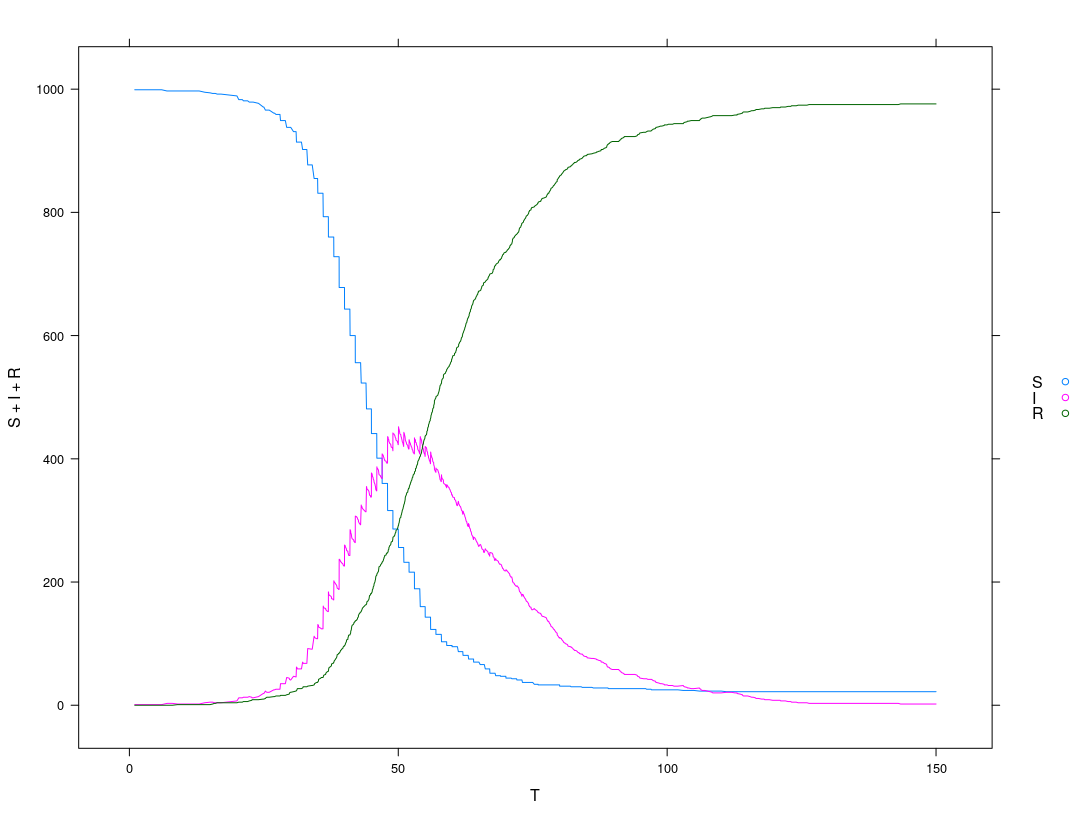
\includegraphics[width=0.7\textwidth, angle=0]{./fig/eventdriven/sir_eventdriven.png}
	\caption{Dynamics of the event-driven SIR model. Population Size $N$ = 1,000, contact rate $\beta = \frac{1}{5}$, infection probability $\gamma = 0.05$, illness duration $\delta = 15$ with initially 1 infected agent. Simulation run for 150 time-steps.}
	\label{fig:sir_eventdriven_dynamics}
\end{figure}

\subsection{Events, Agent Identity and Scheduling}
We can now start to discuss the concepts from an implementation perspective. First, we need to make the concept of an event explicit: they are of a given type, have a receiver and a time-stamp in \textit{absolute} simulation time when they shall be scheduled. We keep the event-type polymorphic and represent the receiver by an \textit{AgentId} which is a simple \textit{Int}. For efficient scheduling, the events are kept in a priority-queue \footnote{We are using the \textit{Data.PQueue.Min} implementation from the \textit{pqueue} package.}, sorted ascending by the time-stamp. Thus we define the following:

\begin{HaskellCode}
type Time        = Double
type AgentId     = Int
data QueueItem e = QueueItem e AgentId Time

-- the event priority-queue
type EventQueue e = PQ.MinQueue (QueueItem e)

-- implement Ord for QueueItem for acended sorting
instance Ord (QueueItem e) where
  compare (QueueItem _ _ t1) (QueueItem _ _ t2) = compare t1 t2
\end{HaskellCode}

Next, we define a polymorphic type for the agent. In event-driven ABS, due to the fact that agents are not signals any more, we abandon time-aware signal functions of BearRiver from the previous chapter and focus solely on Monadic Stream Functions (MSF). In event-driven ABS agents receive events, thus as input to an \textit{MSF} the polymorphic event type \textit{e} is used. As output, the polymorphic output type \textit{o} is used, which will be instantiated to a specific monomorphic type in the SIR model below. The question is now what Monad shall be used. For scheduling purposes (and because models might require it), agents should be able to \textit{read} the current simulation time: this is accomplished through a \textit{ReaderT Time}. Further, agents should be able to \textit{read} the identities of the other agents available in the simulation so they can schedule events to them when necessary: this is accomplished through a \textit{ReaderT [AgentId]}. Most importantly, agents have to be able to schedule events, meaning they have to be able to \textit{write} the events into some sink where they are accumulated for scheduling: this is accomplished through a \textit{WriterT [QueueItem e]}. Finally, the transformer stack needs to be extendible by other Monads, specified in concrete models like the SIR below, so we add another polymorphic type \textit{m}, indicating the closing Monad (stack).

\begin{HaskellCode}
type ABSMonad m e   = ReaderT Time (WriterT [QueueItem e] (ReaderT [AgentId] m))
type AgentMSF m e o = MSF (ABSMonad m e) e o
\end{HaskellCode}

Note that BearRivers \textit{SF} has also a \textit{ReaderT Double} as the innermost Monad but we deliberately avoided its use because the intended semantics of an \textit{SF} are different: the value in the \textit{ReaderT} of the \textit{SF} represents the sampling time-delta and not the absolute time, as in the event-driven case.

We can already implement a few polymorphic functions, operating on the given Monad stack. First, we implement a function \textit{allAgentIds} which simply returns the \textit{AgentId} of all agents, the contents of the \textit{ReaderT [AgentId]}. Second, we implement a function \textit{scheduleEvent} which allows to schedule a given event to a given receiver into the future given a specific time-delay, relative to the current simulation time.
 
\begin{HaskellCode}
allAgentIds :: Monad m => (ABSMonad m e) [AgentId]
allAgentIds = lift (lift ask)

scheduleEvent :: Monad m
              => e        -- ^ event
              -> AgentId  -- ^ receiver
              -> Double   -- ^ time-delay
              -> (ABSMonad m e) ()
scheduleEvent e aid dt = do
  -- get current simulation time
  t <- ask
  -- construct queue item
  let q = QueueItem e aid (t + dt)
  -- write/append (tell) to the WriterT (QueueItem e)
  lift (tell [q])
\end{HaskellCode}

Processing events can also be implemented generically and is straight forward, thus we only discuss the subtleties. For efficient lookup of event receivers all agents are organised into an \textit{IntMap}, which also holds the current output of the agent, to allow sampling of the domain-state. In general, the domain-state is highly model specific, thus a generic implementation needs to offer some mechanism to update the domain-state after an event, a process we named domain-state sampling. Our approach is to call a function which receives the agent map and returns a new domain-state for the current event/time-step. These domain-states are appended to an infinite list which forms the output of the simulation.

The events are then processed in the order provided by the queue and each event is executed with the given receiver. Running a receiver is simply achieved using the agent map, where a reviver is looked up and its \textit{MSF} is evaluated with the given event as input and the resulting monadic actions executed with the given information.
 
\subsection{Parametrising for SIR}
With the generic concepts now established, we show how to parametrise them to the concrete SIR model. First, we define the already well known states the agents can be in and the three different event types, as already introduced above.

\begin{HaskellCode}
data SIRState = Susceptible | Infected | Recovered
data SIREvent = MakeContact | Contact AgentId SIRState | Recover 
\end{HaskellCode}

Next, we parametrise the \textit{ABSMonad} to the SIR model: because behaviour is stochastic, we need to make use of the \textit{Rand} Monad, which also closes the Monad stack of \textit{ABSMonad}. Further, the event type is obviously parametrised to \textit{SIREvent}.

\begin{HaskellCode}
type SIRMonad g = ABSMonad (Rand g) SIREvent
\end{HaskellCode}

Now we define a \textit{SIRAgent} which can be understood as a constructing function, run once upon construction of the agent. This constructing functions runs in the \textit{SIRMonad}, thus agents can already make full use of the functionality, so they can schedule initial events, depending on their initial state. This is important for the susceptible and infected agent, which both need to schedule initial events for pro-active behaviour. The constructing functions also takes the \textit{AgentId} of the agent, thus making it available to the agent at construction time. It returns the initial agent-behaviour as \textit{AgentMSF}.

\begin{HaskellCode}
type SIRAgent g 
       = AgentId -> (SIRMonad g) (AgentMSF (SIRMonad g) SIREvent SIRState)
\end{HaskellCode}

The implementation of the constructing function of type \textit{SIRAgent} is straight forward and follows the specification given above. It makes use of the functions \textit{scheduleMakeContact} and \textit{scheduleRecovery} which are implemented using the generic \textit{scheduleEvent} from above.

\begin{HaskellCode}
sirAgent :: RandomGen g 
         => Int         -- ^ contact rate (beta)
         -> Double      -- ^ infectivity (gamma)
         -> Double      -- ^ illness duration (delta)
         -> SIRState    -- ^ initial state of the agent
         -> SIRAgent g
sirAgent beta gamma delta Susceptible aid = do
  -- on start, schedule MakeContact to itself
  scheduleMakeContact aid 1
  -- return susceptible behaviour
  return (susceptibleAgent aid beta gamma delta)
sirAgent _ _ delta Infected aid = do
  -- on start, schedule Recover to itself
  scheduleRecovery aid delta
  -- return infected behaviour
  return (infectedAgent aid)
sirAgent _ _ _ Recovered _ = 
  -- simply return recovered behaviour
  return recoveredAgent

scheduleMakeContact :: RandomGen g => AgentId -> Double -> (SIRMonadT g) ()
scheduleMakeContact aid = scheduleEvent MakeContact aid

scheduleRecovery :: RandomGen g => AgentId -> Double -> (SIRMonadT g) ()
scheduleRecovery aid delta = do
  dt <- (lift . lift . lift) (randomExpM (1 / delta))
  scheduleEvent Recover aid dt

-- returns random value following exponential distribution with given lambda
randomExpM :: MonadRandom m => Double -> m Double
\end{HaskellCode}

Now we are finally ready to implement the actual behaviour of an agent, where we discuss the full implementation of the susceptible agent behaviour. The basic structure should be already familiar from the time-driven approach, using \textit{switch} to dynamically change the behaviour to \textit{infectedAgent} in case of an infection. The behaviour is then a simple event handler, pattern matching on the incoming events:

\begin{HaskellCode}
susceptibleAgent :: RandomGen g 
                 => AgentId        -- ^ agents id
                 -> Int            -- ^ contact rate (beta)
                 -> Double         -- ^ infectivity (gamma)
                 -> Double         -- ^ illness duration (delta)
                 -> SIRAgentMSF g
susceptibleAgent aid beta gamma delta = 
    switch susceptibleAgentInfected (const (infectedAgent aid))
  where
    susceptibleAgentInfected :: RandomGen g 
                             => MSF (SIRMonadT g) SIREvent (SIRState, Maybe ()) 
    susceptibleAgentInfected = proc e -> do
      -- handle incoming event in monadic action
      ret <- arrM handleEvent -< e
      case ret of
        Nothing -> returnA -< (Susceptible, ret)
        _       -> returnA -< (Infected, ret)
\end{HaskellCode}

We strictly follow the specification as above. In case the agent receives \textit{Contact} from an infected agent it might become infected with a given probability. If it becomes infected, it schedules the recovery as it will make the transition to an infected agent.

\begin{HaskellCode}
-- received Contact from an Infected agent
handleEvent :: RandomGen g => SIREvent -> (SIRMonadT g) (Maybe ())
handleEvent (Contact _ Infected) = do
  -- become infected with gamma probability
  r <- (lift . lift . lift) (randomBoolM gamma)
  if r
    -- got infected 
    then do
      -- schedule Recovery to self, because switching to infected
      scheduleRecovery aid delta
      return (Just ())
    -- no infection
    else return Nothing

-- returns True with given probability
randomBoolM :: MonadRandom m => Double -> m Bool
\end{HaskellCode}

In case the agent receivers \textit{MakeContact} from itself, it will send \textit{Contact} with \textit{Susceptible} to $\beta$ (contact rate) other agents without delay and \textit{MakeContact} to itself with a delay of 1 time unit.

\begin{HaskellCode}
-- received MakeContact (from itself)
handleEvent MakeContact = do
  ais <- allAgentIds
  -- get beta random agents
  receivers <- (lift . lift . lift) (forM [1..beta] (const (randomElemM ais)))
  -- make contact with random agents
  mapM_ makeContactWith receivers
  -- re-schedule MakeContact to self
  scheduleMakeContact aid 1
  return Nothing
  
makeContactWith :: AgentId -> (SIRMonadT g) ()
makeContactWith receiver = 
  -- schedule Contact event immediately
  scheduleEvent (Contact aid Susceptible) receiver 0

-- picks an element randomly from the (non empty) list
randomElemM :: MonadRandom m => [e] -> m e
\end{HaskellCode}

The infected and recovered behaviours are conceptually equivalent and thus left as a trivial exercise to the reader. 

\subsection{Tagless Final}
At this point, the basics of event-driven ABS should be clear: how events are represented and processed using an event queue, how agents are represented with an \textit{MSF} and the idea behind the underlying polymorphic Monad transformer stack. Further, by parametrising the polymorphic concepts to the SIR model, we showed how to instantiate the generic concepts into a concrete model to arrive at a robust, maintainable and solid solution which is very likely to be correct up to the initial informal specification.

\medskip

In this section we briefly want to show how the so-called \textit{tagless final} approach \cite{kiselyov_typed_2012} can be used to arrive at a cleaner and more extensible interface of our implementation, which is also open to different \textit{interpretations}. The idea behind \textit{tagless final} is simple: specify the interface of operations in a typeclass and then write one or multiple interpreters for it, which simply means writing an instance implementation for the given typeclass. We start by defining the typeclass \textit{MonadAgent} with all the necessary methods, making up the effectful API of our agents. Note that we need to enable two language extensions: \textit{MultiParamTypeClasses} because we want to have more than a single type parameter in the typeclass - besides the Monad \textit{m}, we also want to parametrise over the event type \textit{e}; \textit{FunctionalDependencies} because the event type \textit{e} is determined by the Monad type \textit{m}.

\begin{HaskellCode}
{-# LANGUAGE MultiParamTypeClasses  #-}
{-# LANGUAGE FunctionalDependencies #-}

class Monad m => MonadAgent e m | m -> e where
  randomBool  :: Double -> m Bool
  randomExp   :: Double -> m Double
  randomElem  :: [a] -> m a
  getAgentIds :: m [AgentId]
  getTime     :: m Time
  getMyId     :: m AgentId
  schedEvent  :: e -> AgentId -> Double -> m ()
\end{HaskellCode}

The methods are self explaining. This typeclass is now used to replace the Monad stack by an overloaded type definition in the respective functions. Thus, the implementation of the agent constructing function and the agent behaviours are the same, with only the types changing slightly, lifts becoming obsolete and calls to function replaced by calls to methods of the typeclass. We don't give the full implementation again but only the type of the agent construction function as example, the types of the agent behaviours follow a similar pattern: 

\begin{HaskellCode}
sirAgent :: MonadAgent SIREvent m  -- CHANGED: overloaded with typeclass
         => Int         -- ^ contact rate (beta)
         -> Double      -- ^ infectivity (gamma)
         -> Double      -- ^ illness duration (delta)
         -> SIRState    -- ^ initial state of the agent
         -> m (MSF m SIREvent SIRState) -- CHANGED: no Monad stack
\end{HaskellCode}

Note that we added a \textit{getMyId} method, which shall return the \textit{AgentId} of the agent itself, avoiding the need for the agent of keeping the agent id around and also making it possible to implement more robust self-scheduling functions. For example, the \textit{scheduleRecovery} function is implemented in the \textit{tagless final} approach in the following way:

\begin{HaskellCode}
scheduleRecovery :: MonadAgent SIREvent m => Double -> m ()
scheduleRecovery delta = do
  -- draw random value from exponential distribution
  dt <- randomExp (1 / delta)
  -- get id of agent, no more need to pass it explicitly
  ai <- getMyId
  -- schedule Recover to itself
  schedEvent Recover ai dt
\end{HaskellCode}

What we are missing is a \textit{pure} interpreter for the agent implementation and the \textit{MonadAgent} typeclass. We start by defining a \textit{newtype}, which basically is a conceptually similar Monad stack as in the original implementation without the \textit{tagless final} approach. We let Haskell automatically derive monadic typeclasses, Functor, Applicative and Monad instances which saves a lot of boiler plate code, for which the \textit{GeneralizedNewtypeDeriving} language extension is required. Instead of the \textit{Rand} Monad, a \textit{StateT SimState} is used, which carries the random-number generator and other data  for synchronous agent interactions as will be discussed in the respective sections.

\begin{HaskellCode}
{-# LANGUAGE GeneralizedNewtypeDeriving #-}

newtype SIRAgentPure a = SIRAgentPure 
  { unSirAgentPure :: ReaderT (Time, AgentId, [AgentId]) -- combined into one
                        (WriterT [QueueItem SIREvent]
                          (State SimState)) a}
  deriving (Functor, Applicative, Monad, 
            MonadReader (Time, AgentId, [AgentId]),
            MonadWriter [QueueItem SIREvent],  
            MonadState SimState)
\end{HaskellCode}

Having this \textit{newtype} we can now write a \textit{pure} interpreter for the \textit{MonadAgent}. The implementations are straight forward and should be self explanatory. To run \textit{Rand} Monad actions, the function \textit{runRandWithSimState} is used, which extracts the random-number generator from \textit{SimState}, runs the action and puts the changed random-number generator back into the \textit{SimState}.

\begin{HaskellCode}   
{-# LANGUAGE FlexibleContexts           #-}
{-# LANGUAGE MultiParamTypeClasses      #-}
      
instance MonadAgent SIREvent SIRAgentPure where
  randomBool = runRandWithSimState . randomBoolM
  randomElem = runRandWithSimState . randomElemM
  randomExp  = runRandWithSimState . randomExpM
  -- schedEvent :: SIREvent -> AgentId -> Double -> m ()
  schedEvent e receiver dt = do
    t <- getTime 
    tell [QueueItem e receiver (t + dt)]
  -- getAgentIds :: m [AgentId]
  getAgentIds = asks trd
  -- getTime :: m Time
  getTime = asks fst3
  -- getMyId :: m AgentId
  getMyId = asks snd3

fst3 :: (a,b,c) -> a
snd3 :: (a,b,c) -> b
trd :: (a,b,c) -> c
runRandWithSimState :: MonadState SimState m => Rand StdGen a -> m a
\end{HaskellCode}

The main benefit of a \textit{tagless final} approach is that it is a solution to the expression problem \cite{kiselyov_typed_2012}: it is possible to add new interpreters of an embedded language and add new functionality without breaking the existing implementations. Interpretation in our case means that we can use different underlying Monads to run the agents: if we want to guarantee purity, no \textit{IO} Monad shall be used. Otherwise when concurrency with a lock-based approach or a lock-free approach is required \textit{IO} or \textit{STM} can be used in the underlying interpreter. Also, for reproducible unit testing, one can write custom test-interpreters where methods always return a-priori known results, similar to mocking. Adding new functionality is less an issue here but might become highly important when designing a more general ABS library, building on the \textit{tagless final} approach. It would allow the user of such a library to extend existing agents or default behaviour with new, custom-built methods, without breaking the existing ones. We leave that for further research.

\section{Advanced features}
\label{sec:advanced_eventdriven_ABS}

In the previous section we established the basics of event-driven ABS. It is now clear how events are represented, how agent identity is handled, how agents receive and schedule events, how events are scheduled and domain state is sampled. Furthermore, by using the \textit{tagless final} approach, we arrived at an elegant, extensible and robust solution, which separates specification, the agent and its behaviour, from its implementation, a \textit{pure} interpreter. 

In this section we present more advanced concepts of event-driven ABS, necessary in models with much higher complexity than the simple SIR. We developed these concepts using the Sugarscape model as introduced in Chapter \ref{sec:sugarscape}. Consequently we will discuss them from this model's perspective. More specifically, we show how to create and remove agents dynamically during simulation, add a shared mutable environment, model local mutable agent state and finally how synchronous agent interactions can be implemented. Together with the basics of event-driven ABS, with these concepts established it should be possible to implement a wide range of event-driven ABS models. For this we developed a full implementation of the Sugarscape model, in which we explored the concepts presented in this chapter, with the code accessible from the \href{https://github.com/thalerjonathan/haskell-sugarscape}{code repository}~\cite{thaler_sugarscape_repository}.

\section{Case Study II: Sugarscape}
\label{sec:sugarscape_concurrent}
The second case study is the Sugarscape model as introduced in Chapter \ref{sec:sugarscape}. In this case study we look into the potential performance improvement in a model with much more complex agent behaviour and dramatically increased writes on the shared environment.

We implemented the \textit{Carrying Capacity} (p. 30) section of Chapter II of the Sugarscape book \cite{epstein_growing_1996}. In each step agents search (move) to the cell with the most sugar they see within their vision, harvest all of it from the environment and consume sugar because of their metabolism. Sugar regrows in the environment over time. Only one agent can occupy a cell at a time. Agents don't age and cannot die from age. If agents run out of sugar due to their metabolism, they die from starvation and are removed from the simulation. The authors report that the initial number of agents quickly drops and stabilises around a level depending on the model parameters. This is in accordance with our results as we show in Chapter \ref{ch:property} and guarantees that we don't run out of agents. The model parameters are as follows:

\begin{itemize}
	\item Sugar Endowment: each agent has an initial sugar endowment randomly uniform distributed between 5 and 25 units;
	\item Sugar Metabolism: each agent has a sugar metabolism randomly uniform distributed between 1 and 5;
	\item Agent Vision: each agent has a vision randomly uniform distributed between 1 and 6, same for each of the 4 directions (N, W, S, E);
	\item Sugar Growback: sugar grows back by 1.0 unit per step until the maximum capacity of a cell is reached;
	\item Agent Number: initially 500 agents;
	\item Environment Size: 50 x 50 cells with toroid boundaries which wrap around in both x and y dimension.
\end{itemize}

Note that in this implementation (as in the full Chapter II of the book), no direct and no synchronous agent-interactions as we implemented them in Chapter \ref{sec:eventdriven_implementation} are happening. As in the SIR example, all agents interact with each other indirectly through the shared environment. This allows us to regard the implementation as a time-driven, parallel one wherein each step agents act conceptually at the same time.

We compare four different implementations \footnote{The code is freely available at \url{https://github.com/thalerjonathan/phd/tree/master/public/stmabs/code/SugarScape}}:

\begin{enumerate}
	\item Sequential - All agents are run after another (including the environment) and the environment is shared amongst the agents using a \textit{StateT} transformer.
	\item Lock-Based - All agents are run concurrently in the \textit{IO} monad and the environment is shared between the agents, using an \textit{IORef} with the access synchronised through an \textit{MVar} lock.
	\item STM TVar - All agents are run concurrently in the \textit{STM} monad and the environment is shared using a \textit{TVar} between the agents.
	\item STM TArray - All agents are run concurrently in the \textit{STM} monad and the environment is shared using a \textit{TArray} between the agents. 
\end{enumerate}

We follow \cite{lysenko_framework_2008} and measure the average number of steps per second of the simulation over 60 seconds. For each experiment we conducted 8 runs on our machine (see Table \ref{tab:machine_specs}) under no additional work-load and report the average. In the experiments we varied the number of cores when running concurrently - the numbers are always indicated clearly.

%\paragraph{Output} Note that we omit the graphical rendering in the functional approach because it is a serious bottleneck taking up substantial amount of the simulation time. Although visual output is often important in ABS, it is not what we are interested here thus we completely omit it and only output the number of agents in the simulation at each step piped into a file, thus omitting slow output to the console \footnote{Note that we need to produce \textit{some} output because of Haskells laziness - if we wouldn't output anything from the simulation then the expressions would actually never be fully evaluated thus resulting in high number of steps per second but which obviously don't really reflect the true computations done.}.

\paragraph{Ordering} The model specification requires to shuffle agents before every step (Footnote 12 on page 26 \cite{epstein_growing_1996}). In the \textit{Sequential} approach we do this explicitly but in the \textit{Lock-Based} and both \textit{STM} approaches we assume this to happen automatically due to race-conditions in concurrency, thus we arrive at an effectively shuffled processing of agents: we implicitly assume that the order of the agents is \textit{effectively} random in every step. The important difference between the two approaches is that in the \textit{Sequential} approach we have full control over this randomness but in the \textit{STM} not - also this means that repeated runs with the same initial conditions might lead to slightly different results. 
This decision leaves the execution order of the agents ultimately to Haskell's Runtime System and the underlying OS. We are aware that by doing this, we make assumptions that the threads run uniformly distributed (fair) but such assumptions should not be made in concurrent programming. As a result we can expect this fact to produces non-uniform distributions of agent runs but we assumed that for this model this does not has a significance influence - in case of doubt, we could resort to shuffling the agents before running them in every step. We agree that this very problem would deserve in-depth research on its own, where also the influence of non-deterministic ordering on the correctness and results of ABS has to be analysed. This is not the main interest of this section though and we leave it for further research as it is completely beyond the focus of this thesis.

%Note that in the concurrent implementations we have two options for running the environment: either asynchronously as a concurrent agent at the same time with the population agents or synchronously after all agents have run. We must be careful though as running the environment as a concurrent agent can be seen as conceptually wrong because the time when the regrowth of the sugar happens is now completely random. In this case it could happen that sugar regrows in the very first transaction or in the very last, different in each step, which can be seen as a violation of the model specifications. Thus we do not run the environment concurrently with the agents but synchronously after all agents have run.

\subsection{Constant Agent Size}
In a first approach we compare the performance of all implementations on varying numbers of cores. The results are reported in Table \ref{tab:varying_cores} and plotted in Figure \ref{fig:varying_cores}. 

\begin{table}
	\centering
	\begin{tabular}{cc|c|c}
		\multicolumn{1}{ c||  }{\multirow{2}{*}{} } &
		\multicolumn{1}{ |c| }{Cores} & Steps & Retries      \\ \hline \hline 
		
		\multicolumn{1}{ c||  }{\multirow{1}{*}{Sequential} } &
		\multicolumn{1}{ |c| }{1} & 39.4 & N/A     \\ \hline \hline 
		
		\multicolumn{1}{ c||  }{\multirow{4}{*}{Lock-Based} } &
		\multicolumn{1}{ |c| }{1} & 43.0 & N/A       \\ \cline{2-4}
		\multicolumn{1}{ c||  }{}                       &
		\multicolumn{1}{ |c| }{2} & 51.8 & N/A   \\ \cline{2-4}
		\multicolumn{1}{ c||  }{}                       &
		\multicolumn{1}{ |c| }{3} & 57.4 & N/A   \\ \cline{2-4}
		\multicolumn{1}{ c||  }{}                       &
		\multicolumn{1}{ |c| }{4} & 58.1 & N/A   \\ \hline \hline 
		
		\multicolumn{1}{ c||  }{\multirow{4}{*}{STM \textit{TVar}} } &
		\multicolumn{1}{ |c| }{1} & \textbf{47.3} & 0.0       \\ \cline{2-4}
		\multicolumn{1}{ c||  }{}                       &
		\multicolumn{1}{ |c| }{2} & 53.5 & 1.1    \\ \cline{2-4}
		\multicolumn{1}{ c||  }{}                       &
		\multicolumn{1}{ |c| }{3} & 57.1 & 2.2    \\ \cline{2-4}
		\multicolumn{1}{ c||  }{}                       &
		\multicolumn{1}{ |c| }{4} & 53.0 & 3.2   \\ \hline \hline 
		
		\multicolumn{1}{ c||  }{\multirow{4}{*}{STM \textit{TArray}} } &
		\multicolumn{1}{ |c| }{1} & 45.4 & 0.0       \\ \cline{2-4}
		\multicolumn{1}{ c||  }{}                       &
		\multicolumn{1}{ |c| }{2} & \textbf{65.3} & 0.02   \\ \cline{2-4}
		\multicolumn{1}{ c||  }{}                       &
		\multicolumn{1}{ |c| }{3} & \textbf{75.7} & 0.04    \\ \cline{2-4}
		\multicolumn{1}{ c||  }{}                       &
		\multicolumn{1}{ |c| }{4} & \textbf{84.4} & 0.05   \\ \hline \hline 
	\end{tabular}  	
  	
  	\caption{Steps per second and retries on 50x50 grid with 500 initial agents on varying cores.}
	\label{tab:varying_cores}
\end{table}

\begin{figure}
	\centering
	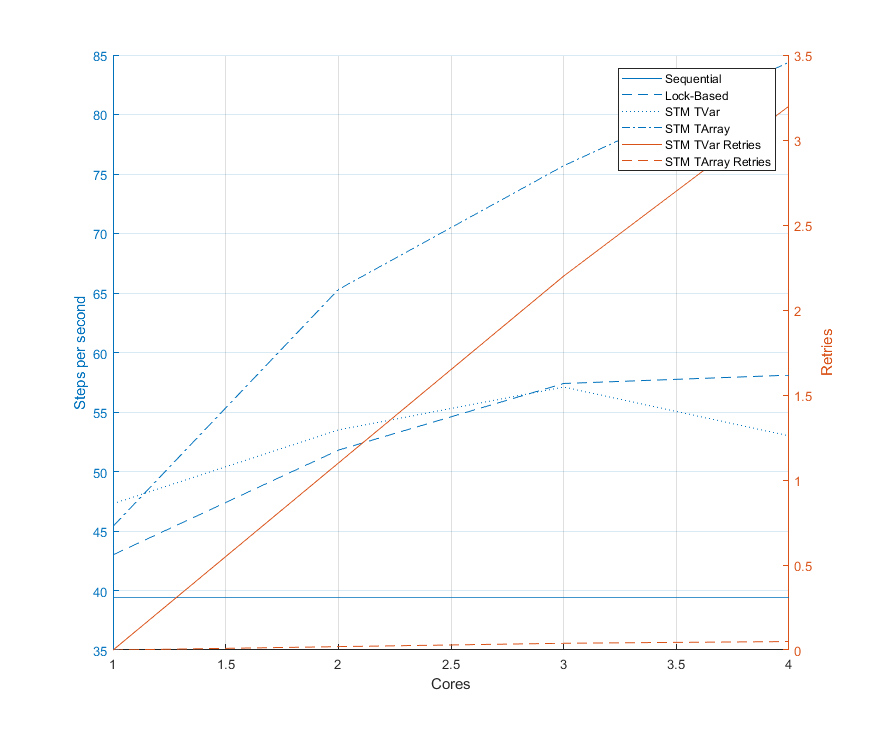
\includegraphics[width=0.7\textwidth, angle=0]{./fig/concurrentabs/sugarscape/varying_cores.png}
	\caption{Steps per second and retries on 50x50 grid and 500 initial agents on varying cores.}
	\label{fig:varying_cores}
\end{figure}

As expected, the \textit{Sequential} implementation is the slowest, followed by the \textit{Lock-Based} and \textit{TVar} approach whereas \textit{TArray} is the best performing one.

We clearly see that using a \textit{TVar} to share the environment is a very inefficient choice in this model: \textit{every} write to a cell leads to a retry independent whether the reading agent reads that changed cell or not, because the data-structure can not distinguish between individual cells. By using a \textit{TArray} we can avoid the situation where a write to a cell in a far distant location of the environment will lead to a retry of an agent which never even touched that cell. Also the \textit{TArray} seems to scale up by 10 steps per second for every core added. It will be interesting to see how far this could go with the Amazon experiment, as we seem not to hit a limit with 4 cores yet.

The inefficiency of \textit{TVar} is also reflected in the nearly similar performance of the \textit{Lock-Based} implementation which even outperforms it on 4 cores. This is due to very similar approaches because both operate on the whole environment instead of only the cells as \textit{TArray} does. This seems to be a bottleneck in \textit{TVar} reaching the best performance on 3 cores, which then drops on 4 cores due to an increasing retries ratio. The \textit{Lock-Based} approach seems to reduce its returns on increased number of cores hitting a limit at 4 cores as well.

\subsection{Scaling up Agents}
So far we kept the initial number of agents at 500, which due to the model specification, quickly drops and stabilises around 200 due to the carrying capacity of the environment as described in the book \cite{epstein_growing_1996} section \textit{Carrying Capacity} (p. 30).

We now want to measure the performance of our approaches under increased number of agents. For this we slightly change the implementation: always when an agent dies it spawns a new one which is inspired by the ageing and birthing feature of Chapter III in the book \cite{epstein_growing_1996}. This ensures that we keep the number of agents roughly constant (still fluctuates but doesn't drop to low levels) over the whole duration. This ensures a constant load of concurrent agents interacting with each other and demonstrates also the ability to terminate and create concurrent agents (threads) dynamically during the simulation.

Except for the \textit{Sequential} approach we ran all experiments with 4 cores (TVar with 3 as well). We looked into the performance of 500, 1,000, 1,500, 2,000 and 2,500 (maximum possible capacity of the 50x50 environment). The results are reported in Table \ref{tab:state_results_agentsscale_time} and plotted in Figure \ref{fig:state_results_agentsscale_time}.

\begin{table}
	\centering
  	\begin{tabular}{ c || c | c | c | c | c }
        Agents  & Sequential & Lock-Based & TVar (3 cores) & TVar (4 cores) & TArray  \\ \hline \hline 
    	    500     & 14.4       & 20.2		  &	20.1           & 18.5       	& \textbf{71.9}    \\ \hline
   		1,000   & 6.8        & 10.8 	      & 10.4           & 9.5         & \textbf{54.8}    \\ \hline
   		1,500   & 4.7        & 8.1 		  & 7.9            & 7.3			& \textbf{44.1}    \\ \hline
   		2,000   & 4.4        & 7.6 		  & 7.4            & 6.7    		& \textbf{37.0}    \\ \hline 
   		2,500   & 5.3        & 5.4 		  & 9.2            & 8.9			& \textbf{33.3}    \\ \hline \hline
   	\end{tabular}
  	
  	\caption{Steps per second on 50x50 grid with varying number of agents with 4 (and 3) cores except Sequential (1 core).}
	\label{tab:state_results_agentsscale_time}
\end{table}

\begin{figure}
	\centering
	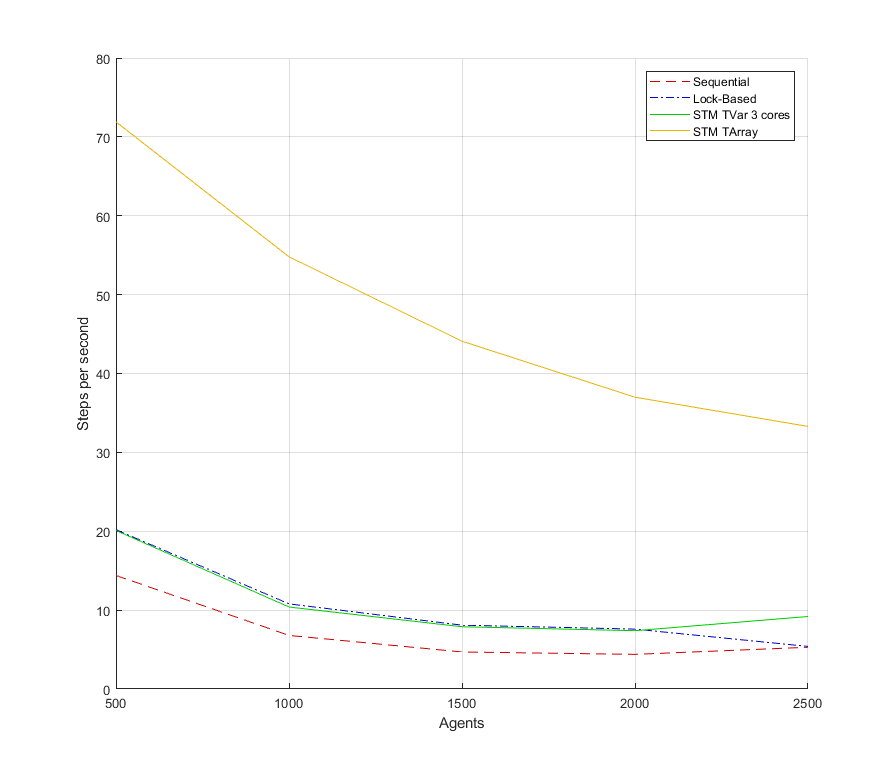
\includegraphics[width=1.0\textwidth, angle=0]{./fig/concurrentabs/sugarscape/varying_agents.png}
	\caption{Steps per second on 50x50 grid and varying number of agents with 4 (and 3) cores except Sequential (1 core).}
	\label{fig:state_results_agentsscale_time}
\end{figure}

As expected, the \textit{TArray} implementation outperforms all others substantially. Also as expected, the \textit{TVar} implementation on 3 cores is faster than on 4 cores as well when scaling up to more agents. The \textit{Lock-Based} approach performs about the same as the \textit{TVar} on 3 cores because of the very similar approaches: both access the \textit{whole} environment. Still the \textit{TVar} approach uses one core less to arrive at the same performance, thus strictly speaking outperforming the \textit{Lock-Based} implementation.

What seems to be very surprising is that in the \textit{Sequential} and \textit{TVar} cases the performance with 2,500 agents is \textit{better} than the one with 2,000 agents. The reason for this is that in the case of 2,500 agents, an agent can't move anywhere because all cells are already occupied. In this case the agent won't rank the cells in order of their pay-off (max sugar) to move to but just stays where it is. We hypothesize that due to Haskells laziness the agents actually never look at the content of the cells in this case but only the number which means that the cells themselves are never evaluated which further increases performance. This leads to the better performance in case of \textit{Sequential} and \textit{TVar} because both exploit laziness.
In the case of the \textit{Lock-Based} approach we still arrive at a lower performance because the limiting factor are the unconditional locks. In the case of the \textit{TArray} approach we also arrive at a lower performance because it seems that STM perform reads on the neighbouring cells which are not subject to lazy evaluation. In Haskell it is notoriously difficult to reason about efficiency (see Chapter \ref{ch:drawbacks} for a short discussion on drawbacks) and this behaviour of improved performance due to Haskells lazyness is no exception. We leave an in-depth investigation for further research as it is beyond the focus of this chapter.

We also measured the average retries both for \textit{TVar} and \textit{TArray} under 2,500 agents where the \textit{TArray} approach shows best scaling performance with 0.01 retries whereas \textit{TVar} averages at 3.28 retries. Again this can be attributed to the better transactional data-structure which reduces retry-ratio substantially to near-zero levels.

\subsection{Going Large-Scale}
To test how far we can scale up the number of cores in both the \textit{Lock-Based} and \textit{TArray} cases, we ran the two experiments (carrying capacity and rebirthing) on Amazon EC2 instances with increasing number of cores starting with 16 and 32 to see if we run into decreasing returns. The results are reported in Table \ref{tab:sug_varying_cores_amazon}.

\begin{table}
	\centering
%  	\begin{tabular}{ c || c | c | c }
%                   & Cores & Carrying Capacity & Rebirthing  \\ \hline \hline 
%    	Lock-Based & 16    & 53.9              & 4.4         \\ \hline
%    	Lock-Based & 32    & 44.2              & 3.6         \\ \hline \hline 
%   		
%   		STM TArray & 16    & \textbf{116.8} (0.23)      & \textbf{39.5} (0.08) \\ \hline
%   		STM TArray & 32    & 109.8 (0.41)      & 31.3 (0.18) \\ \hline \hline 
%   	\end{tabular}
  	
	\begin{tabular}{cc|c|c}
		\multicolumn{1}{ c||  }{\multirow{2}{*}{} } &
		\multicolumn{1}{ |c| }{Cores} & Carrying Capacity    & Rebirthing       \\ \hline \hline 
		
		\multicolumn{1}{ c||  }{\multirow{2}{*}{Lock-Based} } &
		\multicolumn{1}{ |c| }{16} & 53.9              & 4.4       \\ \cline{2-4}
		\multicolumn{1}{ c||  }{}                       &
		\multicolumn{1}{ |c| }{32} & 44.2              & 3.6      \\ \hline \hline 
		
		\multicolumn{1}{ c||  }{\multirow{2}{*}{STM TArray} } &
		\multicolumn{1}{ |c| }{16} & \textbf{116.8} (0.23)      & \textbf{39.5} (0.08)       \\ \cline{2-4}
		\multicolumn{1}{ c||  }{}                       &
		\multicolumn{1}{ |c| }{32} & \textbf{109.8} (0.41)      & \textbf{31.3} (0.18)      \\ \hline \hline 
	\end{tabular}  	
  	
  	\caption{Steps per second on varying cores on Amazon S2 Services.}
	\label{tab:sug_varying_cores_amazon}
\end{table}

As expected, the \textit{Lock-Based} approach doesn't scale up to many cores because each additional core brings more contention to the lock, resulting in even more decreased performance. This is particularly obvious in the rebirthing experiment because of the much larger number of concurrent agents. The \textit{TArray} approach returns better performance on 16 cores but fails to scale further up to 32 where the performance drops below the one with 16 cores. We indicated the retry-ratio in brackets and see that they roughly double from 16 to 32, which is the reason why performance drops as at this point. 

%the INCREASE in time can only happen due to more retries
%Carrying Capacity 16 core ~ 0.23 retry-ratio
%Carrying Capacity 32 core ~ 0.41 retry-ratio
%
%Rebirthing 16 core ~ 0.08 retry-ratio
%Rebirthing 32 core ~ 0.18 retry-ratio

\subsection{Comparison with other approaches}
The paper \cite{lysenko_framework_2008} reports a performance of 17 steps in RePast, 18 steps in MASON (both non-parallel) and 2,000 steps per second on a GPU on a 128x128 grid. Although our \textit{Sequential} implementation, which runs non-parallel as well, outperforms the RePast and MASON implementations of \cite{lysenko_framework_2008}, one must be very well aware that these results were generated in 2008, on current hardware of that time.

%When we run the SugarScape example of RePast with the same model parameters as ours on the same machine (see Table \ref{tab:machine_specs}) we arrive at roughly 450 steps per second - a factor of about 3.8 faster than even our STM \textit{TArray} implementation on 16 cores. This might seem quite shocking, even more so because RePast also performs visual output, rendering the SugarScape in every step. When scaling up the agents to 2,500 the RePast version arrives around roughly 95 steps per second which is still faster by a factor of 3 than our 4 core \textit{TArray} implementation. We attribute this substantial performance difference to the inherent performance difference of functional programming to imperative approaches as already outlined in the previous section. 

The very high performance on the GPU does not concern us here as it follows a very different approach than ours. We focus on speeding up implementations on the CPU as directly as possible without locking overhead. When following a GPU approach one needs to map the model to the GPU which is a delicate and non-trivial matter. With our approach we show that speed up with concurrency is very possible without the low-level locking details or the need to map to GPU. Also some features as bilateral trading between agents, where a pair of agents needs to come to a conclusion over multiple synchronous steps, is difficult to implement on a GPU whereas this is easily possible using STM.

Note that we kept the grid-size constant because we implemented the environment as a single agent which works sequentially on the cells to regrow the sugar. Obviously this doesn't really scale up on parallel hardware and experiments which we haven't included here due to lack of space, show that the performance goes down dramatically when we increase the environment to 128x128 with same number of agents which is the result of Amdahl's law where the environment becomes the limiting factor of the simulation. Depending on the underlying data-structure used for the environment we have two options to solve this problem. In the case of the \textit{Sequential} and \textit{TVar} implementation we build on an indexed array, which we can be updated in parallel using the existing data-parallel support in Haskell. In the case of the \textit{TArray} approach we have no option but to run the update of every cell within its own thread. We leave both for further research as it is out of scope of this paper.

\subsection{Discussion}
This case study showed clearly that besides being substantially faster than the \textit{Sequential} implementation, \textit{STM} is also able to perform considerably better than a \textit{Lock-Based} approach even in the case of a model with much higher complexity in agent behaviour and dramatically increased number of writes to the environment.
Further, this case study demonstrated that the selection of the right transactional data-structure is of fundamental importance when using \textit{STM}. Selecting the right transactional data-structure is very model-specific and can lead to dramatically different performance results.
In this case the \textit{TArray} performed best due to many writes but in the SIR case-study a \textit{TVar} showed good enough results due to the very low number of writes. When not carefully selecting the right transactional data-structure which supports fine-grained concurrency, a lock-based implementation might perform as well or even outperform the STM approach as can be seen when using the \textit{TVar}.
Although the \textit{TArray} is the better transactional data-structure overall, it might come with an overhead, performing worse on low number of cores than a \textit{TVar} approach but has the benefit of quickly scaling up to multiple cores. Depending on the transactional data-structure, scaling up to multiple cores hits a limit at some point. In the case of the \textit{TVar} the best performance is reached with 3 cores. With the \textit{TArray} we reached this limit around 16 cores.

Note that the comparison between the \textit{Lock-Based} approach and the \textit{STM TArray} implementation is a bit unfair due to a very different locking structure. A more suitable comparison would have been to use an indexed Array with a tuple of (MVar, IORef) in each cell to support fine-grained locking on cell-level. This would be a more just comparison to the \textit{STM Array} where fine-grained transactions happen on the cell-level. We hypothesize that \textit{STM} will still outperform the \textit{IO} approach but to a lesser degree - we leave the proof of this for further research.

%Unfortunately, for this model the performance is nowhere comparable to imperative approaches, which we attribute to the inherent performance difference of functional programming to imperative approaches. With the use of advanced language features we might arrive at much improved performance but we leave this for further research as we focus primarily on the comparison between lock-based and STM approaches.

%we can implement everything except synchronous direct agent-interactions atm: if agent-interaction is one-way e.g. paying back a loan then this is no problem. thus the following parts of the Sugarscape are not possible with our current STM approach: mating, trading and lending  because all 3 require direct agent-to-agent interaction over multiple steps. We leave the problem of developing such an algorithm / implementation for further research.

\subsection{Dynamic agent creation and removal}
Some models of ABS in general and Sugarscape in particular require the dynamic creation and removal of agents during simulation. The specific requirements here are that the agents themselves must be able to both remove themselves from the simulation and create new agents with given attributes. To achieve that, in such a simulation the output type of an agent must be richer than the one in the event-driven SIR. First, we define the output of an agent:

\begin{HaskellCode}
data AgentOut m e o = AgentOut
  { aoKill   :: Any              -- True if this agent should be removed 
  , aoCreate :: [AgentDef m e o] -- a list of agents to create
  , aoEvents :: [(AgentId, e)]   -- a list of events (receiver, event)
  }
\end{HaskellCode}

Note that \textit{AgentOut} contains already the list of scheduled events, which makes it clear that scheduling of events in this approach is implemented different than in the event-driven SIR, where the agents Monad stack had a \textit{WriterT} to write events to. The reason for that is that we treat agent-local abstractions different here because of the need to encapsulate local agent state as explained in subsequent sections.

If the agent wants to remove itself from the simulation, it simply sets \textit{aoKill} to True; if it wants to create new agents it adds an agent definition \textit{AgentDef} to the \textit{aoCreate} list. The agent definition \textit{AgentDef} holds the new id of the agent \footnote{Note that an agent-controlled id makes it possible to re-use ids in case an agent dies and in case ids have no other purposes than identifying event receivers in a model}, the MSF of the agent to create and the initial output of the new agent, so it has a representation in the visual or textual output for the current step without the need to run the new agent.

\begin{HaskellCode}
data AgentDef m e o = AgentDef
  { adId      :: AgentId         -- unique agent-id
  , adMSF     :: AgentMSF m e o  -- the agent behaviour function
  , adInitOut :: o               -- the value of the initial output
  }
\end{HaskellCode}

Further, the simulation must provide a \textit{global} mechanism to create new, unique \textit{AgentId} for the newly created agents. The generating of ids for the new agents have to occur within the parent agents themselves because in some models they might need this very id to communicate with their children - an indirection through the kernel would only complicate matters. We thus start with a data definition, holding the next agent id - if an agent creates a new agent it simply reads that value and increments it by 1.

\begin{HaskellCode}
data ABSState = ABSState { absNextId :: AgentId }
\end{HaskellCode}

To make it \textit{globally} available to all agents a \textit{StateT ABSState} Monad transformer is used, which is also the innermost Monad of the Monad stack of Sugarscape \footnote{In the Sugarscape implementation, \textit{ABSState} also holds the current simulation time, which is omitted here for clarity reasons.}.

\begin{HaskellCode}
type AgentMonad m = StateT ABSState m
\end{HaskellCode}

Finally, we can define the polymorphic type of the agent MSF, as it is used in Sugarscape, where it is parametrised with model specific types (see next sections). It is similar to the event-driven SIR, where the agent takes the \textit{ABSEvent} as input but the output is now a tuple of \textit{AgentOut} and the polymorphic agent output type \textit{o}. The reason why the output type \textit{o} is not part of \textit{AgentOut} is to keep \textit{AgentOut} a Monoid, which allows accumulative / iterative change to \textit{AgentOut}, which is important for creating new agents and scheduling events, as explained in the agent-local abstractions below.

\begin{HaskellCode}
type AgentMSF m e o = MSF (AgentMonad m) (ABSEvent e) (AgentOut m e o, o)
\end{HaskellCode}

\subsection{Shared Mutable Proactive Environment}
In many agent-based models, agents are placed on a discrete 2D grid environment and can move around and interact with the environment. Often, there exist specific constraints. For example, that each position can only be occupied by one agent at most. This restriction requires specific iteration semantics, which make it impossible that two agents end up at the same time in the same spot. In general, such models solve this problem by using the sequential strategy as described in Chapter \ref{sec:seq_strategy}, where agents are run in random order, one after another. This allows the agents to access the globally shared, mutable environment exclusively when it is their turn and they interact and change it without the danger of other agents interfering.

To implement a shared, mutable and proactive environment, first we define a generic discrete 2D grid environment with polymorphic cells. The selection of the right data structure is crucial. Initially we used an \texttt{IArray} from the \href{http://hackage.haskell.org/package/array}{array library}~\cite{array_hackage}. This data structure has excellent read performance, but in performance tests we experienced serious performance and memory leak issues with updates. This issue lead to allocation of about 40 MByte per second on our hardware. Clearly this is unacceptable for simulation purposes, where software often runs for hours and requires memory consumption to stay within reasonable bounds. The solution was to switch to \texttt{IntMap} from the \href{http://hackage.haskell.org/package/containers}{container's library}~\cite{containers_library} as an underlying data structure which solved both the performance and memory leak issues.

\begin{HaskellCode}
type Discrete2dCoord  = (Int, Int)
type Discrete2dCell c = (Discrete2dCoord, c)
type Discrete2d c     = Map.IntMap (Discrete2dCell c)
\end{HaskellCode}

Having introduced the \texttt{AgentMSF} and fixed the \texttt{AgentMonad} with the \texttt{StateT ABSState} as the outermost Monad, adding a globally shared, mutable environment is straightforward. The solution is to simply add another \texttt{StateT} Transformer with the given environment as type. Below, we give the parametrised definition as in the Sugarscape implementation. Sugarscape closes the Monad stack with the \texttt{Rand} Monad as stochastics play an important role in the Sugarscape model as well. Therefore, a full expansion of the Monad stack used in Sugarscape is \texttt{StateT ABState (StateT SugEnvironment (Rand g))}.

\begin{HaskellCode}
data SugEnvSite = SugEnvSite 
  { sugEnvSiteSugarLevel    :: Double
  , sugEnvSiteSpiceLevel    :: Double
  , sugEnvSitePolutionLevel :: Double
  ...
  }

type SugEnvironment  = Discrete2d SugEnvSite
type SugAgentMonad g = AgentMonad (StateT SugEnvironment (Rand g))
\end{HaskellCode}

When implementing the proactivity of the environment, we must make a clear distinction between the environment's data structure, how agents access it, and the environment's behaviour. In the Sugarscape model, the behaviour of the environment is quite trivial, as it simply regrows resources over time and diffuses pollution in case the pollution is turned on. This behaviour is achieved by providing a pure function without any monadic context or \texttt{MSF}. This is not necessary because the environment, as we implement it, does not encapsulate local state and it does not interact with agents through messages and vice versa. Thus, a pure function of type \texttt{Time $\rightarrow$ SugEnvironment $\rightarrow$ SugEnvironment}, which maps the environment to the environment over time is enough for our purpose. It also takes the current simulation time so it can implement seasons, where the speed of regrowth of resources is different in different regions and swaps after some time. This function is called in the simulation kernel after every \texttt{Tick}.

\medskip

Generally, one can distinguish between four different types of environments in ABS:

\begin{enumerate}
	\item \textit{Passive Read Only} - Implemented in Chapter \ref{sec:adding_env}, where the environment itself is not modelled as an active process and is static information, for example, a list of neighbours, passed to each agent. The agents cannot change the environment actively and in the case of Chapter \ref{sec:adding_env}, this is enforced at compile time by simply making it read only, by including it in the input but not the output type of an agent. The agents change the environment implicitly by changing their state, but there is no notion of an active environment process.
	
	\item \textit{Passive Read and Write} - The environment is just shared data, which can be accessed and manipulated by the agents. This situation forces some arbitration mechanism to prevent conflicting updates. An example for preventing these updates would be running the agents sequentially one after the other, to ensure that only one agent has access at a time.
	
	\item \textit{Active Read and Write} - As implemented above. To make it active a pure function is used where the environment data is owned by the simulation kernel and then made available to the agents through a \texttt{State} Monad. Another approach would be to implement the environment process as an agent, which is run together with all the other agents. This allows the environment to send and receive messages but the guarantees about when the environment will be run is lost if agents are run sequentially in random order.
	
	\item \textit{Active Read Only} - Can be implemented as above but instead of providing the environment data through a \texttt{State} Monad, a \texttt{Reader} Monad is used. The environment data is owned by the simulation kernel and the process runs as a pure function as before, but the data is provided in a read only way through the \texttt{Reader} Monad. The same can also be achieved by passing it as input only to the agent as was done in Chapter \ref{sec:adding_env}.
\end{enumerate}

\subsection{Agent-Local Abstractions}
After having established Sugarscape's full Monad stack, we can now move on to specify the agent behaviour and develop advanced agent-local concepts and abstractions. Before we can parametrise the \texttt{AgentMSF}, we need to define model-specific data definitions for the event type \texttt{e} and the output type \texttt{o}. Thus, we define the event type \texttt{SugEvent}, which defines all the event types of Sugarscape and the output type \texttt{SugAgentObservable}, which contains all observable properties, an agent wants to communicate to the outside world, for visualisation or exporting purposes. 

\begin{HaskellCode}
data SugEvent = MatingRequest AgentGender
              | MatingReply 
                 (Maybe (Double, Double, Int, Int, CultureTag, ImmuneSystem))
              ...

data SugAgentObservable = SugAgentObservable
  { sugObsSugMetab :: Int     -- metabolism
  , sugObsSugLvl   :: Double  -- sugar wealth
  , sugObsAge      :: Int     -- current age
  ...  
  }
\end{HaskellCode}

We can now parametrise the \texttt{AgentMSF} with the right types for the Sugarscape model.

\begin{HaskellCode}
type SugAgentMSF g = AgentMSF (SugAgentMonad g) SugEvent SugAgentObservable
\end{HaskellCode}

Next, we define the type of the top-level agent behaviour function. We want to make the unique agent id and the model configuration (scenario) explicit, so it will be passed as curried arguments to the function. Furthermore, the initial agent state is passed as curried input as well.

\begin{HaskellCode}
data SugarScapeScenario = SugarScapeScenario 
  { sgScenarioName    :: String
  , sgPollutionActive :: Bool
  ...
  }

data SugAgentState = SugAgentState
  { sugAgSugarMetab :: Int     -- metabolism
  , sugAgVision     :: Int     -- vision in all four directions
  , sugAgSugarLevel :: Double  -- sugar wealth
  , ...
  }
  
type SugarScapeAgent g 
       = SugarScapeScenario -> AgentId -> SugAgentState -> SugAgentMSF g
\end{HaskellCode}

Now we have fully specified types for the Sugarscape agent. The types indicate very clearly the intention and the interface. What is of high importance is that we don't have any impure \texttt{IO} monadic context anywhere in our type definitions and we can also guarantee that it will not somehow sneak in. The transformer stack of the agents \texttt{MSF} is closed through the \texttt{Rand} Monad, consequently it is simply not possible to add other layers. 

An agent is fully represented by a top level \texttt{SugarScapeAgent} function, which encapsulates the whole agent behaviour. Next we will look at how to define agent-local behaviour, which is hidden behind the \texttt{SugarScapeAgent} function type. Whereas the previously defined types are exposed to the whole simulation, the following section deals with types and behaviour which are locally encapsulated and hidden from the simulation kernel. In the next sections we show how to encapsulate the agents' state locally while retaining mutability. Further, we explain how sending of events works in the Sugarscape implementation and how to achieve read-only access to the agents unique id and the model configuration.

\subsubsection{Agent-local state}
To implement the local encapsulation of the agents' state is straightforward with MSFs as they are continuations, allowing them to capture local data using closures. Fortunately we do not need to implement the low-level plumbing, as Dunai provides us with the suitable function \texttt{feedback :: Monad m $\Rightarrow$ c $\rightarrow$ MSF m (a, c) (b, c) $\rightarrow$ MSF m a b}. It takes an initial value of type \texttt{c} and an \texttt{MSF} which takes in addition to its input \texttt{a} also the given type \texttt{c} and outputs in addition to type \texttt{b} also the type \texttt{c}, which clearly indicates the read and write property of type \texttt{c}. The function returns a new \texttt{MSF} which only operates on \texttt{a} as input and returns \texttt{b} as output by running the provided \texttt{MSF} and feeding back the \texttt{c} (with the initial \texttt{c} at the first call).

\begin{HaskellCode}
sugarscapeAgent :: RandomGen g => SugarScapeAgent g
sugarscapeAgent scen aid s0 = feedback s0 (proc (evt, s) -> do ... )
\end{HaskellCode}

Before we can move on to write a function handling incoming events, we need to define the \textit{agent-local} Monad stack. The event handler must be able to manipulate the agent-local state we just encapsulated through \texttt{feedback}, support reading the unique agent id and model scenario and scheduling of events.

Providing the local, mutable agent state is done using a \texttt{State} Monad. Providing the model configuration (scenario) and the unique agent id is done using the \texttt{Reader} Monad. For implementing event scheduling, a \texttt{Writer} Monad is used, which is the same mechanism as in the event-driven SIR. As the Monoid type for \texttt{WriterT}, the \texttt{AgentOut} is used. All fields of its data definition are Monoid instances, making \texttt{AgentOut} a Monoid as well, thus writing a type class instance for it is trivial. This approach allows to easily add new agent definitions and mark an agent for removal throughout the agents behaviour. Further, it is simple to send new events through \texttt{AgentOut} as it contains the list of events, as discussed in the previous section \ref{sec:dynamic_creationremoval}. Having established this, we define the agent local Monad which is only used \textit{within} \texttt{AgentMSF}.

\begin{HaskellCode}
type AgentLocalMonad g = WriterT (SugAgentOut g) 
                           (ReaderT (SugarScapeScenario, AgentId) 
                             (StateT SugAgentState (SugAgentMonad g)))     
-- FULLY EXPANDS TO:
-- WriterT (SugAgentOut g) 
--  (ReaderT (SugarScapeScenario, AgentId) 
--    (StateT SugAgentState 
--      (StateT ABSState 
--        (StateT SugEnvironment 
--          (Rand g)))))
\end{HaskellCode}

Now we can define the \texttt{MSF} which handles an event. It has the \texttt{AgentLocalMonad} monadic context, takes an \texttt{ABSEvent} parametrised over \texttt{SugEvent} (it has also to handle \texttt{Tick}). What might come as a surprise is that it returns unit type, implying that the results of handling an event are only visible as side effects in the Monad stack. This is intended. We could pass all arguments explicitly as input and output but that would complicate the handling code substantially, thus we opted for a monadic, imperative style handling of events.

\begin{HaskellCode}
type EventHandler g = MSF (AgentLocalMonad g) (ABSEvent SugEvent) ()
\end{HaskellCode}

To run the handler within the \texttt{SugarScapeAgent}, we make use of Dunai's functionality which provides functions to run MSFs with additional monadic layers within MSFs. We use \texttt{runStateS}, \texttt{runReaderS} and \texttt{runWriterS} (\texttt{S} indicates the stream character) to run the \texttt{generalEventHandler}, providing the initial values for the respective Monads, \texttt{s} for the \texttt{StateT}, \texttt{(params, aid)} for the \texttt{ReaderT} and the \texttt{evt} as the input to the event handler. \texttt{WriterT} does not need an initial value, it will be provided through the Monoid instance of \texttt{AgentOut}.

\begin{HaskellCode}
sugarscapeAgent :: RandomGen g => SugarScapeAgent g
sugarscapeAgent scen aid s0 = feedback s0 (proc (evt, s) -> do
  (s', (ao', _)) <- runStateS 
                      (runReaderS 
                        (runWriterS generalEventHandler)) -< (s, ((scen, aid), evt))
  let obs = sugObservableFromState s
  returnA -< ((ao', obs), s'))

sugObservableFromState :: SugAgentState -> SugAgentObservable
generalEventHandler :: RandomGen g => EventHandler g
\end{HaskellCode}

Now it is also clear why the output of an agent is a tuple of \texttt{AgentOut} and the polymorphic type \texttt{o}: the latter one is parametrised to \texttt{SugAgentObservable}, which is not constructed through the use of \texttt{WriterT} but simply a projection of the agent state through \texttt{sugObservableFromState}. In the next section we explain the details of \texttt{generalEventHandler}, which implements the main event handling mechanisms of an agent.

\subsubsection{Handling and sending of events}
Now we are ready to implement handling of events on an agent-local level: we receive the events from the simulation kernel as input and run within a six-layered Monad Transformer stack which is partly global, controlled by the simulation kernel, and partly local to the agent, controlled by the agent itself. The layers are the following (inner to outer):

\begin{enumerate}
	\item \texttt{WriterT (SugAgentOut g)} - local; provides write-only functionality for constructing the agent output for the simulation kernel communicating whether to kill the agent, a list of new agents to create and a list of events to send to receiving agents.
	
	\item \texttt{ReaderT (SugarScapeScenario, AgentId)} - local; provides the read-only model configuration and unique agent id.

	\item \texttt{StateT SugAgentState} - local; provides the local mutable agent state.

	\item \texttt{StateT ABSState} - global; provides unique agent ids for new agents. %and the current simulation time. The usage of a \textit{StateT} is slightly flawed here because it provides too much power: the current simulation time should be read-only to the agent. Drawing the next agent-id involves reading the current id and writing the incremented value, thus technically it is a \textit{StateT} but ideally we would like to hide the writing operation and only provide a \textit{read-current-and-increment} operation. A possible solution would be to provide the current simulation time through a \textit{ReaderT} and the new agent-id through a new monad which uses the \textit{StateT} under the hood, like the \textit{Rand} monad.

	\item \texttt{StateT SugEnvironment} - global; provides the Sugarscape environment which the agents can read and write.

	\item \texttt{Rand g} - global; provides the random-number stream for all agents.
\end{enumerate}

Finally we can implement the event handler \texttt{generalEventHandler}, which simply matches on the incoming events, extracts data and dispatches to respective handlers. What is crucial here to understand is that only the top level \texttt{sugarscapeAgent} and the \texttt{EventHandler} function are MSFs which simply dispatch to monadic functions, implementing the functionality in an imperative programming style. The main benefit of the MSFs are their continuation character, which allows to encapsulate local state. An additional benefit of MSFs is that the  Dunai library adds a lot of additional functionality of composing MSFs and running different monadic context on top of each other. It even provides exception handling through MSFs with the \texttt{Maybe} type, thus programming with exceptions in ABS models can be done as well. We didn't make use of exceptions, as the Sugarscape model simply does not specify any exception handling on the model level and there was also no opportunity to use exceptions from which to recover on a technical level \footnote{There are exceptions on a technical level but they are non-recoverable and should never occur at runtime, thus the function \texttt{error} is used, which terminates the simulation with an error message.}.

\begin{HaskellCode}              
generalEventHandler :: RandomGen g => EventHandler g
generalEventHandler =
  continueWithAfter -- optionally switching the top event handler 
    (proc evt -> 
      case evt of 
        Tick dt -> do
          mhdl <- arrM handleTick -< dt
          returnA -< ((), mhdl)

        (DomainEvent sender (MatingRequest otherGender)) -> do
          arrM (uncurry handleMatingRequest) -< (sender, otherGender)
          returnA -< ((), Nothing)
        ...)
        
handleTick :: RandomGen g => DTime -> AgentLocalMonad g (Maybe (EventHandler g))
handleMatingRequest :: AgentId -> AgentGender -> AgentLocalMonad g ()
\end{HaskellCode}

The use of \texttt{continueWithAfter} is a customised version of the already known \texttt{switch} combinator. It allows to swap out the event-handler for a different one, which is the foundation for the synchronous agent interactions, as discussed in the next section.

To see how an event handler works, we provide the implementation of \\ \texttt{handleMatingRequest}. It is sent by an agent to its neighbours to request whether they want to mate with this agent. The handler receives the sender and the other agents gender and replies with \texttt{sendEventTo} which sends a \texttt{MatingReply} event back to the sender. The function \texttt{sendEventTo} operates on the \texttt{WriterT} to append (using \texttt{tell}) an event to the list of events this agent sends when handling this event. The use of \texttt{agentProperty} reads the value of a given field of the local agent state. 

\begin{HaskellCode}
handleMatingRequest :: AgentId
                    -> AgentGender
                    -> AgentLocalMonad g ()
handleMatingRequest sender otherGender = do
  -- check if the agent is able to accept the mating request: 
  -- fertile + wealthy enough + different gender
  accept <- acceptMatingRequest otherGender
  -- each parent provides half of its sugar-endowment for the new-born child
  acc <- if not accept
      -- can't mate, simply send Nothing in MatingReply
      then return Nothing
      else do
        sugLvl  <- agentProperty sugAgSugarLevel
        spiLvl  <- agentProperty sugAgSpiceLevel
        metab   <- agentProperty sugAgSugarMetab
        vision  <- agentProperty sugAgVision
        culTag  <- agentProperty sugAgCultureTag
        imSysGe <- agentProperty sugAgImSysGeno -- immune system genotype
        -- able to mate, send Just share in MatingReply
        return Just (sugLvl / 2, spiLvl / 2, metab, vision, culTag, imSysGe)
  -- reply to sender with MatingReply
  sendEventTo sender (MatingReply acc)
\end{HaskellCode}

Finally, we have a look at how to actually run an agents' \texttt{MSF} using the function \texttt{runAgentMSF}. It is a \textit{pure} function as well and thus takes all input as explicit arguments. It might look like an excess to pass in five arguments and get a six-tuple as result but this is the price we have to pay for pure functional programming where everything is explicit, with all its benefits and drawbacks.

\begin{HaskellCode}
runAgentMSF :: RandomGen g        -- RandomGen type class for g
            => SugAgentMSF g      -- agents MSF to run.
            -> ABSEvent SugEvent  -- event it receives.
            -> ABSState           -- ABSState (next agent id and current time)
            -> SugEnvironment     -- environment state
            -> g                  -- random-number generator
            -> (SugAgentOut g, SugAgentObservable, SugAgentMSF g, 
                ABSState, SugEnvironment, g)
runAgentMSF msf evt absState env g = (ao, obs, msf', absState', env', g') 
  where
    -- extract the monadic function to run
    msfAbsState = unMSF msf evt
    -- peel away one State layer: ABSState
    msfEnvState = runStateT msfAbsState absState
    -- peel away the second State layer: SugEnvironment
    msfRand = runStateT msfEnvState env
    -- peel away the 3rd and last layer: Rand Monad
    (((((ao, obs), msf'), absState'), env'), g') = runRand msfRand g
\end{HaskellCode}

We run only the three \textit{global} monadic layers in here, the three \textit{local} layers are indeed completely local to the agent itself as shown above.

\subsection{Synchronous agent interactions}
With the concepts introduced so far we can achieve already a lot in terms of agent interactions: agents can react to incoming events, which are either the \textit{Tick} event advancing simulation time by one step or a message sent by another agent (or the agent itself). This is enough to implement simple one-directional agent interactions where one agent sends a message to another agent but does not await an answer within the same \textit{Tick}. This one-directional interactions is used in the model to implement the passing of diseases, the paying back of debt, passing on wealth to children upon death - the agent simply sends a message and forgets about it.

Unfortunately this mechanism is not enough to implement the other agent-interactions in the Sugarscape model, which are structurally richer: they need to be synchronous. In the use-cases of mating, trading and lending two agents need to come to an agreement over multiple interactions steps within the same \textit{Tick} which need to be exclusive and synchronous.  This means that an agent A initiates such a multi-step conversation with another agent B by sending an initial message to which agent B has to react by a reply to agent A who upon reception of the message, will pick up computation from that point and reply with a new message and so on. Both agents must not interact with other agents during this conversation to guarantee resource constraints, otherwise it would become quite difficult and cumbersome to ensure that agents don't spend more than they have when trading with multiple other agents at the same time. Also the initiating agent A must be able to pick up processing of its \textit{Tick} event from the point where it started the conversation with agent B because sending a message always requires the handling of the current event to exit and hand the control back to the simulation kernel. See Figure \ref{fig:syncagentinteractions} for a visualisation of the sequence of actions.

\begin{figure}
	\centering
	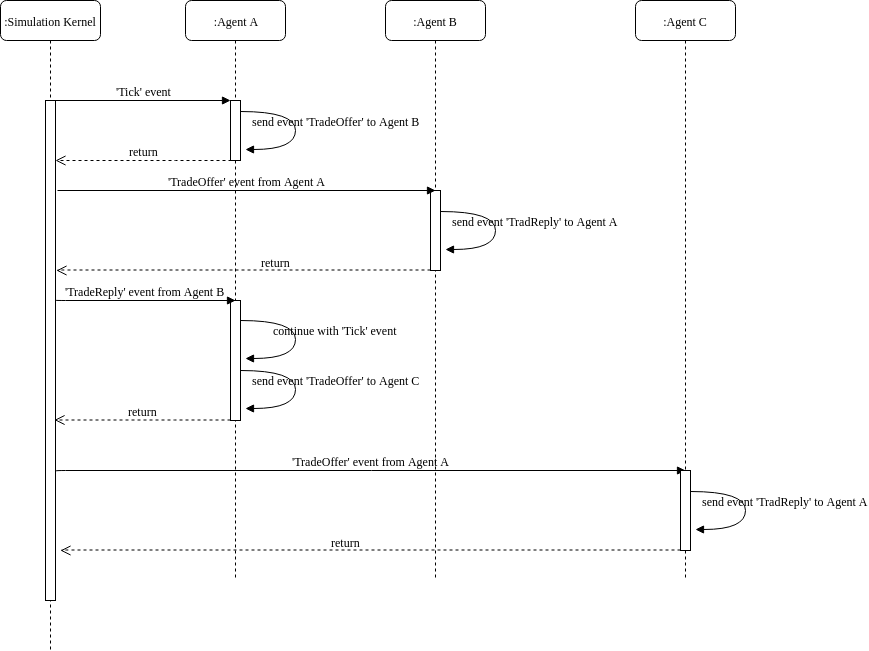
\includegraphics[width=1.0\textwidth, angle=0]{./fig/eventdriven/syncagentinteractions.png}
	\caption{Sequence diagram of synchronous agent interaction in the trading use-case. Upon the handling of the \textit{Tick} event, agent A looks for trading partners and finds agent B within its neighbourhood and sends a \textit{TradingOffer} message. Agent B replies to this message with \textit{TradeReply} and agent A continues with the trading algorithm by picking up where it has left the execution when sending the message to agent B. After agent A has finished the trading with agent B, it turns to agent C, where the same procedure follows.}
	\label{fig:syncagentinteractions}
\end{figure}

The way to implement this is to allow an agent to be able to change its internal event-handling state: to switch into different event-handlers, after having sent an event, to be able to react to the incoming reply in a specific way by encapsulating local state for the current synchronous interaction through closures and currying. Further, by making use of continuations the agent can pick up the processing of the \textit{Tick} event after the synchronous agent interaction has finished. Key to this is the function \textit{continueWithAfter} which we already shortly introduced through \textit{generalEventHandler}. This function takes an MSF which returns an output of type \textit{b} and an optional MSF. If this optional \textit{Maybe} MSF is \textit{Just} then the \textit{next} input is handled by this new MSF. In case no new MSF is returned (\textit{Nothing}), the MSF will stay the same. This is a more specialised version of the \textit{switch} combinator introduced in Chapter \ref{sec:back_frp} in the way that it doesn't need an additional function to produce the actual MSF continuation. Note that the semantics are different though: whereas \textit{switch} runs the new MSF immediately, \textit{continueWithAfter} only applies the new MSF in the \textit{next} step. The implementation of the function is as follows:

\begin{HaskellCode}
continueWithAfter :: Monad m => MSF m a (b, Maybe (MSF m a b)) -> MSF m a b
continueWithAfter msf = MSF (\a -> do
  ((b, msfCont), msf') <- unMSF msf a
  let msfNext = fromMaybe (continueWithAfter msf') msfCont
  return (b, msfNext))
\end{HaskellCode}

Finally, we can discuss the \textit{Tick} handling function. It returns a value of type \textit{Maybe (EventHandler g)} which if is \textit{Just} will result in to a change of the top-level event handler through \textit{continueWithAfter} as shown in \textit{generalEventHandler} above. Note the use of continuations in the case of \textit{agentMating, agentTrade} and  \textit{agentLoan}. All these functions return a \textit{Maybe (EventHandler g)} because all of them can potentially result in synchronous agent interactions which require to change the top-level event handler. The function \textit{agentDisease} is the last in the chain of agent behaviour, thus we are passing a default continuation which simply switches back into \textit{generalEventHandler} to finish the processing of a \textit{Tick} in an agent.

\begin{HaskellCode}
handleTick :: RandomGen g => DTime -> AgentLocalMonad g (Maybe (EventHandler g))
handleTick dt = do
  -- perform ageing of agent
  agentAgeing dt
  -- agent move, returns amount it of resources it harvested
  harvestAmount <- agentMove
  -- metabolise resources, depending on agents metabolism rate
  -- returns amount metabolised
  metabAmount <- agentMetabolism
  -- polute environment given harvest and metabolism amount
  agentPolute harvestAmount metabAmount

  -- check if agent has starved to death or died of age
  ifThenElseM
    (starvedToDeath `orM` dieOfAge)
    (do
      -- died of age or starved to deat: remove from simulation
      agentDies agentMsf
      return Nothing) 
    -- still alive, perform the remaining steps of the behaviour
    -- pass agentContAfterMating as continuation to pick up after mating
    -- synchronous conversations have finished
    (agentMating agentMsf agentContAfterMating)

-- after mating continue with cultural process and trading
agentContAfterMating :: RandomGen g => AgentLocalMonad g (Maybe (EventHandler g))
agentContAfterMating = do
    agentCultureProcess
    -- pass agentContAfterTrading as continuation to pick up after trading 
    -- synchronous conversations have finished
    agentTrade agentContAfterTrading 

-- after trading continue with lending and borrowing
agentContAfterTrading :: RandomGen g  => AgentLocalMonad g (Maybe (EventHandler g))
agentContAfterTrading = agentLoan agentContAfterLoan

-- after lending continue with diseases, which is the step in a Tick event
agentContAfterLoan :: RandomGen g => AgentLocalMonad g (Maybe (EventHandler g))
agentContAfterLoan = agentDisease defaultCont

-- safter diseases imply switch back into the general event handler
defaultCont :: RandomGen g => AgentLocalMonad g (Maybe (EventHandler g))
defaultCont = return (Just generalEventHandler)
\end{HaskellCode}

\subsubsection{Tagless final}
Although the indirect, continuation based approach to synchronous agent interactions as shown before works, it is quite cumbersome, fragile and it is easy to get something wrong. What would be more desirable is to have a truly synchronous approach, where the reply to an event happens directly as a result of the \textit{sendEventTo} function: when calling \textit{sendEventTo}, behind the scenes the receiving agent is executed and the result is returned directly to the caller, without any indirections. With the \textit{tagless final} approach as introduced in the event-driven SIR above, this becomes possible in an elegant and robust way. We have developed this concept for the event-driven SIR only. Still, it should be equally applicable for the Sugarscape but we leave that for further research.

We start by extending the API by defining a \textit{new} typeclass \textit{MonadAgentSync}:

\begin{HaskellCode}
class Monad m => MonadAgentSync e m | m -> e where
  sendSync :: e -> AgentId -> m (Maybe [e])
\end{HaskellCode}

The semantics behind the \textit{sendSync} method shall be that it allows to send an event of type \textit{e} to agent with id \textit{AgentId}. If the agent cannot be found it will return \textit{Nothing}, otherwise it will return \textit{Just} the list of events the receiving agent replies to the sending agent. 

The only place which has to be changed is the susceptible agent but due to the different semantics, parts of its behaviour needs to be rewritten. The receiving agents are left unchanged as at the moment a receiver has no means to distinguish between asynchronous and synchronous events and is not forced to reply to the sender in case of a synchronous event. It would be useful to have some mechanism that in case of a synchronous event, the receiver can only reply to the sender. We leave that issue for further research.

Handling an incoming \textit{Contact} from an \textit{Infected} is no longer necessary as it will not happen, because the interactions go directly through \textit{sendSync} and infected agents don't make contact pro-actively. Thus, the \textit{MakeContact} handler has to be changed to take into account that the infection can happen directly there:

\begin{HaskellCode}
handleEvent MakeContact = do
  ais        <- getAgentIds
  ai         <- getMyId
  isInfected <- makeContact beta ai ais
  if isInfected
    -- got infected, signal event to switch
    then return (Just ())
    else do
      -- not infected, re-schedule MakeContact
      scheduleMakeContact
      return Nothing
\end{HaskellCode}

The function \textit{makeContact} recursively \textit{makeContactWith} $\beta$ (contact rate) other agents. Whereas previously, sending a \textit{Contact} event to itself was not a problem, this is not allowed any more and must be prevented explicitly. The reason for that is discussed below in the implementation of the \textit{sendSync} method of the pure interpreter. Note that sending to itself counts against the $\beta$ contacts, as it would make no difference: receiving a \textit{Contact} from a \textit{Susceptible} has no effect on a susceptible agent anyway. If the case arises in a model that agents need to send events to themselves, it cannot happen through mechanisms like \textit{sendSync} but it has to go through asynchronous scheduling of events which decouples the sending from the receiving.

\begin{HaskellCode}
makeContact :: (MonadAgent SIREvent m, MonadAgentSync SIREvent m)
            => Int       -- ^ number of contacts to make
            -> AgentId   -- ^ sender agent id
            -> [AgentId] -- ^ all agent ids (including self)
            -> m Bool
makeContact 0 _ _ = return False
makeContact n ai ais = do
  receiver <- randomElem ais
  -- prevent sending to self
  if ai == receiver
    -- self counts against beta contacts
    then makeContact (n-1) ai ais
    else do
      -- make contact
      ret <- makeContactWith receiver
      if ret
        -- got infected, stop
        then return True
        -- not infected, continue
        else makeContact (n-1) ai ais
\end{HaskellCode}

Finally we can use \textit{sendSync} to directly send events to a receiving agent, which replies with a list of events to the sender. Note that we needed to add the new \textit{MonadAgentSync} typeclass to the overloaded function, to make the \textit{sendSync} method available.

\begin{HaskellCode}
makeContactWith :: (MonadAgent SIREvent m, MonadAgentSync SIREvent m) 
                => AgentId -> m Bool
makeContactWith receiver = do
  ai     <- getMyId
  -- DIRECT SYNCHRONOUS AGENT INTERACTION HAPPENS HERE
  retMay <- sendSync (Contact ai Susceptible) receiver
  case retMay of 
    -- receiver not found, no infection
    Nothing -> return False
    -- receiver found, replied with es events
    (Just es) -> do
      -- check if any event in replies is from Infected
      let fromInf = any (\ (Contact _ s) -> s == Infected) es
      if not fromInf
        -- none from Infected, no infection
        then return False
        -- at least one from Infected, might become infected
        else do
          r <- randomBool inf
          if r 
            -- got infected, become infected
            then do
              scheduleRecoveryM ild
              return True
            else return False
\end{HaskellCode}

The \textit{sendSync} method needs to be implemented in a new \textit{pure} interpreter, which follows exactly the same concept as before so we briefly discuss it conceptually. The method looks up the receiving agent, runs it with the given event of the sender and filters the replies to the sending agent. To do that, the method needs to have all agents available to actually execute them. This is achieved by keeping the agent mappings in the \textit{SimState}, introduced in the initial section on \textit{tagless final} of the event-driven SIR. They are managed using a \textit{State} Monad, thus can be read and written, which both is necessary as after a successful run of the receiving agent, its new MSF needs to be put back into the agent mappings.

Now it becomes clear why an agent cannot send an event with \textit{sendSync} to itself and why circular (agent A sendSync to agent B sendSync to agent C sendSync to agent A) \textit{sendSync} are also not allowed. The new MSF of an agent which was just run and updated in the \textit{SimState} will be overridden by the subsequent updates of runs which were initiated earlier. Fortunately, this can be conveniently checked within the \textit{sendSync} method and an error or exception can be generated which is better than silently ignoring it, resulting in unexpected behaviour. It is possible because the initiating agents id is always known and because it is easy to keep track of the agent ids currently engaged in a \textit{sendSync} by storing their ids in the \textit{SimState}, thus arriving at some kind of call stack management.

Although the very direct \textit{tagless final} agent interaction approach makes things under certain circumstances easier, it comes also with subtle drawbacks, thus it depends on the model semantics which approach to synchronous agent interactions should be chosen. Still we think that this approach is another demonstration of the usefulness of a \textit{tagless final} approach: we have shown how to extend the existing API with new operations without breaking the existing implementation. Also we think that we only scratched the surface with this approach of direct synchronous agent interactions but we leave a more in-depth exploration of it for further research.

%\section{Implementation Approaches}
5 Pages

This is now very programming-language specific

\begin{itemize}
	\item Mapping the strategies to 3 programming-languages: Java, Scala with Actors, Haskell
	\item Comparing the programming languages in regard of their suitability to implement each of these strategies
	\item Screen-shots of results of the same simulation-model with all the strategies
\end{itemize}

%\input{./tex/eventdriven/eventdrivenSIR.tex}

\section{Discussion}
Although there are similarities to the work of \cite{botta_time_2010} (the use of messages and the problem of when to advance time in models with arbitrary number synchronised agent-interactions), we approach our agents differently. First in our approach an agent is only a single MSF and thus can not be directly queried for its internal state / its id or outgoing messages, instead of taking a list of messages, our agents take a single event/message and can produce an arbitrary number of outgoing messages together with an observable state - note that this would allow to query the agent for its id and its state as well by simply sending a corresponding message to the agents MSF and requiring the agent to implement message handling for it. Also the state of our agents is \textit{completely} localised and there is no means of accessing the state from outside the agent, they are thus "fully encapsulated agents" \cite{botta_time_2010}. Note that the authors of \cite{botta_time_2010} define their agents with a polymorphic agent-state type \textit{s}, which implies that without knowledge of the specific type of \textit{s} there would be no way of accessing the state, rendering it in fact also fully encapsulated. The problem of advancing time in our approach is solved not exactly the same but conceptually it is the same: after sending a tick message to each agent (in random order), we process all agents until they are idle: there are no more enqueued messages / events in the queue.

our eventdriven approach makes heavy use of 2 state monads, thus one might ask what the benefits are, after all we seem to fall back into stateful, imperative style programming. we agree that our approach is just one way of implementing abs in fp but we think we have come a long way thus making our approach quite valuable even if there might be other approaches like shallow EDSLs. on the other hand even our stateful programming is highly restricted to only those 2 local datatypes which makes it much more manageable than unrestricted data mutation

quote carmack (\url{http://www.gamasutra.com/view/news/169296/Indepth_Functional_programming_in_C.php}): the main difficulty as a developer in software programming is to keep track of the states a program can be in and reason about them and their Validity

TODO: report LoC and compare it with other implementations we found on the internet

% PART III: Intermission
\epigraphhead[450]{}
%\part{Intermission}
\chapter{The structure of ABS computation}
\label{ch:structure_abs_computation}

TODO UNFINISHED MANDATORY CHAPTER

The purpose of abstraction is not to be vague, but to create a new semantic level in which one can be absolutely precise. - Dijkstra, EWD340

generalising the structure of agent computation - with our case studies we explore them in a more practical / applied way and in this chapter we extract and distil the general concepts and abstractions behind agent computation: how can ABS, which is pure computation, can be seen structurally? This gives the ABS field for the first time a deeper understanding of the deeper structure of the computations behind agent-based simulation, which has so far always been more ad-hoc without a proper, more rigorous formulation. 

pure functional computation with effects can be seen as computations over some data-structure where the data-structure defines the structure of the computation as well e.g. monoids, applicatives, monads, traversable, foldable

Note that agent-based simulation is almost always entirely pure computation without the need for direct, synchronous user-interaction or impure IO. When IO is really needed we can keep purity by creating IO actions and pass them to the simulation kernel which executes them and communicates the result back if needed - in this case only the simulation kernel needs to run in IO monad but not the agents and the environment computations.

agentout as monoid with writer: solves the Problem of iteratively constructing it the output during an event.

BUT: isnt our approach similar to the early days IO of Haskell with continuations? if this is the case we should be able to get the direct method style by writing an agent monad?

NOTE: "And a closure is just a primitive form of object: the special case of an object with just one method." https://www.tedinski.com/2018/11/20/message-oriented-programming.html

- this is still research which needs to be done by reading the papers below and reflecting  and understanding on co-monads and my implementations in general.

- can we derive an agent-monad?

https://www.javiercasas.com/articles/codata-in-action/

- what about comonads? read essence dataflow paper \cite{uustalu_essence_2006}: monads not capable of stream-based programming and arrows too general therefor comonads, we are using msfs for abs therefore streambased so maybe applicable to our approach/agents=comonads. comonads structure notions of context-dependent computation or streams, which ABS can be seen as of. this paper says that monads are not capable of doing stream functions, maybe this is the reason why i fail in my attempt of defining an ABS in idris because i always tried to implement a monad family. stopped at comonad section, continue from there. understand comonads: https://www.schoolofhaskell.com/user/edwardk/cellular-automata and https://kukuruku.co/post/cellular-automata-using-comonads/ and https://chshersh.github.io/posts/2019-03-25-comonadic-builders

- Conal Elliott has examined a comonadic formulation of functional reactive programming http://conal.net/blog/posts/functional-interactive-behavior

- comonads https://fmapfixreturn.wordpress.com/2008/07/09/comonads-in-everyday-life/

- comonads are objects very important and closely related http://www.haskellforall.com/2013/02/you-could-have-invented-comonads.html

- if conal elliott can make a comonadic formulatin of FRP and comonads are objects, then i guess i am very close to a pure functional representation of objects? pure functional objects?


independent of time-driven or event-driven, our agents are MSFs.

in fact i am deriving pure functional objects

- i have the feeling that co-algebras might be an underlying structure, which in CS come up in infinite streams - ABS can be seen as this where the agents are such streams with their output and potentially running for an infinite time, depending on the model. Ionescus thesis might reveal more information / might be an additional source on that.

In general it is easy to see why agents can not be represented by pure functions: they change over time. This is precisely what pure functions cannot do: they can't rely on some surrounding context / or on history - everything what they do is determined by their input arguments and their output. In general we have two ways of approaching this: we either have the agents changing data and behaviour internalised as we did in the previous chapters or we externalise it e.g. in the simulation kernel and provide all necessary information through arguments which was the case in the sugarscape environment.

- FREE MONADS % http://www.haskellforall.com/2012/07/purify-code-using-free-monads.html http://comonad.com/reader/2011/free-monads-for-less/, https://stackoverflow.com/questions/13352205/what-are-free-monads

\section{A Functional View}
Due to the fundamentally different approaches of FP, an ABS needs to be implemented fundamentally differently, compared to established OOP approaches. We face the following challenges:

\begin{enumerate}
	\item How can we represent an Agent, its local state and its interface?
	\item How can we implement direct agent-to-agent interactions?
	\item How can we implement an environment and agent-to-environment interactions? 
\end{enumerate}

\subsection{Agent representation}
The fundamental building blocks to solve these problems are \textit{recursion} and \textit{continuations}. In recursion a function is defined in terms of itself: in the process of computing the output it \textit{might} call itself with changed input data. Continuations are functions which allow to encapsulate the execution state of a program by capturing local variables (known as closure) and pick up computation from that point later on by returning a new function. As an illustratory example, we implement a continuation in Haskell which sums up integers and stores the sum locally as well as returning it as return value for the current step:

\begin{HaskellCode}
-- define the type of the continuation: it takes an arbitrary type a 
-- and returns a type a with a new continuation
newtype Cont a = Cont (a -> (a, Cont a))

-- an instance of a continuation with type a fixed to Int
-- takes an initial value x and sums up the values passed to it
-- note that it returns adder with the new sum recursively as 
-- the new continuation
adder :: Int -> Cont Int
adder x = Cont (\x' -> (x + x', adder (x + x')))

-- this function runs the given continuation for a given number of steps
-- and always passes 1 as input and prints the continuations output
runCont :: Int -> Cont Int -> IO ()
runCont 0 _ = return () -- finished
runCont n (Cont cont) = do -- pattern match to extract the function
  -- run the continuation with 1 as input, cont' is the new continuation
  let (x, cont') = cont 1
  print x
  -- recursive call, run next step
  runCont (n-1) cont'

-- main entry point of a Haskell program
-- run the continuation adder with initial value of 0 for 100 steps 
main :: IO ()
main = runCont 100 (adder 0)
\end{HaskellCode}

We implement an agent as a continuation: this lets us encapsulate arbitrary complex agent-state which is only visible and accessible from within the continuation - the agent has exclusive access to it. Further, with a continuation it becomes possible to switch behaviour dynamically e.g. switching from one mode of behaviour to another like in a state-machine, simply by returning new functions which encapsulate the new behaviour. If no change in behaviour should occur, the continuation simply recursively returns itself with the new state captured as seen in the example above.

The fact that we design an agent as a function, raises the question of the interface of it: what are the inputs and the output? Note that the type of the function has to stay the same (type \textit{a} in the example above) although we might switch into different continuations - our interface needs to capture all possible cases of behaviour. The way we define the interface is strongly determined by the direct agent-agent interaction. In case of Sugarscape, agents need to be able to conduct two types of direct agent-agent interaction: 1. one-directional, where agent A sends a message to agent B without requiring agent B to synchronously reply to that message e.g. repaying a loan or inheriting money to children; 2. bi-directional, where two agents negotiate over multiple steps e.g. accepting a trade, mating or lending. Thus it seems reasonable to define as input type an enumeration (algebraic data-type in Haskell, see example below) which defines all possible incoming messages the agent can handle. The agents continuation is then called every time the agent receives a message and can process it, update its local state and might change its behaviour.

As output we define a data-structure which allows the agent to communicate to the simulation kernel 1. whether it wants to be removed from the system, 2. a list of new agents it wants to spawn, 3. a list of messages the agent wants to send to other agents. Further because the agents data is completely local, it also returns a data-structure which holds all \textit{observable} information the agent wants to share with the outside world. Together with the continuation this guarantees that the agent is in full control over its local state, no one can mutate or access from outside. This also implies that information can only get out of the agent by actually running its continuation. It also means that the output type of the function has to cover all possible input cases - it cannot change or depend on the input. 

\begin{HaskellCode}
type AgentId    = Int
data Message    = Tick Int | MatingRequest AgentGender ... 
data AgentState = AgentState { agentAge :: Int, ... }             
data Observable = Observable { agentAgeObs :: Int, ... } 
data AgentOut   = AgentOut
  { kill       :: Bool
  , observable :: Observable
  , messages   :: [(AgentId, Message)] -- list of messages with receiver
  }
-- agent continuation has different types for input and output
newtype AgentCont inp out = AgentCont (in -> (out, AgentCont inp out))
-- taking the initial AgentState as input and returns the continuation
sugarscapeAgent :: AgentState -> AgentCont (AgentId, Message) AgentOut
sugarscapeAgent asInit = AgentCont (\ (sender, msg) -> 
  case msg of
    agentCont (sender, Tick t) = ... handle tick
    agentCont (sender, MatingRequest otherGender) = ... handle mating request)
\end{HaskellCode}

\subsection{Stepping the simulation}
The simulation kernel keeps track of the existing agents and the message-queue and processes the queue one element at a time. The new messages of an agent are inserted \textit{at the front} of the queue, ensuring that synchronous bi-directional messages are possible without violating resources constraints. The Sugarscape model specifies that in each tick all agents run in random order, thus to start the agent-behaviour in a new time-step, the core inserts a \textit{Tick} message to each agent in random order which then results in them being executed and emitting new messages. The current time-step has finished when all messages in the queue have been processed. See algorithm \ref{alg:stepping_simulation} for the pseudo-code for the simulation stepping.
%
%\begin{algorithm}
%\SetKwInOut{Input}{input}\SetKwInOut{Output}{output}
%\Input{All agents \textit{as}}
%\Input{List of agent observables}
%shuffle all agents as\;
%messageQueue = schedule Tick to all agents\;
%agentObservables = empty List\;
%\While{messageQueue not empty} {
%  msg = pop message from messageQueue\;
%  a = lookup receiving agent in as\;
%  (out, a') = runAgent a msg\;
%  update agent with continuation a' in as\;
%  add agent observable from out to agentObservables\;
%  add messages of agent at front of messageQueue\;
%}
%return agentObservables\;
%\caption{Stepping the simulation.}
%\end{algorithm}
%\label{alg:stepping_simulation}

\subsection{Environment and agent-environment interaction}
The agents in the Sugarscape are located in a discrete 2d environment where they move around and harvest resources, which means the need to read and write data of environment. This is conveniently implemented by adding a State side-effect type to the agent continuation function. Further we also add a Random effect type because dynamics in most ABS in general and Sugarscapes in particular are driven by random number streams, so our agent needs to have access to one as well. All of this low level continuation plumbing exists already as a high quality library called Dunai, based on research on Functional Reactive Programming  \cite{hudak_arrows_2003} and Monadic Stream Functions \cite{perez_functional_2016,perez_extensible_2017}.

% PART IV: Why  1
\epigraphhead[450]{}
\part{Parallel computation}
\chapter*{} %Parallel pure functional ABS
\label{ch:parallel_abs}
TODO: we have looked into this also because we think our implementations are too slow and because pure FP is notoriously slow. This chapter can also be seen as an attempt on overcoming this problem 

Pure functional programming as in Haskell is well known and accepted as a remedy against the difficulties and problems of parallel computation \cite{hudak_history_2007}. The reason for it is clear: immutable data and explicit control of side-effects removes a large class of bugs due to data-conflicts, data-races. A fundamental benefit and strength of Haskell is, that it clearly distinguishes between parallelism and concurrency \textit{in its types} \cite{jones_tackling_2002}. It is very important for us to do so as well:

\begin{itemize}
	\item \textbf{Parallelism} - In parallelism, code runs in parallel solely for the purpose of doing more work within the same time, without interfering with other code through shared data (references, mutexes, semaphores,...). An example is the function \textit{map :: (a $\rightarrow$ b) $\rightarrow$ [a] $\rightarrow$ [b]}, which maps each element of type \textit{a} to \textit{b} using the function \textit{(a $\rightarrow$ b)}. It is a pure function and thus no sharing of data either through some monadic context or through the function \textit{(a $\rightarrow$ b)} is possible. This allows to run it in parallel: each function evaluation \textit{(a $\rightarrow$ b)} could potentially be executed at the same time, if we had enough CPU cures. Whether it runs actually in parallel or not, has no influence on the outcome, it is not subject to any non-deterministic influences. Thus we identify parallelism with pure and deterministic execution of data-transformations in parallel (data-parallelism).

	\item \textbf{Concurrency} - Concurrency refers to the decomposability property of a program, algorithm, or problem into order-independent or partially-ordered components or units \cite{lamport_time_1978}. Those parts \textit{can} be run in parallel which as a consequence \textit{might} give rise to asynchronous, non-deterministic events \footnote{Note that the functional \textit{concurrent} programming language Erlang \cite{armstrong_erlang_2010}, which uses the actor model for its concurrency model, was single-threaded from its conception in 1986 until around 2008. This might sound surprising but underlines the fact that concurrency per se has nothing to do with parallel execution.}.

	An example are two threads, running in parallel, which share data through a reference. Depending on the scheduling and the code which is run in each thread, this gives rise to very different access patterns - the events - to the shared data, with the potential for race conditions and dirty reads. In concurrency per definition, ordering is important and the challenge of implementing parallel, concurrent programs, is to write the program in a way that despite of these non-deterministic events it is still a correctly working program. Thus we identify concurrency with parallel, impure, non-deterministic execution of imperative-style and ordered monadic evaluation.
\end{itemize}

In the next two chapters we investigate the application of both parallelism and concurrency to our pure functional ABS approach. In general, we want to see if and how parallel and concurrent programming in Haskell is transferable to pure functional ABS and what the benefits are. In particular we are interested in speeding up the existing implementations by generally developing techniques that allow us to  \textit{run agents in parallel \footnote{Note that we use the term \textit{parallel} to identify both \textit{parallelism} and \textit{concurrency} and we distinguish between them whenever necessary using their respective terms.}}. 

Note that the focus here is primarily on the conceptual nature of how to apply parallelism and concurrency to pure functional ABS, thus we refrain from doing in-depth performance analysis up-front as it is beyond the scope of this work. Still, we are very well aware that mindlessly trying to apply parallel computation can actually result in loss of performance as a problem can only be sped up in so far as we can partition it and run those partitions in parallel. Further, parallel computation comes with an overhead and if the partitioning is too fine-grained, this overhead might eat up the speed up or make it even worse. Thus, in real-world problems, performance measurements have to come first, then one can investigate where and why the performance is lost. Only if this is properly understood one can decide whether parallelism or concurrency is applicable - or none at all because the problem is actually completely sequential. As D. Knuth famously put it: \textit{"Premature optimisation is the root of all evil"}, thus, when we see adding parallel computation as one way of optimising a problem, we need hard facts instead of wild guesses.

Besides performance improvement, we are generally interested in the implications of the way Haskell deals with parallelism and concurrency in its types. In particular we ask about the ability of keeping deterministic guarantees about the reproducibility of our simulations. We hypothesize that parallelism will allow us to retain \textit{all} static guarantees about reproducibility \textit{and} gives us a noticeable speed up. Further we hypothesize, that in concurrency we might see a bigger speed up but sacrifice the very guarantee about reproducibility. However, we assume that by using Haskell's unique approach to Software Transactional Memory (STM), we don't lose this guarantee completely - it will just get weakened by guaranteeing that the non-deterministic influence is through concurrency only \textit{and nothing else}.

\chapter{Parallelism in ABS}
The promise of parallelism in Haskell is compelling: speeding up the execution but retaining all static compile-time guarantees about determinism. In other words, using parallelism could give us a substantial performance improvement without sacrificing the static guarantees of reproducible outputs from repeated runs with initial conditions.

Generally, parallelism can be applied whenever the execution of code is order-independent, that is referential transparent, and has no implicit or explicit side-effects. In this section we introduce the two most important parallelism concepts of Haskell, \textit{evaluation} and \textit{data-flow} parallelism, and discuss their potential use in pure functional ABS in general. We follow \cite{marlow_parallel_2013} and refer to it for an in-depth discussion. Further, we show how these concepts can be added to our previously discussed use-cases of Chapters \ref{sec:timedriven_firststep}, \ref{sec:adding_env} and Sugarscape \ref{sec:eventdriven_implementation} and compare their performance over the original sequential approaches.

\section{Evaluation Parallelism}
Evaluation parallelism introduces so called strategies to evaluate lazy data-structures in parallel. Examples are strategies to evaluate a list, or tuples in parallel where for each element a spark is created. The fundamental concept Haskell uses to achieve evaluation parallelism is its own non-strictness nature. Non-strictness means that expressions are not eagerly evaluated when defined, like in imperative programming languages but only evaluated when their result is actually needed. This is implemented internally using thunks, which are pointers to expressions. When the value of an expression is needed, this thunk is accessed and the expression is reduced until the next constructor or lambda is encountered. This is called Weak Head Normal Form (WHNF) evaluation because it only reduces the "head" of the expression, which could consist of sub expressions. This indirection, the separation of data creation from consumption / evaluation, indeed enables evaluation parallelism and Haskell provides two additional functions to support this:

\begin{itemize}
	\item \textit{par :: a $\rightarrow$ b $\rightarrow$ b} Returns the second argument \textit{b} but evaluates the first argument \textit{a} in parallel. It is used when the result of evaluating \textit{a} is required later.
	
	\item \textit{seq :: a $\rightarrow$ b $\rightarrow$ b} - Returns the second argument \textit{b} but is strict in its first argument, which means it forces its evaluation to WHNF. It is used when the result of evaluating \textit{a} is required now.
\end{itemize}

Internally, evaluation parallelism is handled through so called \textit{sparks}, which are basically thunks which get evaluated in parallel. The Haskell runtime system manages sparks and distributes them to threads where they get executed. Due to their extremely light-weight nature, it is no problem to create tens of thousands of sparks. One has to bear in mind that even though evaluating in parallel through sparks is extremely cheap, it still has some overhead. Thus, the work-load of each element in a list might be too low for a spark, then one can distribute chunks of a list onto a single spark.
It is important to understand, that all this works without side-effects - the strategy combinators are all pure functions building on \textit{par} and \textit{seq}. This allows us to add parallelism to an algorithm by applying a parallel evaluation strategy to its result which e.g. is a lazy list - again this is possible through non-strictness, which separates the construction of data from its consumption.

\subsection{Evaluation Parallelism In ABS}
Using compositional parallelism is exactly what we use to aim at adding evaluation parallelism for agent execution in the non-monadic SIR example \ref{sec:timedriven_firststep}. We know that the whole simulation is a completely pure computation because Yampa is non-monadic, thus it is guaranteed that there are no side-effects - thus agents are run conceptually in parallel e.g. using map. Now we should be able to add parallelism without needing to re-implement \textit{dpSwitch} which is the function which runs the agents in parallel (Also re-implementing switch functions would not get us very far because of WHNF evaluation it is the wrong end to start parallel evaluation: probably only the arguments would be evaluated but not the agent behaviour.)

The solution is to add evaluation parallelism in the agent-output collection phase: where the recursive switch into the \textit{stepSimulation} function happens. There we use a evaluation strategy to evaluate the outputs of all agents in parallel. The agents will then be evaluated in parallel due to compositional parallelism, when we force the output of each in parallel. We give more details in the short case-study \ref{parallel_nonmonadic_sir} below.

TODO: can we apply it to monadic SIR ? hypothesis is that yes we can apply it but we wont see any performance improvement because the sequential monadic code forces evaluation
TODO: we can use it to e.g map over a lazy data structure representing the environment - we show in the case-study if this is applicable to the sugarscape


\section{Data-flow parallelism}
TODO: cite A Monad for Deterministic Parallelism Marlow paper
When relying on a lazy data structure to apply parallelism is not an option, evaluation strategies as presented before are not applicable. Further, although lazy evaluation brings compositional parallelism, it makes it hard to reason about performance. Data-flow parallelism offers an alternative over evaluation strategies, where the programmer can give more details but gains more control: data dependencies are made explicit and reliance on lazy evaluation is avoided.
Data-flow parallelism is implemented through the \textit{Par} Monad, which provides combinators for expressing data-flows: in this monad it is possible to \textit{fork} parallel tasks which communicate with each other through shared locations, so called \textit{IVar}s. Internally these tasks are scheduled by a work-stealing scheduler which distributes the work evenly on available processors at runtime. \textit{IVars} behave like futures or promises: they are initially empty and can be written once. Reading from an empty \textit{IVar} will cause the calling task (or main thread) to wait until it is filled. An example is a parallel evaluation of two fibonacci numbers:

\begin{HaskellCode}
runPar (do
  i <- new             -- create new IVar
  j <- new             -- create new IVar
  fork (put i (fib n)) -- fork new task compute fib n and put result into IVar i
  fork (put j (fib m)) -- fork new task compute fib m and put result into IVar j
  a <- get i           -- wait for the result from IVar i and collect it
  b <- get j           -- wait for the result from IVar j and collect it
  return (a,b)         -- return the sum
\end{HaskellCode}

Note that with this it is also possible to express parallel evaluation of a list or a tuple as with evaluation strategies. The difference though is, that it does avoid lazy evaluation. More importantly, putting a value into an \textit{IVar} requires the type of the value to have an instance of the \textit{NFData} typeclass. This simply means that a value of this type can be fully evaluated, not just to WHNF but to evaluate the full expression the value represents.

\subsection{Data-flow parallelism in ABS}
The Par monad seems to be a very suitable mechanism to enable agents to express data-flow parallelism within their behaviour. This is only possible with the monadic ABS approach as in the SIR implementation of Chatper TODO and the Sugarscape. An important fact is that if the Par monad is used, it has to be the innermost monad because it cannot be a transformer. This is emphasised by the fact that there exists no ParT transformer instance, like for other monads (e.g. StateT, RandT, ReaderT,... we used in the Sugarscape chapter). Making the Par monad a transformer would have (probably) the meaning of running the \textit{bind} in parallel. It is quite clear that this simply makes no sense: \textit{bind} is a function for composing / sequencing monadic actions, which in general involves side-effects of some kind. Side-effects inherently impose some sequencing where evaluation of different sequences has different meanings in general - thus the sequential nature of \textit{bind}. Thus follows that running monadic code in parallel is simply not possible in general due to side-effects \footnote{Besides, it would be not very clear what we are running in parallel within the \textit{bind} operator as there is nothing to parallelise in general e.g. no structure over which we can parallelise in general.} and thus there is no (meaningful) way to put the Par into a transformer stack.

% IGNORE FOR NOW
%\subsection{Data-structure parallelism}
%An environment could be organised and accessed through such a data-structure, which could potentially lead to big speed ups. Agents could locally read the data-structure data-parallel and the simulation kernel could feed the output of the agents data-parallel back into this structure.
%
%%https://learning.oreilly.com/library/view/parallel-and-concurrent/9781449335939/ch05.html
%
%general solution we opt for is  to run agents in parallel in our approaches. in other abs models we could apply data-structure parallelism and/or data-flow parallelism with huge Performance potential but thats always highly model dependent thus we dont go in depth here
\section{Case-Studies}
In this section we go a little bit more into detail how to apply the parallelism concepts as already outline above to our use-cases from Chapters \ref{sec:timedriven_firststep}, \ref{sec:adding_env} and Sugarscape \ref{sec:advanced_eventdriven_ABS}. We briefly demonstrate the technical details and refer to the full code in footnotes. Note that all timings are rough averages over multiple runs and not precise measurements because that is not the point here. We are only interested in showing what rough potential there is for speeding up computation through deterministic parallelism - we are not interested in high performance computation here but rather in conceptual comparisons between sequential and parallel implementations.

\input{./tex/parallelabs/parallelism/nonmonadic.tex}

\input{./tex/parallelabs/parallelism/monadic.tex}
\\
\input{./tex/parallelabs/parallelism/sugarscape.tex}

\section{Parallel Runs}
Often one needs to perform a large number of runs of the same simulation. The most prominent use-cases for this are:

\begin{itemize}
	\item Parameter Sweeps / Variations - to explore the parameter space and the dynamics under varying parameter configurations, the same simulation is run with varying parameters and the results recorded for statistical analysis.
	
	\item Stochastic replications - due to ABS stochastic nature, running a simulation only once does not allow to generalise or predict overall behaviour - one might have just hit an (un)fortunate special case. To counter this problem, in ABS multiple replications of the  simulation are run with same initial model parameters but with different random-number streams. All the results are collected and analysed stochastically (averaged, median,...) from which then more general properties can be derived.
\end{itemize}

In each case thousands of runs of the same simulation with different model parameters and / or varying random-number streams are needed, requiring a considerable amount of computing power.

Parallelism is a remedy to this problem because in each of these cases individual runs do not interfere with each other and thus can be seen as isolated from each other, like referential transparent, pure computations. Our approaches shown in Part II make this very explicit: the top level functions can always be made pure computations because we are ruling out \textit{IO} and thus even though Monads are employed in many cases, they are still pure. A benefit of our approach is that it is guaranteed at compile time, that individual runs do not interfere with each other and thus there is no danger that parallel runs influence each other. 

All this allows to implement parameter sweeps and stochastic replications both through evaluation and data-flow parallelism making another very compelling use-case - probably the most striking one - for the use of parallelism in ABS. We hypothesize that data-flow parallelism is better suited for this task because it makes parallelism more explicit as it is indeed a data-flow problem: we pass parameters to single replications which are run and return their results. To apply this we simply run the top level replication logic in the \textit{Par} Monad where replications are run in parallel by forking tasks and results are handed back through \textit{IVars}. If we want the convenience of having a monadic random-number generator within the \textit{Par} Monad, one can use the combined \textit{ParRand} Monad which provides both.

\subsection{Reflection}
Despite high hopes, there were very few opportunities to apply parallelism to our pure functional ABS. This has three reasons: it is often highly model specific and our models simply didn't offer a lot of suitable parallelisations, the data-structures have to support parallelism e.g. map doesn't, but we also have to say that the sequential nature of ABS in general seems to be less suited to parallelism. We will see that concurrency offers a remedy against that.

the difficulties / low ausbeute von parallelism just Shows how difficult it is to parallelise abs. also maybe our approach is not very well.suited e.g. not very functional?

In general we aimed at running agents in parallel using the various techniques. Because of the quite sequential nature of the agent behaviours themselves, there is much less potential for parallelism \textit{within} an agent, thus the obvious idea was to run them all in parallel because they are an obvious unit of partitioning, have considerable workload and can indeed be run in parallel under given circumstances.
Unfortunately it is not possible applying parallelism in case the agents run within a monadic context: we have side-effects which imposes ordering e.g. in the case of a

It becomes apparent, that applying parallelism to our approaches doesn't lead to very much performance increase. This is because in the cases were we can actually run the agents with evaluation parallelism, the performance is not bound by them. As soon as we switch to monadic agents, evaluation parallelism is out of the window, as agents can't be run in parallel anymore because side-effects require to impose a sequential ordering. This can be only tackled using non-deterministic concurrency, which we will show in-depth in the next chapter because it is much more promising than prallelism in terms of performance gain. Further it is also more technically involved and the way we chose to approach it using Software Transactional Memory (STM) hasn't been undertaken in this form ever and to our best knowledge we are the first one to do so.

We see a direct consequence of this that types also reflect the semantics of our model: when our agents are pure they can be run indeed in parallel and independent from each other, if they are monadic, then this is not applicable to parallelism. In the next section, we show how to approach this problem and come up with a solution where we can run monadic agents in parallel. This is obviously only possible within a concurrent setting which means we have to sacrifice determinism in our solution. Still we reach considerable speed ups using Software Transactional Memory.

We didn't discuss data parallelism on large array structure or parallelism on GPU as they are used in massively large numerical computation. These techniques achieve tremendous speed ups but are not applicable to ABS in general but only in model specific cases where e.g. each agent needs to crunch through arrays of numbers to perform numerical computations. We refer to \cite{marlow_parallel_2013} for a more in-depth discussion of both in Haskell and leave the application to pure functional ABS for further research.

\chapter{Concurrent ABS}
\label{ch:concurrent_abs}

%- no comparison to io or repast: the story is "concurrency with compile time guarantees", only mention that an io based single lock performs much worse in sir and slightly worse in sugarscape. leave Array i IORef for further research

In an ideal world, we would like to solve all our problems using parallelism but unfortunately, it can't be applied to all parallel problems and ABS is no exception. As soon as there are data-dependencies, like we have them in the Sugarscape model in the form of the read/write environment and synchronous agent-interactions, and to a lesser extent in the monadic SIR with the \textit{Rand} Monad, we cannot avoid concurrency. More general, this is due to the fact that agents are executed within a monadic context, from which the  sequencing of effectful computations immediately follows - this is the very meaning of the Monad abstraction. Indeed, we have shown both by argument and measurement in the previous chapter the very fact that parallelism is simply not applicable to monadic execution of agents due to sequencing of effects, which renders all attempts of running monadic agents in parallel void. In this chapter we discuss the use of concurrency to run agents which have a monadic context in parallel - which is the only way we can execute monadic agents at the same time.

\medskip

Traditional approaches to concurrency follow a lock-based approach, where sections which access shared data are synchronised through synchronisation primitives like mutexes, semaphores, monitors,... The lock-based path is a well trodden one, with all problems and benefits well established. In this chapter we follow a different path and look into using Software Transactional Memory (STM) for implementing concurrent ABS, which promises to overcome the problems of lock-based approaches. Although STM exists in other languages as well, Haskell was one of the first to natively build it into its core, thus it is a natural choice to follow that direction when already investigating pure functional ABS.

Unfortunately, as soon as we employ concurrency, we lose all static guarantees about reproducibility and the use of STM is no exception. Still, STM has the unique benefit that it can guarantee the lack of persistent side-effects at compile time, allowing unproblematic retries of transactions, something of fundamental importance in STM as will be described below. This implies also another \textit{very} compelling advantage of STM over unrestricted lock-based approaches: by using STM, we can reduce the side-effects allowed substantially and guarantee at compile time, that the differences between runs of same initial conditions will only stem from the fact that we run the simulation concurrently - \textit{and from nothing else}. All this makes the use of STM very compelling and to our best knowledge we are the very first to investigate the use of STM for implementing concurrent ABS in a systematic way.

\medskip

The paper \cite{discolo_lock_2006} gives a good indication how difficult and complex constructing a correct concurrent program is and shows how much easier, concise and less error-prone an STM implementation is over traditional locking with mutexes and semaphores. More important, it shows that STM consistently outperforms the lock-based implementations. We follow this work and compare the performance of lock-based and STM implementations and hypothesise that the reduced complexity and increased performance will be directly applicable to ABS as well.

We present two case studies using the already introduced SIR (Chapter \ref{sec:sir_model}) and Sugarscape (Chapter \ref{sec:sugarscape}) models. We compare the performance of lock-based and STM implementations in each case where we investigate both the scaling performance under increasing number of CPUs and agents. We show that the STM implementations consistently outperform the lock-based ones and scale much better to increasing number of CPUs both on local machines and on Amazon Cloud Services.

%Note that there exists also the actor model of concurrency, which is especially well suited to implement concurrent applications in functional languages. We give a short overview over it, existing research and its use in ABS in the section \ref{sec:actors} but leave it for further research as it has very different implications, which are beyond the focus of this thesis.

\section{Software Transactional Memory}
Software Transactional Memory was introduced by \cite{shavit_software_1995} in 1995 as an alternative to lock-based synchronisation in concurrent programming which, in general, is notoriously difficult to get right. This is because reasoning about the interactions of multiple concurrently running threads and low level operational details of synchronisation primitives is \textit{very hard}. The main problems are \cite{marlow_parallel_2013}:

\begin{itemize}
	\item Race conditions due to forgotten locks;
	\item Deadlocks resulting from inconsistent lock ordering;
	\item Corruption caused by uncaught exceptions;
	\item Lost wake-ups induced by omitted notifications.
\end{itemize}

What is worse, concurrency does not compose. It is very difficult to write two functions (or methods in an object) acting on concurrent data which can be composed into a larger concurrent behaviour. The reason for the difficulty is that one has to know about the internal details of locking, which breaks encapsulation and makes composition dependent on knowledge about their implementation. Therefore, it is impossible to compose two functions where, for example, one withdraws some amount of money from an account and the other deposits this amount of money into a different account. The problem is that one ends up with a temporary state where the money is in neither of the accounts, creating an inconsistency and a potential source for errors because threads can be rescheduled at any time.

STM promises to solve all of these problems for a low cost by executing actions \textit{atomically}, where modifications made in such an action are invisible to other threads and changes by other threads are also invisible until actions are committed - STM actions are atomic and isolated. When an STM action exits, either one of two outcomes happen: if no other thread has modified the same data as the thread running the STM action, then the modifications performed by the action will be committed and become visible to the other threads. If other threads have modified the data then the modifications will be discarded, the action rolled back and automatically restarted.

\subsection{Software Transactional Memory in Haskell}
The work of \cite{harris_composable_2005, harris_transactional_2006} added STM to Haskell, which was one of the first programming languages to incorporate STM with composable operations into its main core. In the Haskell implementation, STM actions run within the \texttt{STM} Monad. This restricts the operations to only STM primitives as shown below. This means that \texttt{STM} actions are always repeatable without persistent side effects because such persistent side effects (for example writing to a file, launching a missile) are not possible in the \texttt{STM} Monad. This is also the fundamental difference to \texttt{IO}, where all bets are off and \textit{everything} is possible because \texttt{IO} can run everything without restrictions.

Thus, the ability to \textit{restart} an action without any persistent effects is only possible due to the nature of Haskell's type system and by restricting the effects to \texttt{STM} only, ensures that only controlled effects, which can be rolled back, occur.

STM comes with a number of primitives to share transactional data. Amongst others the most important ones are:

\begin{itemize}
	\item \texttt{TVar} - a transactional variable which can be read and written arbitrarily;
	
	\item \texttt{TMVar} - a transactional \textit{synchronising} variable which is either empty or full. To read from an empty or write to a full \texttt{TMVar} will cause the current thread to block and retry its transaction when \textit{any} transactional primitive of this action has changed.
	
	\item \texttt{TArray} - a transactional array where each cell is an individual transactional variable \texttt{TVar}, allowing more finer-grained transactions instead of having the whole array in a \texttt{TVar}.
	
	\item \texttt{TChan} - a transactional channel, representing an unbounded FIFO channel, based on a linked list of \texttt{TVar}.
\end{itemize}

Furthermore STM also provides combinators to deal with blocking and composition:

\begin{itemize}
	\item \texttt{retry :: STM ()} retries an \texttt{STM} action. This will cause to abort the current transaction and block the thread it is running in. When \textit{any} of the transactional data primitives have changed, the action will be run again. This is useful to await the arrival of data in a \texttt{TVar}, or put more general, to block on arbitrary conditions. 
	
	\item \texttt{orElse :: STM a $\rightarrow$ STM a $\rightarrow$ STM a} allows us to combine two blocking actions where either one is executed, but not both. The first action is run and if it is successful its result is returned. If it retries, then the second is run and if that one is successful its result is returned. If the second one retries, the whole \texttt{orElse} retries. This can be used to implement alternatives in blocking conditions, which can obviously be nested arbitrarily.
\end{itemize}

To run an \texttt{STM} action the function \texttt{atomically :: STM a $\rightarrow$ IO a} is provided, which performs a series of \texttt{STM} actions atomically within the \texttt{IO} Monad. It takes the \texttt{STM} action, which returns a value of type \texttt{a} and returns an \texttt{IO} action which returns a value of type \texttt{a}. The \texttt{IO} action then can only be executed from within the \texttt{IO} Monad, either within the main thread or an explicitly forked thread.

STM in Haskell is implemented using optimistic synchronisation, which means that instead of locking access to shared data, each thread keeps a transaction log for each read and write to shared data that it makes. When the transaction exits, the thread checks whether it has a consistent view to the shared data or not. It checks whether other threads have written to memory it has read, thus it can identify whether a rollback is required or not.

However, STM does not come without issues. The authors of \cite{perfumo_limits_2008} analyse several Haskell STM programs with respect to their transactional behaviour. They identified the roll-back rate as one of the key metrics, which determines the scalability of an application. Although STM might promise better performance, they also warn of the overhead it introduces, which could be quite substantial in particular for programs which do not perform much work inside transactions as their commit overhead is high.

\subsection{STM Examples}
We provide two examples to demonstrate the use and semantics of STM. The first example is an implementation of the aforementioned functionality, where money is withdrawn from one account and transferred to another. The implementing function \texttt{transferFunds} takes two \texttt{TVar}, holding the account balances, and the amount to exchange. It executes using \texttt{atomically}, therefore running in the \texttt{IO} Monad. It uses the two functions \texttt{withdraw} and \texttt{deposit} which do the work of withdrawing some amount from one account and depositing some amount to another. This example demonstrates how easily STM can be used: the implementation looks quite straightforward, simply swapping values, without any locking involved or special handling of concurrency, other than the use of \texttt{atomically}.

\begin{HaskellCode}
transferFunds :: TVar Integer -> TVar Integer -> Integer -> IO ()
transferFunds from to n = atomically (do
  withdraw from n
  deposit to n)
  
withdraw :: TVar Integer -> Integer -> STM ()
withdraw account amount = do
  balance <- readTVar account
  writeTVar (balance - amount)
  
deposit :: TVar Integer -> Integer -> STM ()
deposit account amount = do
  balance <- readTVar account
  writeTVar (balance + amount)
\end{HaskellCode}

In the second example we show the retry semantics of STM, by using it within a \texttt{StateT} transformer where \texttt{STM} is the innermost Monad. It is important to understand that \texttt{STM} does not provide a transformer instance for very good reasons. If it would provide a transformer then we could make \texttt{IO} the innermost Monad and perform \texttt{IO} actions within \texttt{STM}. This would violate the retry semantics, as in case of a retry, \texttt{STM} is unable to undo the effects of \texttt{IO} actions in general. This stems from the fact that the \texttt{IO} type is simply too powerful and we cannot distinguish between different kinds of \texttt{IO} actions in the type, be it simply reading from a file or actually launching a missile. Let's look at the example code:

\begin{HaskellCode}
stmAction :: TVar Int -> StateT Int STM Int 
stmAction v = do
  -- print a debug output and increment the value in StateT 
  Debug.trace "increment!" (modify (+1))
  -- read from the TVar
  n <- lift (readTVar v)
  -- await a condition: content of the TVar >= 42
  if n < 42
    -- condition not met: retry
    then lift retry
    -- condition met: return content ot TVar
    else return n
\end{HaskellCode}

In this example, the \texttt{STM} is the innermost Monad in a stack with a \texttt{StateT} transformer. When \texttt{stmAction} is run, it prints an \texttt{'increment!'} debug message to the console and increments the value in the \texttt{StateT} transformer. Then it awaits a condition. For as long as \texttt{TVar} is less then 42 the action will retry whenever it is run. If the condition is met, it will return the content of the \texttt{TVar}. We see the combined effects of using the transformer stack where we have both the \texttt{StateT} and the \texttt{STM} effects available. The question is how this code behaves if we actually run it. To do this we need to spawn a thread:

\begin{HaskellCode}
stmThread :: TVar Int -> IO ()
stmThread v = do
  -- the initial state of the StateT transformer
  let s = 0
  -- run the state transformer with initial value of s (0)
  let ret = runStateT (stmAction v) s
  -- atomically run the STM block
  (a, s') <- atomically ret
  -- print final result
  putStrLn("final StateT state     = " ++ show s' ++
           ", STM computation result = " ++ show a)
\end{HaskellCode}

The thread simply runs the \texttt{StateT} transformer layer with the initial value of 0 and then the \texttt{STM} computation through \texttt{atomically} and prints the result to the console. The value of \texttt{a} is the result of \texttt{stmAction} and \texttt{s'} is the final state of the \texttt{StateT} computation. To actually run this example we need the main thread to update the \texttt{TVar} until the condition is met within \texttt{stmAction}:

\begin{HaskellCode}
main :: IO ()
main = do
  -- create a new TVar with initial value of 0
  v <- newTVarIO 0 
  -- start the stmThread and pass the TVar
  forkIO (stmThread v)
  -- do 42 times...
  forM_ [1..42] (\i -> do
    -- use delay to 'make sure' that a retry is happening for ever increment
    threadDelay 10000
    -- write new value to TVar using atomically
    atomically (writeTVar v i))
\end{HaskellCode}

If we run this program, we will see \texttt{'increment!'} printed 43 times, followed by \texttt{'final StateT state = 1, STM computation result = 42'}. This clearly demonstrates the retry semantics where \texttt{stmAction} is retried 42 times and thus prints \texttt{'increment!'} 43 times to the console. The \texttt{StateT} computation, however, is carried out only once and is always rolled back when a retry is happening. The rollback is easily possible in pure functional programming due to persistent data structure, by simply throwing away the new value and retrying with the original value. This example also demonstrates that any \texttt{IO} actions which happen within an \texttt{STM} action are persistent and can obviously not be rolled back. \texttt{Debug.trace} is an \texttt{IO} action masked as pure using \texttt{unsafePerformIO}.

\section{Software Transactional Memory in ABS}
\label{sec:stm_abs}
In this section we give a short overview of how we apply STM to pure functional ABS. In both case studies we fundamentally follow a time-driven, parallel approach as introduced in Chapter \ref{sub:par_strategy}, where the simulation is advanced by a given $\Delta t$ and in each step all agents are executed. To employ parallelism, each agent runs within its own thread and agents are executed in lock-step, synchronising between each $\Delta t$, which is controlled by the main thread. See Figure \ref{fig:stm_abs_structure} for a visualisation of the concurrent, parallel time-driven lock-step approach.

By running each agent in a thread will guarantee the execution in parallel even if the agent has a monadic context. This forces us to evaluate each agents monadic context separately instead of running them all in a common context. This means that we are ending up in the \texttt{IO} Monad because \texttt{STM} can be only transacted from within an \texttt{IO} context due to non-deterministic side effects. This is no contradiction to our original claim. Yes we are running in \texttt{IO} but not the agent behaviour itself, which is a fundamental difference.

An agent thread will block until the main thread sends the next $\Delta t$ and runs the \texttt{STM} action atomically with the given $\Delta t$. When the \texttt{STM} action has been committed, the thread will send the output of the agent action to the main thread to signal it has finished. The main thread awaits the results of all agents to collect them for output of the current step, for example visualisation or writing to a file.

As will be described in subsequent sections, central to both case studies is an environment which is shared between the agents using a \texttt{TVar} or \texttt{TArray} primitive, through which the agents communicate concurrently with each other. To get the environment in each step for visualisation purposes, the main thread can access the \texttt{TVar} and \texttt{TArray} as well. 

\begin{figure}
	\centering
	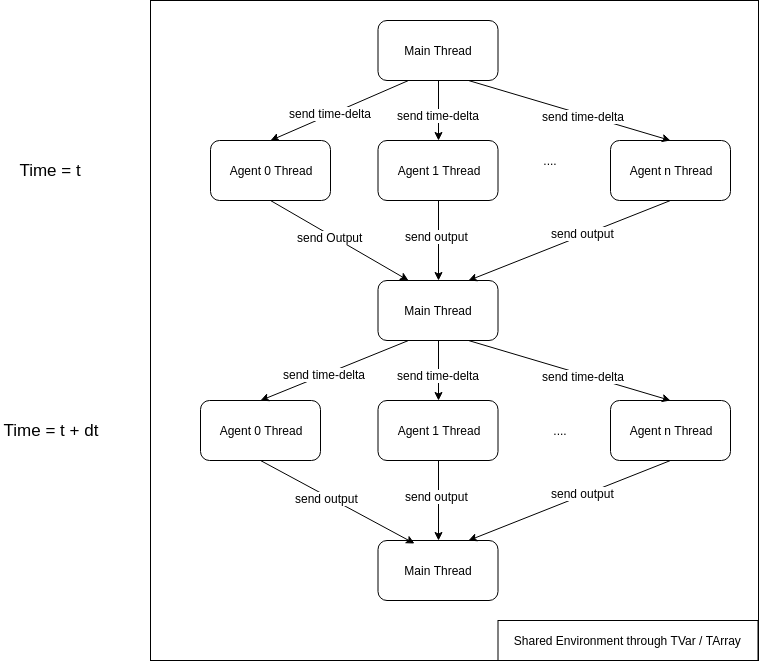
\includegraphics[width=0.7\textwidth, angle=0]{./fig/concurrentabs/stm_abs.png}
	\caption[Diagram of the parallel time-driven lock-step approach]{Diagram of the parallel time-driven lock-step approach.}
	\label{fig:stm_abs_structure}
\end{figure}

\subsection{Adding STM to agents}
We briefly discuss how to add STM to agents on a technical level and also show how to run them within their own threads. We use the SIR implementation as example - applying it to the Sugarscape implementation works exactly the same way and is left as a trivial exercise to the reader.

The first step is to simply add the \texttt{STM} Monad as the innermost level to the already the existing Transformer stack. Further, the environment is now passed as a transactional data primitive to the agent at \textit{construction time}. Thus, the agent does not receive the \texttt{SIREnv} as input any more but receives it through currying when constructing its initial \texttt{MSF}. Further, the agent modifies the \texttt{SIREnv} directly through the \texttt{TVar}, as demonstrated in the case of the infected agent.

\begin{HaskellCode}
-- Make Rand a transformer to be able to add STM as innermost monad
type SIRMonad g = RandT g STM
-- Input to agent is now an empty tuple instead of the Environment
type SIRAgent g = SF (SIRMonad g) () SIRState

-- The MSF construction function takes now the TVar with the environment.
sirAgent :: RandomGen g => TVar SIREnv -> Disc2dCoord -> SIRState -> SIRAgent g

-- The infected agent behaviour is nearly the same except that
-- the agent modifies the environment through the TVar
infected :: RandomGen g => SF (SIRMonad g) () (SIRState, Event ())
infected = proc _ -> do
  recovered <- occasionally illnessDuration () -< ()
  if isEvent recovered
    then (do
      -- update the environment through the TVar
      arrM_ (lift $ lift $ modifyTVar env (changeCell coord Recovered)) -< ()
      returnA -< (Recovered, Event ()))
    else returnA -< (Infected, NoEvent)
\end{HaskellCode}

The agent thread is straightforward. It takes \texttt{MVar} synchronisation primitives to synchronise with the main thread and simply runs the agent behaviour each time it receives the next \textit{DTime}:

\begin{HaskellCode}
agentThread :: RandomGen g 
            => Int             -- ^ Number of steps to compute
            -> SIRAgent g      -- ^ Agent behaviour MSF
            -> g               -- ^ Random-number generator of the agent
            -> MVar SIRState   -- ^ Synchronisation back to main thread
            -> MVar DTime      -- ^ Receiving DTime for next step
            -> IO ()
agentThread 0 _ _ _ _ = return () -- all steps computed, terminate thread
agentThread n sf rng retVar dtVar = do
  -- wait for dt to compute current step
  dt <- takeMVar dtVar

  -- compute output of current step
  let sfReader = unMSF sf ()
      sfRand   = runReaderT sfReader dt
      sfSTM    = runRandT sfRand rng
  -- run the STM action atomically within IO
  ((ret, sf'), rng') <- atomically sfSTM 

  -- post result to main thread
  putMVar retVar ret
  
  -- tail recursion to next step 
  agentThread (n - 1) sf' rng' retVar dtVar
\end{HaskellCode}

Computing a simulation step is now trivial within the main thread. All agent threads \texttt{MVars} are signalled to unblock followed by an immediate block on the \texttt{MVars} into which the agent threads post back their result. The state of the current step is then extracted from the environment, which is stored within the \texttt{TVar} which the agent threads have updated.

\begin{HaskellCode}
simulationStep :: TVar SIREnv     -- ^ environment 
               -> [MVar DTime]    -- ^ sync dt to threads
               -> [MVar SIRState] -- ^ sync output from threads
               -> DTime           -- ^ time delta
               -> IO SIREnv
simulationStep env dtVars retVars dt = do
  -- tell all threads to continue with the corresponding DTime
  mapM_ (`putMVar` dt) dtVars
  -- wait for results but ignore them, SIREnv contains all states
  mapM_ takeMVar retVars
  -- return state of environment when step has finished
  readTVarIO env
\end{HaskellCode}

The difference to an implementation which uses \texttt{IO} are minor but far reaching. Instead of using \texttt{STM} as innermost Monad, we use \texttt{IO}, thus running the whole agent behaviour within the \texttt{IO} Monad. Instead of receiving the environment through a \texttt{TVar}, the agent receives it through an \texttt{IORef}. It also receives an \texttt{MVar} which is the synchronisation primitive to synchronise the access to the environment in the \texttt{IORef} amongst all agents. Agents grab and release the synchronisation lock of the \texttt{MVar} when they enter and leave a critical section in which they operate on the environment stored in the \texttt{IORef}.

\section{Case Study I: SIR}
\label{sec:concurrent_sir}
Our first case study is the SIR model as introduced in Chapter \ref{sec:sir_model}. The aim of this case study is to investigate the potential speed up a concurrent \textit{STM} implementation gains over a sequential one under varying number of CPU cores and agents. The behaviour of the agents is quite simple and the interactions are happening indirectly through the environment, where reads from the environment outnumber the writes to it by far. Further, a comparison to a lock-based implementation with the \textit{IO} Monad is done to understand that \textit{STM} is also able to outperform traditional concurrency, \textit{in a pure functional ABS setting} while still retaining its greater static guarantees than \textit{IO} \footnote{The code of all three implementations is available at \url{https://github.com/thalerjonathan/phd/tree/master/public/stmabs/code/SIR}}.

\begin{enumerate}
	\item Sequential - this is the original implementation as discussed in Chapter \ref{sec:adding_env}, where the discrete 2D environment is shared amongst all agents as read-only data and the agents are executed sequentially within the main thread without any concurrency.
	\item STM - this is the same implementation as the \textit{Sequential} one but agents run now in the \textit{STM} Monad and have access to the discrete 2D environment through a transactional variable \textit{TVar}. This means that the agents now communicate indirectly by reads and writes through the \textit{TVar}.
	\item Lock-Based - this follows the \textit{STM} implementation, with the agents running in \textit{IO}. They share the discrete 2D environment using an \textit{IORef} and have access to an \textit{MVar} lock to synchronise access to it.
\end{enumerate}

Each experiment was run until $t = 100$ and stepped using $\Delta t = 0.1$. For each experiment we conducted 8 runs on our machine (see Table \ref{tab:machine_specs}) under no additional work-load and report the mean. %Further, we checked the visual outputs and the dynamics and they look qualitatively the same as the reference \textit{Sequential}. We could have used more rigour and properly validated the implementations against the formal specification using tests as we do in Chapter Property-based testing but we leave this for further res.
In the experiments we varied the number of agents (grid size) as well as the number of cores when running concurrently - the numbers are always indicated clearly.

\begin{table}
	\centering
	\begin{tabular}{ c || c }
		OS & Fedora 28, 64-bit \\ \hline
		RAM & 16 GByte \\ \hline
		CPU & Intel i5-4670K @ 3.4GHz \\ \hline
		HD & 250Gbyte SSD \\ \hline
		Haskell & GHC 8.2.2
	\end{tabular}
	
	\caption{Machine and Software specs for all experiments}
	\label{tab:machine_specs}
\end{table}

\subsection{Constant Grid Size, Varying Cores}
In this experiment we held the grid size constant to 51 x 51 (2,601 agents) and varied the cores. The results are reported in Table \ref{tab:constgrid_varyingcores}.

\begin{table}
	\centering
	\begin{tabular}{cc|c}
		\multicolumn{1}{ c||  }{\multirow{2}{*}{} } &
		\multicolumn{1}{ |c| }{Cores} & Duration      \\ \hline \hline 
		
		\multicolumn{1}{ c||  }{\multirow{1}{*}{Sequential} } &
		\multicolumn{1}{ |c| }{1} & 72.5      \\ \hline \hline 
		
		\multicolumn{1}{ c||  }{\multirow{4}{*}{Lock-Based} } &
		\multicolumn{1}{ |c| }{1} & 60.6       \\ \cline{2-3}
		\multicolumn{1}{ c||  }{}                       &
		\multicolumn{1}{ |c| }{2} & 42.8    \\ \cline{2-3}
		\multicolumn{1}{ c||  }{}                       &
		\multicolumn{1}{ |c| }{3} & 38.6    \\ \cline{2-3}
		\multicolumn{1}{ c||  }{}                       &
		\multicolumn{1}{ |c| }{4} & 41.6    \\ \hline \hline 
		
		\multicolumn{1}{ c||  }{\multirow{4}{*}{STM} } &
		\multicolumn{1}{ |c| }{1} & 53.2       \\ \cline{2-3}
		\multicolumn{1}{ c||  }{}                       &
		\multicolumn{1}{ |c| }{2} & 27.8    \\ \cline{2-3}
		\multicolumn{1}{ c||  }{}                       &
		\multicolumn{1}{ |c| }{3} & 21.8    \\ \cline{2-3}
		\multicolumn{1}{ c||  }{}                       &
		\multicolumn{1}{ |c| }{4} & \textbf{20.8}    \\ \hline \hline 
	\end{tabular}
  	
  	\caption{Experiments on 51x51 (2,601 agents) grid with varying number of cores. Timings in seconds (lower is better).}
	\label{tab:constgrid_varyingcores}
\end{table}

The \textit{STM} implementation running on 4 cores shows a speed up factor of 3.6 over \textit{Sequential}, which is a quite impressive number when considering that we can achieve at most a factor of 4 when running on 4 cores. It seems that \textit{STM} allow us to push the practical limit very close to the theoretical one, whereas the \textit{Lock-Based} approach just arrives at a factor of 1.74 on 4 cores.

Comparing the performance and scaling to multiple cores shows that the \textit{STM} implementation significantly outperforms the \textit{Lock-Based} one and scales better to multiple cores. The \textit{Lock-Based} implementation performs best with 3 cores and shows slightly worse performance on 4 cores as can be seen in Figure \ref{fig:core_duration_stm_io}. This is no surprise because the more cores are running at the same time, the more contention for the lock, thus the more likely synchronisation happening, resulting in higher potential for reduced performance. This is not an issue in \textit{STM} because no locks are taken in advance. 

\begin{figure}
	\centering
	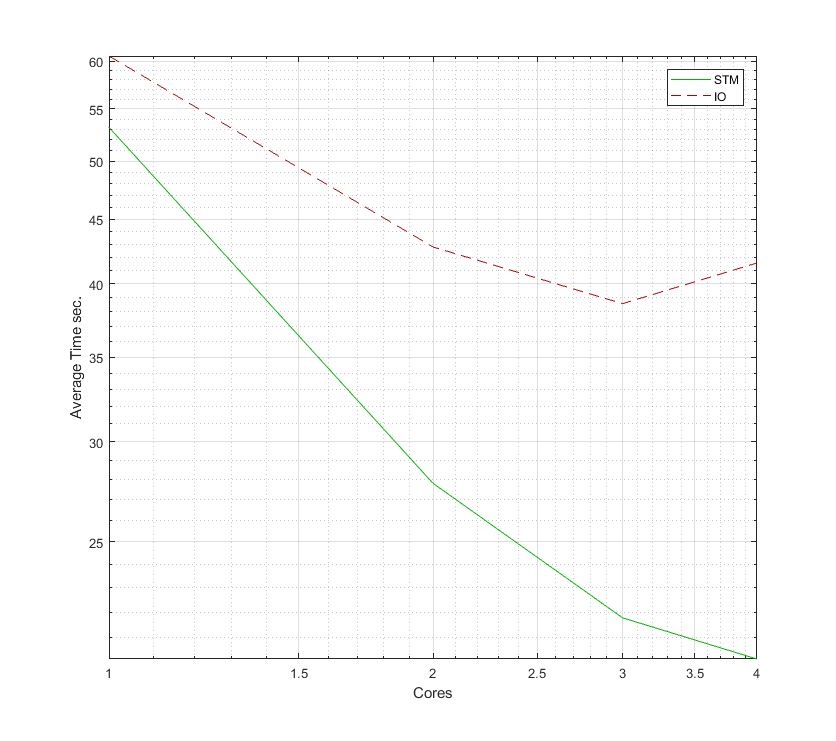
\includegraphics[width=0.8\textwidth, angle=0]{./fig/concurrentabs/sir/core_duration_stm_io.png}
	\caption{Comparison of performance and scaling on multiple cores of STM and Lock-Based. Note that the Lock-Based implementation seems to perform slightly worse on 4 than on 3 cores probably due to lock-contention.}
	\label{fig:core_duration_stm_io}
\end{figure}

\subsection{Varying Grid Size, Constant Cores}
In this experiment we varied the grid size and used always 4 cores. The results are reported in Table \ref{tab:varyinggrid_constcores} and plotted in Figure \ref{fig:varyinggrid_constcores}.

\begin{table}
	\centering
  	\begin{tabular}{ c || c | c | c }
        Grid-Size          & STM              & Lock-Based   & Ratio \\ \hline \hline 
   		51 x 51 (2,601)    & \textbf{20.2}    & 41.9         & 2.1 \\ \hline
   		101 x 101 (10,201) & \textbf{74.5}    & 170.5        & 2.3 \\ \hline
   		151 x 151 (22,801) & \textbf{168.5}   & 376.9        & 2.2 \\ \hline
   		201 x 201 (40,401) & \textbf{302.4}   & 672.0        & 2.2 \\ \hline
   		251 x 251 (63,001) & \textbf{495.7}   & 1,027.3      & 2.1 \\ \hline \hline
  	\end{tabular}

  	\caption{Performance on varying grid sizes. Timings in seconds (lower is better). Ratio compares STM to Lock-Based.}
	\label{tab:varyinggrid_constcores}
\end{table}

It is clear that the \textit{STM} implementation outperforms the \textit{Lock-Based} implementation by a substantial factor.

\begin{figure}
	\centering
	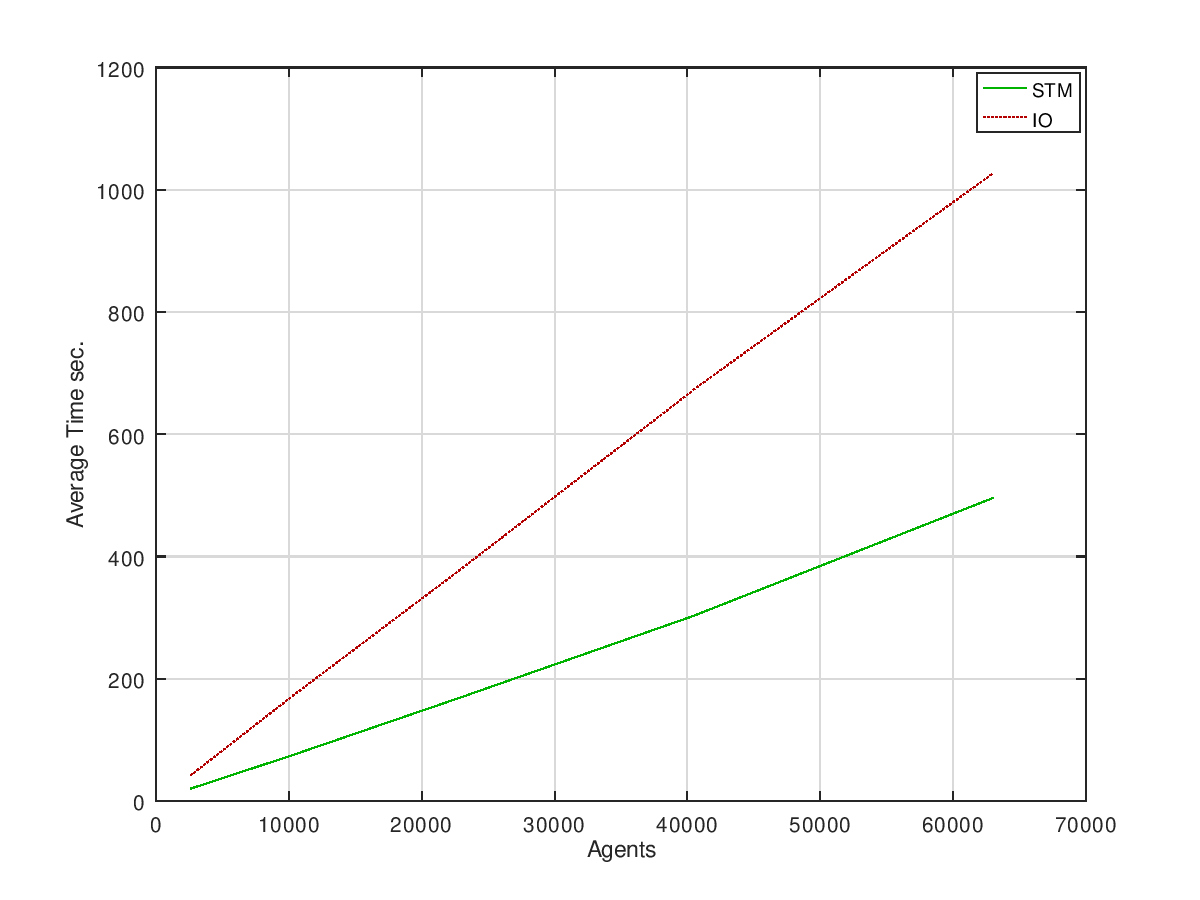
\includegraphics[width=1\textwidth, angle=0]{./fig/concurrentabs/sir/stm_io_varyinggrid_performance.png}
	\caption{Performance on varying grid sizes.}
	\label{fig:varyinggrid_constcores}
\end{figure}

\subsection{Retries}
Of very much interest when using STM is the retry-ratio, which obviously depends highly on the read-write patterns of the respective model. We used the \textit{stm-stats} library to record statistics of commits, retries and the ratio. The results are reported in Table \ref{tab:retries_stm}.

\begin{table}
	\centering
  	\begin{tabular}{ c || c | c | c }
        Grid-Size 		   & Commits    & Retries & Ratio \\ \hline \hline 
   		51 x 51 (2,601)    & 2,601,000  & 1306.5  & 0.0 \\ \hline
   		101 x 101 (10,201) & 10,201,000 & 3712.5  & 0.0 \\ \hline
   		151 x 151 (22,801) & 22,801,000 & 8189.5  & 0.0 \\ \hline
   		201 x 201 (40,401) & 40,401,000 & 13285.0 & 0.0 \\ \hline 
   		251 x 251 (63,001) & 63,001,000 & 21217.0 & 0.0 \\ \hline \hline
  	\end{tabular}
  	
  	\caption{Retry ratios on varying grid sizes on 4 cores.}
	\label{tab:retries_stm}
\end{table}

Independent of the number of agents we always have a retry-ratio of 0.0. This indicates that this model is \textit{very} well suited to STM, which is also directly reflected in the much better performance over the \textit{Lock-Based} implementation. Obviously this ratio stems from the fact that in our implementation we have \textit{very} few writes, which happen only in case when an agent changes from Susceptible to Infected or from Infected to Recovered. On the other hand, there are a very large number of reads due to indirect agent interaction. For \textit{STM} this is no problem because no lock is taken but the \textit{Lock-Based} approach is forced to conservatively take the lock to ensure mutual exclusive access to the critical section across all agents.

\subsection{Going Large-Scale}
To test how far we can scale up the number of cores in both the \textit{Lock-Based} and \textit{STM} cases, we ran two experiments, 51x51 and 251x251, on Amazon EC2 instances with a larger number of cores than our local machinery, starting with 16 and 32 to see if we are running into decreasing returns. The results are reported in Table \ref{tab:sir_varying_cores_amazon}.

\begin{table}
	\centering
  	\begin{tabular}{cc|c|c}
		\multicolumn{1}{ c||  }{\multirow{2}{*}{} } &
		\multicolumn{1}{ |c| }{Cores} & 51x51    & 251x251       \\ \hline \hline 
		
		\multicolumn{1}{ c||  }{\multirow{2}{*}{Lock-Based} } &
		\multicolumn{1}{ |c| }{16} & 72.5    & 1830.5       \\ \cline{2-4}
		\multicolumn{1}{ c||  }{}                       &
		\multicolumn{1}{ |c| }{32} & 73.1    & 1882.2      \\ \hline \hline 
		
		\multicolumn{1}{ c||  }{\multirow{2}{*}{STM} } &
		\multicolumn{1}{ |c| }{16} & \textbf{8.6}     & \textbf{237.0}       \\ \cline{2-4}
		\multicolumn{1}{ c||  }{}                       &
		\multicolumn{1}{ |c| }{32} & 12.0    & 248.7      \\ \hline \hline 
	\end{tabular}

  	\caption{Performance on varying cores on Amazon S2 Services. Timings in seconds (lower is better).}
	\label{tab:sir_varying_cores_amazon}
\end{table}

As expected, the \textit{Lock-Based} approach doesn't scale up to many cores because each additional core brings more contention to the lock, resulting in an even more decreased performance, even worse than the \textit{Sequential} implementation. This is particularly obvious in the 251x251 experiment because of the much larger number of concurrent agents. The \textit{STM} approach returns better performance on 16 cores but fails to scale further up to 32 where the performance drops below the one with 16 cores. In both STM cases we measured a retry-ratio of 0, thus we assume that with 32 cores we become limited by the overhead of STM transactions \cite{perfumo_limits_2008} because the workload of an STM action in our SIR implementation is quite small.

Compared to the \textit{Sequential} implementation, \textit{STM} reaches a speed up factor of 8.4 on 16 cores, which is still impressive but is much further away from the theoretical limit than in the case of only 4 cores -  a further indication that this model in particular and our approach in general does not scale up arbitrarily.

% NOTE: 0 retries in both cases means that the STM transactions themselves are becoming the bottleneck. this makes sens because the STM trasnactions in our SIR implementation are very small (especially recovered and infected agent) and could therefore really cause substantial overhead as pointed out by \cite{perfumo_limits_2008}
%16 cores 251x251: 0.0 retry-ratio
%32 cores 251x251: 0.0 retry ratio
%
%16 cores 51x51: 0.0 retry-ratio
%32 cores 51x51: 0.0 retry ratio

\subsection{Discussion}
The timing measurements speak a clear language: running in \textit{STM} and sharing state using a transactional variable \textit{TVar} is much more time-efficient than both the \textit{Sequential} and \textit{Lock-Based} approach. On 4 cores \textit{STM} achieves a speed up factor of 3.6, nearly reaching the theoretical limit.
Obviously both \textit{STM} and \textit{Lock-Based} sacrifices determinism: repeated runs might not lead to same dynamics despite same initial conditions. Still, by sticking to \textit{STM}, we get the guarantee that the source of this non-determinism is concurrency within the \textit{STM} monad but \textit{nothing else}. This we can not guarantee in the case of the \textit{Lock-Based} approach as all bets are off when running within \textit{IO}. The fact to have \textit{both} the better performance \textit{and} the stronger static guarantees in the \textit{STM} approach makes it \textit{very} compelling.

\section{Case Study II: Sugarscape}
\label{sec:sugarscape_concurrent}
The second case study is the Sugarscape model as introduced in Chapter \ref{sec:sugarscape}. In this case study we look into the potential performance improvement in a model with much more complex agent behaviour and dramatically increased writes on the shared environment.

We implemented the \textit{Carrying Capacity} (p. 30) section of Chapter II of the Sugarscape book \cite{epstein_growing_1996}. In each step agents search (move) to the cell with the most sugar they see within their vision, harvest all of it from the environment and consume sugar because of their metabolism. Sugar regrows in the environment over time. Only one agent can occupy a cell at a time. Agents don't age and cannot die from age. If agents run out of sugar due to their metabolism, they die from starvation and are removed from the simulation. The authors report that the initial number of agents quickly drops and stabilises around a level depending on the model parameters. This is in accordance with our results as we show in Chapter \ref{ch:property} and guarantees that we don't run out of agents. The model parameters are as follows:

\begin{itemize}
	\item Sugar Endowment: each agent has an initial sugar endowment randomly uniform distributed between 5 and 25 units;
	\item Sugar Metabolism: each agent has a sugar metabolism randomly uniform distributed between 1 and 5;
	\item Agent Vision: each agent has a vision randomly uniform distributed between 1 and 6, same for each of the 4 directions (N, W, S, E);
	\item Sugar Growback: sugar grows back by 1.0 unit per step until the maximum capacity of a cell is reached;
	\item Agent Number: initially 500 agents;
	\item Environment Size: 50 x 50 cells with toroid boundaries which wrap around in both x and y dimension.
\end{itemize}

Note that in this implementation (as in the full Chapter II of the book), no direct and no synchronous agent-interactions as we implemented them in Chapter \ref{sec:eventdriven_implementation} are happening. As in the SIR example, all agents interact with each other indirectly through the shared environment. This allows us to regard the implementation as a time-driven, parallel one wherein each step agents act conceptually at the same time.

We compare four different implementations \footnote{The code is freely available at \url{https://github.com/thalerjonathan/phd/tree/master/public/stmabs/code/SugarScape}}:

\begin{enumerate}
	\item Sequential - All agents are run after another (including the environment) and the environment is shared amongst the agents using a \textit{StateT} transformer.
	\item Lock-Based - All agents are run concurrently in the \textit{IO} monad and the environment is shared between the agents, using an \textit{IORef} with the access synchronised through an \textit{MVar} lock.
	\item STM TVar - All agents are run concurrently in the \textit{STM} monad and the environment is shared using a \textit{TVar} between the agents.
	\item STM TArray - All agents are run concurrently in the \textit{STM} monad and the environment is shared using a \textit{TArray} between the agents. 
\end{enumerate}

We follow \cite{lysenko_framework_2008} and measure the average number of steps per second of the simulation over 60 seconds. For each experiment we conducted 8 runs on our machine (see Table \ref{tab:machine_specs}) under no additional work-load and report the average. In the experiments we varied the number of cores when running concurrently - the numbers are always indicated clearly.

%\paragraph{Output} Note that we omit the graphical rendering in the functional approach because it is a serious bottleneck taking up substantial amount of the simulation time. Although visual output is often important in ABS, it is not what we are interested here thus we completely omit it and only output the number of agents in the simulation at each step piped into a file, thus omitting slow output to the console \footnote{Note that we need to produce \textit{some} output because of Haskells laziness - if we wouldn't output anything from the simulation then the expressions would actually never be fully evaluated thus resulting in high number of steps per second but which obviously don't really reflect the true computations done.}.

\paragraph{Ordering} The model specification requires to shuffle agents before every step (Footnote 12 on page 26 \cite{epstein_growing_1996}). In the \textit{Sequential} approach we do this explicitly but in the \textit{Lock-Based} and both \textit{STM} approaches we assume this to happen automatically due to race-conditions in concurrency, thus we arrive at an effectively shuffled processing of agents: we implicitly assume that the order of the agents is \textit{effectively} random in every step. The important difference between the two approaches is that in the \textit{Sequential} approach we have full control over this randomness but in the \textit{STM} not - also this means that repeated runs with the same initial conditions might lead to slightly different results. 
This decision leaves the execution order of the agents ultimately to Haskell's Runtime System and the underlying OS. We are aware that by doing this, we make assumptions that the threads run uniformly distributed (fair) but such assumptions should not be made in concurrent programming. As a result we can expect this fact to produces non-uniform distributions of agent runs but we assumed that for this model this does not has a significance influence - in case of doubt, we could resort to shuffling the agents before running them in every step. We agree that this very problem would deserve in-depth research on its own, where also the influence of non-deterministic ordering on the correctness and results of ABS has to be analysed. This is not the main interest of this section though and we leave it for further research as it is completely beyond the focus of this thesis.

%Note that in the concurrent implementations we have two options for running the environment: either asynchronously as a concurrent agent at the same time with the population agents or synchronously after all agents have run. We must be careful though as running the environment as a concurrent agent can be seen as conceptually wrong because the time when the regrowth of the sugar happens is now completely random. In this case it could happen that sugar regrows in the very first transaction or in the very last, different in each step, which can be seen as a violation of the model specifications. Thus we do not run the environment concurrently with the agents but synchronously after all agents have run.

\subsection{Constant Agent Size}
In a first approach we compare the performance of all implementations on varying numbers of cores. The results are reported in Table \ref{tab:varying_cores} and plotted in Figure \ref{fig:varying_cores}. 

\begin{table}
	\centering
	\begin{tabular}{cc|c|c}
		\multicolumn{1}{ c||  }{\multirow{2}{*}{} } &
		\multicolumn{1}{ |c| }{Cores} & Steps & Retries      \\ \hline \hline 
		
		\multicolumn{1}{ c||  }{\multirow{1}{*}{Sequential} } &
		\multicolumn{1}{ |c| }{1} & 39.4 & N/A     \\ \hline \hline 
		
		\multicolumn{1}{ c||  }{\multirow{4}{*}{Lock-Based} } &
		\multicolumn{1}{ |c| }{1} & 43.0 & N/A       \\ \cline{2-4}
		\multicolumn{1}{ c||  }{}                       &
		\multicolumn{1}{ |c| }{2} & 51.8 & N/A   \\ \cline{2-4}
		\multicolumn{1}{ c||  }{}                       &
		\multicolumn{1}{ |c| }{3} & 57.4 & N/A   \\ \cline{2-4}
		\multicolumn{1}{ c||  }{}                       &
		\multicolumn{1}{ |c| }{4} & 58.1 & N/A   \\ \hline \hline 
		
		\multicolumn{1}{ c||  }{\multirow{4}{*}{STM \textit{TVar}} } &
		\multicolumn{1}{ |c| }{1} & \textbf{47.3} & 0.0       \\ \cline{2-4}
		\multicolumn{1}{ c||  }{}                       &
		\multicolumn{1}{ |c| }{2} & 53.5 & 1.1    \\ \cline{2-4}
		\multicolumn{1}{ c||  }{}                       &
		\multicolumn{1}{ |c| }{3} & 57.1 & 2.2    \\ \cline{2-4}
		\multicolumn{1}{ c||  }{}                       &
		\multicolumn{1}{ |c| }{4} & 53.0 & 3.2   \\ \hline \hline 
		
		\multicolumn{1}{ c||  }{\multirow{4}{*}{STM \textit{TArray}} } &
		\multicolumn{1}{ |c| }{1} & 45.4 & 0.0       \\ \cline{2-4}
		\multicolumn{1}{ c||  }{}                       &
		\multicolumn{1}{ |c| }{2} & \textbf{65.3} & 0.02   \\ \cline{2-4}
		\multicolumn{1}{ c||  }{}                       &
		\multicolumn{1}{ |c| }{3} & \textbf{75.7} & 0.04    \\ \cline{2-4}
		\multicolumn{1}{ c||  }{}                       &
		\multicolumn{1}{ |c| }{4} & \textbf{84.4} & 0.05   \\ \hline \hline 
	\end{tabular}  	
  	
  	\caption{Steps per second and retries on 50x50 grid with 500 initial agents on varying cores.}
	\label{tab:varying_cores}
\end{table}

\begin{figure}
	\centering
	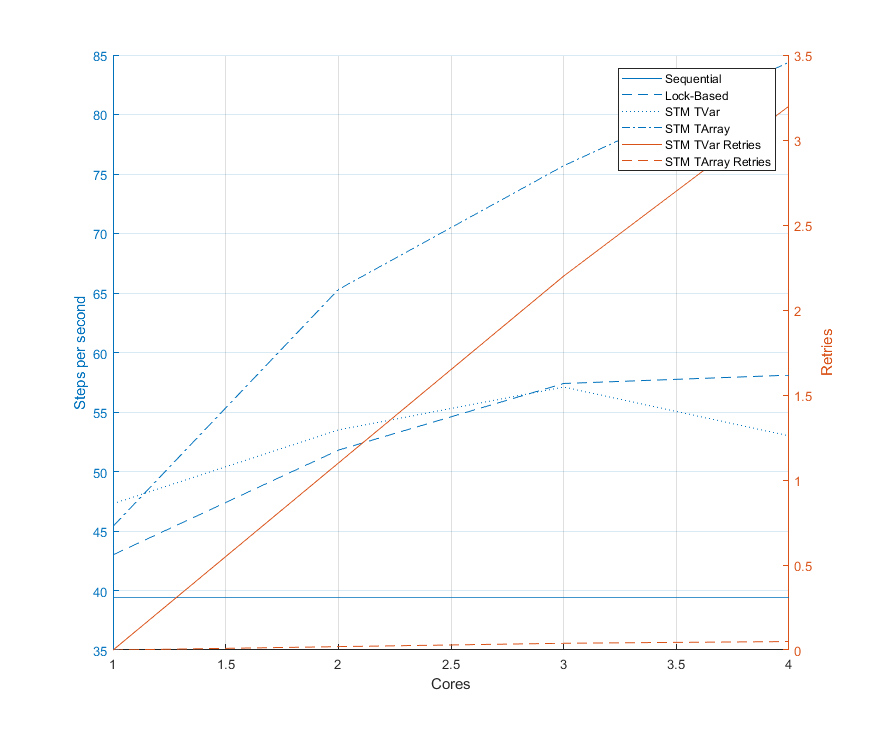
\includegraphics[width=0.7\textwidth, angle=0]{./fig/concurrentabs/sugarscape/varying_cores.png}
	\caption{Steps per second and retries on 50x50 grid and 500 initial agents on varying cores.}
	\label{fig:varying_cores}
\end{figure}

As expected, the \textit{Sequential} implementation is the slowest, followed by the \textit{Lock-Based} and \textit{TVar} approach whereas \textit{TArray} is the best performing one.

We clearly see that using a \textit{TVar} to share the environment is a very inefficient choice in this model: \textit{every} write to a cell leads to a retry independent whether the reading agent reads that changed cell or not, because the data-structure can not distinguish between individual cells. By using a \textit{TArray} we can avoid the situation where a write to a cell in a far distant location of the environment will lead to a retry of an agent which never even touched that cell. Also the \textit{TArray} seems to scale up by 10 steps per second for every core added. It will be interesting to see how far this could go with the Amazon experiment, as we seem not to hit a limit with 4 cores yet.

The inefficiency of \textit{TVar} is also reflected in the nearly similar performance of the \textit{Lock-Based} implementation which even outperforms it on 4 cores. This is due to very similar approaches because both operate on the whole environment instead of only the cells as \textit{TArray} does. This seems to be a bottleneck in \textit{TVar} reaching the best performance on 3 cores, which then drops on 4 cores due to an increasing retries ratio. The \textit{Lock-Based} approach seems to reduce its returns on increased number of cores hitting a limit at 4 cores as well.

\subsection{Scaling up Agents}
So far we kept the initial number of agents at 500, which due to the model specification, quickly drops and stabilises around 200 due to the carrying capacity of the environment as described in the book \cite{epstein_growing_1996} section \textit{Carrying Capacity} (p. 30).

We now want to measure the performance of our approaches under increased number of agents. For this we slightly change the implementation: always when an agent dies it spawns a new one which is inspired by the ageing and birthing feature of Chapter III in the book \cite{epstein_growing_1996}. This ensures that we keep the number of agents roughly constant (still fluctuates but doesn't drop to low levels) over the whole duration. This ensures a constant load of concurrent agents interacting with each other and demonstrates also the ability to terminate and create concurrent agents (threads) dynamically during the simulation.

Except for the \textit{Sequential} approach we ran all experiments with 4 cores (TVar with 3 as well). We looked into the performance of 500, 1,000, 1,500, 2,000 and 2,500 (maximum possible capacity of the 50x50 environment). The results are reported in Table \ref{tab:state_results_agentsscale_time} and plotted in Figure \ref{fig:state_results_agentsscale_time}.

\begin{table}
	\centering
  	\begin{tabular}{ c || c | c | c | c | c }
        Agents  & Sequential & Lock-Based & TVar (3 cores) & TVar (4 cores) & TArray  \\ \hline \hline 
    	    500     & 14.4       & 20.2		  &	20.1           & 18.5       	& \textbf{71.9}    \\ \hline
   		1,000   & 6.8        & 10.8 	      & 10.4           & 9.5         & \textbf{54.8}    \\ \hline
   		1,500   & 4.7        & 8.1 		  & 7.9            & 7.3			& \textbf{44.1}    \\ \hline
   		2,000   & 4.4        & 7.6 		  & 7.4            & 6.7    		& \textbf{37.0}    \\ \hline 
   		2,500   & 5.3        & 5.4 		  & 9.2            & 8.9			& \textbf{33.3}    \\ \hline \hline
   	\end{tabular}
  	
  	\caption{Steps per second on 50x50 grid with varying number of agents with 4 (and 3) cores except Sequential (1 core).}
	\label{tab:state_results_agentsscale_time}
\end{table}

\begin{figure}
	\centering
	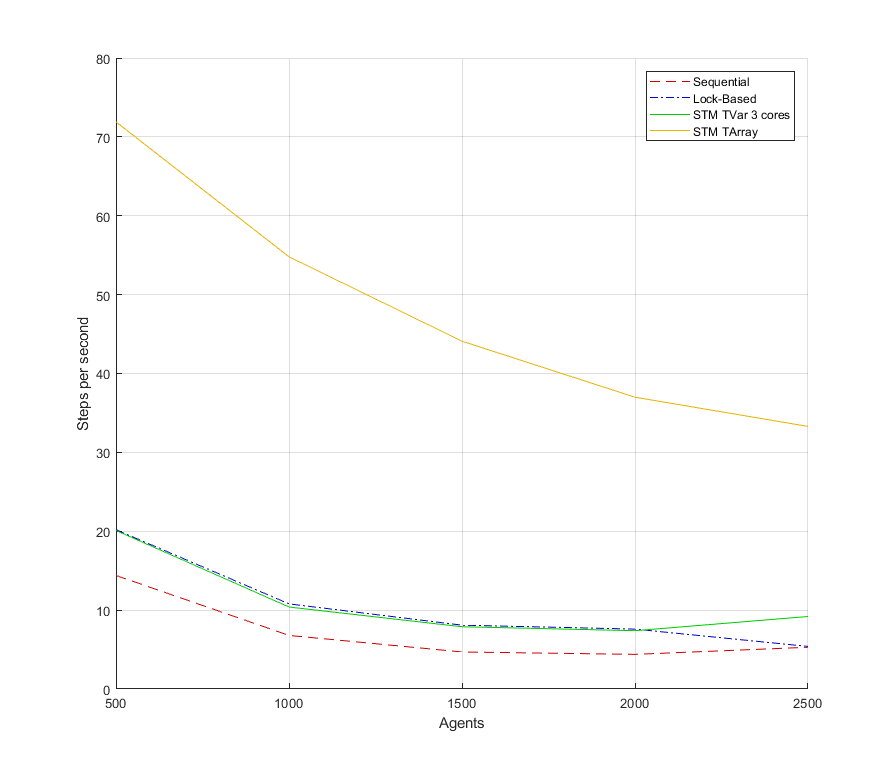
\includegraphics[width=1.0\textwidth, angle=0]{./fig/concurrentabs/sugarscape/varying_agents.png}
	\caption{Steps per second on 50x50 grid and varying number of agents with 4 (and 3) cores except Sequential (1 core).}
	\label{fig:state_results_agentsscale_time}
\end{figure}

As expected, the \textit{TArray} implementation outperforms all others substantially. Also as expected, the \textit{TVar} implementation on 3 cores is faster than on 4 cores as well when scaling up to more agents. The \textit{Lock-Based} approach performs about the same as the \textit{TVar} on 3 cores because of the very similar approaches: both access the \textit{whole} environment. Still the \textit{TVar} approach uses one core less to arrive at the same performance, thus strictly speaking outperforming the \textit{Lock-Based} implementation.

What seems to be very surprising is that in the \textit{Sequential} and \textit{TVar} cases the performance with 2,500 agents is \textit{better} than the one with 2,000 agents. The reason for this is that in the case of 2,500 agents, an agent can't move anywhere because all cells are already occupied. In this case the agent won't rank the cells in order of their pay-off (max sugar) to move to but just stays where it is. We hypothesize that due to Haskells laziness the agents actually never look at the content of the cells in this case but only the number which means that the cells themselves are never evaluated which further increases performance. This leads to the better performance in case of \textit{Sequential} and \textit{TVar} because both exploit laziness.
In the case of the \textit{Lock-Based} approach we still arrive at a lower performance because the limiting factor are the unconditional locks. In the case of the \textit{TArray} approach we also arrive at a lower performance because it seems that STM perform reads on the neighbouring cells which are not subject to lazy evaluation. In Haskell it is notoriously difficult to reason about efficiency (see Chapter \ref{ch:drawbacks} for a short discussion on drawbacks) and this behaviour of improved performance due to Haskells lazyness is no exception. We leave an in-depth investigation for further research as it is beyond the focus of this chapter.

We also measured the average retries both for \textit{TVar} and \textit{TArray} under 2,500 agents where the \textit{TArray} approach shows best scaling performance with 0.01 retries whereas \textit{TVar} averages at 3.28 retries. Again this can be attributed to the better transactional data-structure which reduces retry-ratio substantially to near-zero levels.

\subsection{Going Large-Scale}
To test how far we can scale up the number of cores in both the \textit{Lock-Based} and \textit{TArray} cases, we ran the two experiments (carrying capacity and rebirthing) on Amazon EC2 instances with increasing number of cores starting with 16 and 32 to see if we run into decreasing returns. The results are reported in Table \ref{tab:sug_varying_cores_amazon}.

\begin{table}
	\centering
%  	\begin{tabular}{ c || c | c | c }
%                   & Cores & Carrying Capacity & Rebirthing  \\ \hline \hline 
%    	Lock-Based & 16    & 53.9              & 4.4         \\ \hline
%    	Lock-Based & 32    & 44.2              & 3.6         \\ \hline \hline 
%   		
%   		STM TArray & 16    & \textbf{116.8} (0.23)      & \textbf{39.5} (0.08) \\ \hline
%   		STM TArray & 32    & 109.8 (0.41)      & 31.3 (0.18) \\ \hline \hline 
%   	\end{tabular}
  	
	\begin{tabular}{cc|c|c}
		\multicolumn{1}{ c||  }{\multirow{2}{*}{} } &
		\multicolumn{1}{ |c| }{Cores} & Carrying Capacity    & Rebirthing       \\ \hline \hline 
		
		\multicolumn{1}{ c||  }{\multirow{2}{*}{Lock-Based} } &
		\multicolumn{1}{ |c| }{16} & 53.9              & 4.4       \\ \cline{2-4}
		\multicolumn{1}{ c||  }{}                       &
		\multicolumn{1}{ |c| }{32} & 44.2              & 3.6      \\ \hline \hline 
		
		\multicolumn{1}{ c||  }{\multirow{2}{*}{STM TArray} } &
		\multicolumn{1}{ |c| }{16} & \textbf{116.8} (0.23)      & \textbf{39.5} (0.08)       \\ \cline{2-4}
		\multicolumn{1}{ c||  }{}                       &
		\multicolumn{1}{ |c| }{32} & \textbf{109.8} (0.41)      & \textbf{31.3} (0.18)      \\ \hline \hline 
	\end{tabular}  	
  	
  	\caption{Steps per second on varying cores on Amazon S2 Services.}
	\label{tab:sug_varying_cores_amazon}
\end{table}

As expected, the \textit{Lock-Based} approach doesn't scale up to many cores because each additional core brings more contention to the lock, resulting in even more decreased performance. This is particularly obvious in the rebirthing experiment because of the much larger number of concurrent agents. The \textit{TArray} approach returns better performance on 16 cores but fails to scale further up to 32 where the performance drops below the one with 16 cores. We indicated the retry-ratio in brackets and see that they roughly double from 16 to 32, which is the reason why performance drops as at this point. 

%the INCREASE in time can only happen due to more retries
%Carrying Capacity 16 core ~ 0.23 retry-ratio
%Carrying Capacity 32 core ~ 0.41 retry-ratio
%
%Rebirthing 16 core ~ 0.08 retry-ratio
%Rebirthing 32 core ~ 0.18 retry-ratio

\subsection{Comparison with other approaches}
The paper \cite{lysenko_framework_2008} reports a performance of 17 steps in RePast, 18 steps in MASON (both non-parallel) and 2,000 steps per second on a GPU on a 128x128 grid. Although our \textit{Sequential} implementation, which runs non-parallel as well, outperforms the RePast and MASON implementations of \cite{lysenko_framework_2008}, one must be very well aware that these results were generated in 2008, on current hardware of that time.

%When we run the SugarScape example of RePast with the same model parameters as ours on the same machine (see Table \ref{tab:machine_specs}) we arrive at roughly 450 steps per second - a factor of about 3.8 faster than even our STM \textit{TArray} implementation on 16 cores. This might seem quite shocking, even more so because RePast also performs visual output, rendering the SugarScape in every step. When scaling up the agents to 2,500 the RePast version arrives around roughly 95 steps per second which is still faster by a factor of 3 than our 4 core \textit{TArray} implementation. We attribute this substantial performance difference to the inherent performance difference of functional programming to imperative approaches as already outlined in the previous section. 

The very high performance on the GPU does not concern us here as it follows a very different approach than ours. We focus on speeding up implementations on the CPU as directly as possible without locking overhead. When following a GPU approach one needs to map the model to the GPU which is a delicate and non-trivial matter. With our approach we show that speed up with concurrency is very possible without the low-level locking details or the need to map to GPU. Also some features as bilateral trading between agents, where a pair of agents needs to come to a conclusion over multiple synchronous steps, is difficult to implement on a GPU whereas this is easily possible using STM.

Note that we kept the grid-size constant because we implemented the environment as a single agent which works sequentially on the cells to regrow the sugar. Obviously this doesn't really scale up on parallel hardware and experiments which we haven't included here due to lack of space, show that the performance goes down dramatically when we increase the environment to 128x128 with same number of agents which is the result of Amdahl's law where the environment becomes the limiting factor of the simulation. Depending on the underlying data-structure used for the environment we have two options to solve this problem. In the case of the \textit{Sequential} and \textit{TVar} implementation we build on an indexed array, which we can be updated in parallel using the existing data-parallel support in Haskell. In the case of the \textit{TArray} approach we have no option but to run the update of every cell within its own thread. We leave both for further research as it is out of scope of this paper.

\subsection{Discussion}
This case study showed clearly that besides being substantially faster than the \textit{Sequential} implementation, \textit{STM} is also able to perform considerably better than a \textit{Lock-Based} approach even in the case of a model with much higher complexity in agent behaviour and dramatically increased number of writes to the environment.
Further, this case study demonstrated that the selection of the right transactional data-structure is of fundamental importance when using \textit{STM}. Selecting the right transactional data-structure is very model-specific and can lead to dramatically different performance results.
In this case the \textit{TArray} performed best due to many writes but in the SIR case-study a \textit{TVar} showed good enough results due to the very low number of writes. When not carefully selecting the right transactional data-structure which supports fine-grained concurrency, a lock-based implementation might perform as well or even outperform the STM approach as can be seen when using the \textit{TVar}.
Although the \textit{TArray} is the better transactional data-structure overall, it might come with an overhead, performing worse on low number of cores than a \textit{TVar} approach but has the benefit of quickly scaling up to multiple cores. Depending on the transactional data-structure, scaling up to multiple cores hits a limit at some point. In the case of the \textit{TVar} the best performance is reached with 3 cores. With the \textit{TArray} we reached this limit around 16 cores.

Note that the comparison between the \textit{Lock-Based} approach and the \textit{STM TArray} implementation is a bit unfair due to a very different locking structure. A more suitable comparison would have been to use an indexed Array with a tuple of (MVar, IORef) in each cell to support fine-grained locking on cell-level. This would be a more just comparison to the \textit{STM Array} where fine-grained transactions happen on the cell-level. We hypothesize that \textit{STM} will still outperform the \textit{IO} approach but to a lesser degree - we leave the proof of this for further research.

%Unfortunately, for this model the performance is nowhere comparable to imperative approaches, which we attribute to the inherent performance difference of functional programming to imperative approaches. With the use of advanced language features we might arrive at much improved performance but we leave this for further research as we focus primarily on the comparison between lock-based and STM approaches.

%we can implement everything except synchronous direct agent-interactions atm: if agent-interaction is one-way e.g. paying back a loan then this is no problem. thus the following parts of the Sugarscape are not possible with our current STM approach: mating, trading and lending  because all 3 require direct agent-to-agent interaction over multiple steps. We leave the problem of developing such an algorithm / implementation for further research.

\section{Discussion}
Although there are similarities to the work of \cite{botta_time_2010} (the use of messages and the problem of when to advance time in models with arbitrary number synchronised agent-interactions), we approach our agents differently. First in our approach an agent is only a single MSF and thus can not be directly queried for its internal state / its id or outgoing messages, instead of taking a list of messages, our agents take a single event/message and can produce an arbitrary number of outgoing messages together with an observable state - note that this would allow to query the agent for its id and its state as well by simply sending a corresponding message to the agents MSF and requiring the agent to implement message handling for it. Also the state of our agents is \textit{completely} localised and there is no means of accessing the state from outside the agent, they are thus "fully encapsulated agents" \cite{botta_time_2010}. Note that the authors of \cite{botta_time_2010} define their agents with a polymorphic agent-state type \textit{s}, which implies that without knowledge of the specific type of \textit{s} there would be no way of accessing the state, rendering it in fact also fully encapsulated. The problem of advancing time in our approach is solved not exactly the same but conceptually it is the same: after sending a tick message to each agent (in random order), we process all agents until they are idle: there are no more enqueued messages / events in the queue.

our eventdriven approach makes heavy use of 2 state monads, thus one might ask what the benefits are, after all we seem to fall back into stateful, imperative style programming. we agree that our approach is just one way of implementing abs in fp but we think we have come a long way thus making our approach quite valuable even if there might be other approaches like shallow EDSLs. on the other hand even our stateful programming is highly restricted to only those 2 local datatypes which makes it much more manageable than unrestricted data mutation

quote carmack (\url{http://www.gamasutra.com/view/news/169296/Indepth_Functional_programming_in_C.php}): the main difficulty as a developer in software programming is to keep track of the states a program can be in and reason about them and their Validity

TODO: report LoC and compare it with other implementations we found on the internet

% PART V: Why 2
\epigraphhead[450]{}
\part{Property-Based testing}
\chapter*{} %Property-Based Testing in pure functional ABS
\label{ch:property}

TODO: don't use resize population and always use normal size to be consistent
TODO: feed random population as random parameter
TODO: use TimeRange and UnitRange consistently everywhere

TODO WORDING: don't use replications in terms of QuickCheck! we test properties with random test-cases

TODO IMPROVE EXPLANATION: more explanations, its too flat, code straight in the face, prepare it gently as it is not directly clear what the intention is. discuss it more generally, otherwise it reads like an advanced technical report and not like a thesis.

TODO: explain more how and why and when we use cover and checkCoverage. Also when using cover we cannot use random model parameters as it changes distributions

TODO: only use cover with/without checkCoverage instead of maxFailPercent

TODO: "Contrary to a lot of misinformation, unit testing in Haskell is quite common and robust. Although generally speaking unit tests tend to be of less importance in Haskell since the type system makes an enormous amount of invalid programs completely inexpressible by construction. Unit tests tend to be written later in the development lifecycle and generally tend to be about the core logic of the program and not the intermediate plumbing." cited from section "Testing" in Stephen Diel What I wish i knew \url{http://dev.stephendiehl.com/hask/#testing}.

When implementing an Agent-Based Simulation (ABS) it is of fundamental importance that the implementation is correct up to some specification and that this specification matches the real world in some way. This process is called verification and validation (V\&V), where \textit{validation} is the process of ensuring that a model or specification is sufficiently accurate for the purpose at hand whereas \textit{verification} is the process of ensuring that the model design has been transformed into a computer model with sufficient accuracy \cite{robinson_simulation:_2014}. In other words, validation determines if we are we building the \textit{right model}, and verification if we are building the \textit{model right} up to some specification \cite{balci_verification_1998}.

% there is no general validity, an approach is TDD: V&V particularly difficult in ABS
One can argue that ABS should require more rigorous programming standards than other computer simulations \cite{polhill_ghost_2005}. Because researchers in ABS look for an emergent behaviour in the dynamics of the simulation, they are always tempted to look for some surprising behaviour and expect something unexpected from their simulation. 
Also, due to ABS' \textit{constructive / exploratory} nature \cite{epstein_chapter_2006, epstein_generative_2012}, there exists some uncertainty about the dynamics the simulation will produce before running it. The authors \cite{ormerod_validation_2006} see the current process of building ABS as a discovery process where models of an ABS often lack an analytical solution in general, which makes verification much harder if there is no such solution. Thus it is often very difficult to judge whether an unexpected outcome can be attributed to the model or has in fact its roots in a subtle programming error \cite{galan_errors_2009}.

In general this implies that it is not possible to prove that a model is valid in general but that the best we can do is to \textit{raise the confidence} in the correctness of the simulation. Therefore, the process of V\&V is not the proof that a model is correct but the \textit{process} of trying to show that the model is \textit{not incorrect}. The more checks one carries out which show that it is not incorrect, the more confidence we can place on the models validity. To tackle such a problem in software, software engineers have developed the concept of test-driven development (TDD).

Test-Driven Development (TDD) was popularised in the early 00s by Kent Beck \cite{beck_test_2002} as a way to a more agile approach to software-engineering, where instead of doing each step (requirements, implementation, testing,...) as separated from each other, all of them are combined in shorter cycles. Put shortly, in TDD tests are written for each feature before actually implementing it, then the feature is fully implemented and the tests for it should pass. This cycle is repeated until the implementation of all requirements has finished. Traditionally TDD relies on so called unit-tests which can be understood as a piece of code which when run isolated, tests some functionality of an implementation. Thus we can say that test-driven development in general and unit testing together with code-coverage in particular, guarantee the correctness of an implementation to some informal degree, which has been proven to be sufficiently enough through years of practice in the software industry all over the world. 

\medskip

The work \cite{collier_test-driven_2013} was the first to discusses how to apply TDD to ABS, using unit testing to verify the correctness of the implementation up to a certain level. They show how to implement unit-tests within the RePast Framework \cite{north_complex_2013} and make the important point that such a software needs to be designed to be sufficiently modular otherwise testing becomes too cumbersome and involves too many parts. The paper \cite{asta_investigation_2014} discusses a similar approach to DES in the AnyLogic software toolkit. 

The paper \cite{onggo_test-driven_2016} proposes Test Driven Simulation Modelling (TDSM) which combines techniques from TDD to simulation modelling. The authors present a case study for maritime search-operations where they employ ABS. They emphasise that simulation modelling is an iterative process, where changes are made to existing parts, making a TDD approach to simulation modelling a good match. They present how to validate their model against analytical solutions from theory using unit-tests by running the whole simulation within a unit-test and then perform a statistical comparison against a formal specification. %This approach will become of importance later on in our SIR and Sugarscape case studies.

The paper \cite{gurcan_generic_2013} gives an in-depth and detailed overview over verification, validation and testing of agent-based models and simulations and proposes a generic framework for it. The authors present a generic UML class model for their framework which they then implement in the two ABS frameworks RePast and MASON. Both of them are implemented in Java and the authors provide a detailed description how their generic testing framework architecture works and how it utilises unit testing with JUnit to run automated tests. To demonstrate their framework they provide also a case study of an agent-base simulation of synaptic connectivity where they provide an in-depth explanation of their levels of test together with code.

\medskip

% the gap
Although it would be interesting to see how we can apply unit testing to our approach, it is straight forward, nothing new and does not constitute unique research. Thus, in this chapter we introduce an additional technique for TDD: \textit{property-based testing}, which can be seen as complementary to unit testing. Property-based testing has its origins \cite{claessen_quickcheck_2000,claessen_testing_2002,runciman_smallcheck_2008} in Haskell, where it was first conceived and implemented. It has been successfully used for testing Haskell code for years and also been proven to be useful in the industry \cite{hughes_quickcheck_2007}. We show and discuss how this technique can be applied to test pure functional ABS implementations. To our best knowledge property-based testing has never been looked at in the context of ABS and this thesis is the first one to do so.

\medskip

The main idea of property-based testing is to express model-specifications and laws directly in code and test them through \textit{automated} and \textit{randomised} test-data generation. Thus one hypothesis of this thesis is that due to ABS \textit{stochastic} and \textit{exploratory / generative / constructive } nature, property-based testing is a natural fit for testing ABS in general and pure functional ABS implementations in particular. It thus should pose a valuable addition to the already existing testing methods in this field, worth exploring. To substantiate and test our hypothesis, we present two case-studies. First, the agent-based SIR model as introduced in Chapter \ref{sec:sir_model}, which is of explanatory nature, where we show how to express formal model-specifications in property-tests. Second, the SugarScape model as introduced in Chapter \ref{sec:sugarscape}, which is of exploratory nature, where we show how to express hypotheses in property-tests and how to property-test agent functionality. Note that we only focus on ABS specific testing in the form of model verification, individual agent behaviour and agent interaction testing. We don't look into obvious applications of QuickCheck like testing boundary-checks of the environment, helper functions of agents,... as although they are used within ABS, there is nothing new in testing them with QuickCheck.
%Again, we emphasise that we see it as an addition to TDD, where it works in combination with unit testing to verify and validate a simulation to increase the confidence in its correctness. % and is a useful tool for expressing regression tests.

\medskip

Note that property-based testing has a close connection to model-checking \cite{mcmillan_symbolic_1993}, where properties of a system are proved in a formal way. The important difference is that the checking happens directly on code and not on the abstract, formal model, thus one can say that it combines model-checking and unit testing, embedding it directly in the software-development and TDD process without an intermediary step. We hypothesise that adding it to the already existing testing methods in the field of ABS is of substantial value as it allows to cover a much wider range of test-cases due to automatic data generation. This can be used in two ways: to verify an implementation against a formal specification and to test hypotheses about an implemented simulation. This puts property-based testing on the same level as agent- and system testing, where not technical implementation details of e.g. agents are checked like in unit-tests but their individual complete behaviour and the system behaviour as a whole.

The work \cite{onggo_test-driven_2016} explicitly mentions the problem of test coverage which would often require to write a large number of tests manually to cover the parameter ranges sufficiently enough - property-based testing addresses exactly this problem by \textit{automating} the test-data generation. Note that this is closely related to data-generators \cite{gurcan_generic_2013}, load generators and random testing \cite{burnstein_practical_2010}. Property-based testing though goes one step further by integrating this into a specification language directly into code, emphasising a declarative approach and pushing the generators behind the scenes, making them transparent and focusing on the specification rather than on the data-generation. 

\section*{Property-Based Testing}
\label{sec:proptesting}

Property-based testing allows to formulate \textit{functional specifications} in code which then a property-based testing library tries to falsify by \textit{automatically} generating test-data, covering as much cases as possible. When a case is found for which the property fails, the library then reduces the test-data to its simplest form for which the test still fails e.g. shrinking a list to a smaller size. It is clear to see that this kind of testing is especially suited to ABS, because we can formulate specifications, meaning we describe \textit{what} to test instead of \textit{how} to test. Also the deductive nature of falsification in property-based testing suits very well the constructive and exploratory nature of ABS. Further, the automatic test-generation can make testing of large scenarios in ABS feasible because it does not require the programmer to specify all test-cases by hand, as is required in e.g. traditional unit tests.

Property-based testing was introduced in \cite{claessen_quickcheck_2000,claessen_testing_2002} where the authors present the QuickCheck library in Haskell, which tries to falsify the specifications by \textit{randomly} sampling the test space. We argue, that the stochastic sampling nature of this approach is particularly well suited to ABS, because it is itself almost always driven by stochastic events and randomness in the agents behaviour, thus this correlation should make it straightforward to map ABS to property-testing.
%The main challenge when using QuickCheck, as will be shown later, is to write \textit{custom} test-data generators for agents and the environment which cover the space sufficiently enough to not miss out on important test-cases.
According to the authors of QuickCheck \textit{"The major limitation is that there is no measurement of test coverage."} \cite{claessen_quickcheck_2000}. Although QuickCheck provides help to report the distribution of test-cases it is not able to measure the coverage of tests in general. This could lead to the case that test-cases which would fail are never tested because of the stochastic nature of QuickCheck. Fortunately, the library provides mechanisms for the developer to measure coverage in specific test-cases where the data and its (expected) distribution is known to the developer. This is a powerful tool for testing randomness in ABS as will be shown in subsequent chapters.

\medskip

As a remedy for the potential coverage problems of QuickCheck, there exists also a deterministic property-testing library called SmallCheck \cite{runciman_smallcheck_2008}, which instead of randomly sampling the test-space, enumerates test-cases exhaustively up to some depth. It is based on two observations, derived from model-checking, that (1) \textit{"If a program fails to meet its specification in some cases, it almost always fails in some simple case"} and (2) \textit{"If a program does not fail in any simple case, it hardly ever fails in any case} \cite{runciman_smallcheck_2008}. This non-stochastic approach to property-based testing might be a complementary addition in some cases where the tests are of non-stochastic nature with a search-space  too large to test manually by unit tests but small enough to enumerate exhaustively. The main difficulty and weakness of using SmallCheck is to reduce the dimensionality of the test-case depth search to prevent combinatorial explosion, which would lead to exponential number of cases. Thus one can see QuickCheck and SmallCheck as complementary instead of in opposition to each other.

\subsection*{A brief overview of QuickCheck}
To give a rough idea on how property-based testing works in Haskell, we give a few examples of property-tests on lists, which are directly expressed as functions in Haskell. Such a function has to return a \textit{Bool} which indicates \textit{True} in case the test succeeds or \textit{False} if not and can take input arguments which data is automatically generated by QuickCheck.

\begin{HaskellCode}
-- concatenation operator (++) is associative
append_associative :: [Int] -> [Int] -> [Int] -> Bool
append_associative xs ys zs = (xs ++ ys) ++ zs == xs ++ (ys ++ zs)

-- the reverse of a reversed list is the original list
reverse_reverse :: [Int] -> Bool
reverse_reverse xs = reverse (reverse xs) == xs

-- reverse is distributive over concatenation (++)
-- this test fails for explanatory reasons, for a correct 
-- property xs and ys need to be swapped on the right-hand side!
reverse_distributive :: [Int] -> [Int] -> Bool
reverse_distributive xs ys = reverse (xs ++ ys) == reverse xs ++ reverse ys

-- running the tests
main :: IO ()
main = do
  quickCheck append_associative
  quickCheck reverse_reverse
  quickCheck reverse_distributive
\end{HaskellCode}

When we run the tests using \textit{main}, we get the following output:

\begin{verbatim}
+++ OK, passed 100 tests.
+++ OK, passed 100 tests.
*** Failed! Falsifiable (after 5 tests and 6 shrinks):    
[0]
[1]
\end{verbatim}

We see that QuickCheck generates 100 test-cases for each property-test and it does this by generating random data for the input arguments. Note that we have not specified any data for our input arguments; QuickCheck is able to provide a suitable data-generator through type-inference: for lists and all the existing Haskell types like Int there exist custom generators already.

QuickCheck generates 100 test-cases by default and requires all to pass - if there is a test-case which fails, the overall property-test fails and QuickCheck shrinks the input to a minimal size for which the case still fails and reports it as a counter example. This is the case in the last property-test \textit{reverse\_distributive} which is wrong as \textit{xs} and \textit{ys} need to be swapped on the right-hand side. In this run, QuickCheck found a counter-example to the property after 5 tests and applied 6 shrinks to find the minimal failing example of \textit{xs = [0]} and \textit{ys = [1]}. If we swap \textit{xs} and \textit{ys}, the property-test passes 100 test-cases just like the other two did. Note that it is possible to configure QuickCheck to generate more or less random test-cases, which can be used to increase the coverage if the sampling space is quite large - this will become useful later.

\subsubsection*{Properties and Generators}
TODO: property
TODO: label
TODO: ==>
TODO: generators

\subsubsection*{Coverage}
TODO: cover with checkCoverage


\section*{Testing ABS implementations}
\label{sec:testingABS}
TODO: this is a rather weak section, polish it by writing more general about it and how we can use property-based testing for it. if i cannot come up with something more substantial simply scrap it

Generally we need to distinguish between two types of testing / verification in ABS.

\begin{enumerate}
	\item Testing / verification of models for which we have real-world data or an analytical solution which can act as a ground-truth - examples for such models are the SIR model, stock-market simulations, social simulations of all kind.
	\item Testing / verification of models which are of exploratory nature, inspired by real-world phenomena but for which no ground-truth per se exists - examples for such models is the Sugarscape \cite{epstein_growing_1996} or Agent\_Zero model \cite{epstein_agent_zero:_2014}.
\end{enumerate}

The baseline is that either one has an analytical model as the foundation of an agent-based model or one does not. In the former case, e.g. the SIR model, one can very easily validate the dynamics generated by the simulation to the one generated by the analytical solution through System Dynamics. In the latter case one has basically no idea or description of the emergent behaviour of the system prior to its execution e.g. SugarScape. In this case it is important to have some hypothesis about the emergent property / dynamics. The question is how verification / validation works in this setting as there is no formal description of the expected behaviour: we don't have a ground-truth against which we can compare our simulation dynamics.

One distinguishes between black-box and white-box verification where in white-box verification one looks directly at code and reasons about it whereas in black-box verification one generally feeds input to the software / functions / methods and compares it to expected output. Black-box verification is our primary concern in this chapter as property-based testing is an instance of black-box verification. In the case of ABS we have the following levels of black-box tests \cite{nguyen_testing_2011}: %%Although the work on TDD is scarce in ABS, there exists quite some research on applying TDD and unit testing to multi-agent systems (MAS). Although MAS is a different discipline than ABS, the latter one has derived many technical concepts from the former one, thus testing concepts applied to MAS might also be applicable to ABS. The paper \cite{nguyen_testing_2011} is a survey of testing in MAS. It distinguishes between unit-tests of parts that make up an agent, agent tests which test the combined functionality of parts that make up an agent, integration tests which test the interaction of agents within an environment and observe emergent behaviour, system tests which test the MAS as a system running at the target environment and acceptance test in which stakeholders verify that the software meets their goal. Although not all ABS simulations need acceptance and system tests, still this classification gives a good direction and can be directly transferred to ABS. 
\begin{enumerate}
	\item Isolated and interacting agent behaviour parts - test the individual parts which make up the agent behaviour under given inputs. Also test if interaction between agents are correct. For this we can use traditional unit-tests as shown by \cite{collier_test-driven_2013} and also property-based testing as we will show in the case studies.
	\item Simulation dynamics - compare emergent dynamics of the ABS as a whole under given inputs to an analytical solution or real-world dynamics in case there exists some, using statistical tests. We see this type of tests conceptually as property-tests as well because we are testing properties of the model / simulation as we will see in the case-studies. Technically speaking we can use both unit and property-based tests to implement them - conceptually they are property-tests.
	\item Hypotheses - test whether hypotheses about the model are valid or invalid. This is very similar to the previous point but without comparing it to analytical solutions or real-world dynamics but only to some hypothetical values.
\end{enumerate}

TODO: make it clear that we focus on the event-driven SIR implemention only. why? because of its more interesting nature and because its concepts are also applicable to the sugarscape as well. the time-driven implementation will be shortly discussed in releveant sections.

There is a strong relation between property-based tests and dependent types: in property-based testing we express specifications / properties / laws in code and test their invariance at run-time by random sampling the space. In dependent-types it is possible to express such properties already statically in types. This is the subject of the next part of the thesis which tries to move towards dependent types in ABS.

We found property-based testing particularly well suited for ABS firstly due to ABS stochastic nature and second because we can formulate specifications, meaning we describe \textit{what} to test instead of \textit{how} to test. Also the deductive nature of falsification in property-based testing suits very well the constructive and often exploratory nature of ABS. 

Although property-based testing has its origins in Haskell, similar libraries have been developed for other languages e.g. Java, Pyhton, C++ as well and we hope that our research has sparked an interest in applying property-based testing to the established object-oriented languages in ABS as well.

\chapter{Testing Agent specifications}
\label{ch:agentspec}

In this chapter we are showing how to use QuickCheck to encode full agent-specifications directly in code as property-tests. These properties serve then both as formal specification and tests at the same time - a fundamental strength of property-based testing, not possible with unit-testing in this strong expressive form. Besides the high expressivity, QuickCheck also allows us to state statistical coverage for certain cases, which allows to express statistical properties of the agents behaviour, something also not directly possible with unit-testing. This is a very strong indication that property-based testing is a natural fit to test agent-based simulation. We discuss both time- and event-driven  implementations of the agent-based SIR model as introduced in Chapter \ref{sec:sir_model}.

\section{Event-driven specification}
In this section we present how QuickCheck can be used to test event-driven agents by expressing their \textit{specification} as property tests in the case of the event-driven SIR implementation from chapter \ref{sec:eventdriven_basics}.

In general, testing event-driven agents is fundamentally different and more complex than testing time-driven agents, as their interface surface is generally much larger. Events form the input to the agents to which they react with new events where the dependencies between those can be quite complex and deep. Using property-based testing we can encode the invariants and end up with an actual specification of their behaviour, acting as documentation, regression test within a TDD and property tests.

Note that the concepts presented here are applicable with slight adjustments to the Sugarscape implementation as well but we focused on the SIR one as its specification is shorter and does not require as much in-depth details. % - after all we are interested in deriving concepts, not dealing with specific technicalities.

With event-driven ABS, a good starting point in specifying and testing the system, is simply relating the input events to expected output events. In the SIR implementation we have only three events, making it feasible to give a full formal specification. The Sugarscape implementation has more than 16 events, which makes it much harder to test it with sufficient coverage, giving a good reason to primarily focus on the SIR implementation for explanatory purposes.

\subsection{Deriving the specification}
We start by giving the full \textit{specification} of the susceptible, infected and recovered agent by stating the input-to-output event relations. The susceptible agent is specified as follows:

\begin{enumerate}
	\item \texttt{MakeContact} - if the agent receives this event it will output $\beta$ \texttt{Contact ai Susceptible} events, where \texttt{ai} is the agents own id. The events have to be scheduled immediately without delay, thus having the current time as scheduling timestamp. The receivers of the events are uniformly randomly chosen from the agent population. The agent doesn't change its state, stays \texttt{Susceptible} and does not schedule any other events than the ones mentioned.
	
	\item \texttt{Contact \_ Infected} - if the agent receives this event there is a chance of uniform probability $\gamma$ (infectivity) that the agent becomes \texttt{Infected}. If this happens, the agent will schedule a \texttt{Recover} event to itself into the future, where the time is drawn randomly from the exponential distribution with $\lambda = \delta$ (illness duration). If the agent does not become infected, it will not change its state, stays \texttt{Susceptible} and does not schedule any events.
	
	\item \texttt{Contact \_ \_} or \texttt{Recover} - if the agent receives any of these other events it will not change its state, stays \texttt{Susceptible} and does not schedule any events.
\end{enumerate}

This specification implicitly covers that a susceptible agent can never transition from a \texttt{Susceptible} to a \texttt{Recovered} state within a single event as it can only make the transition to \texttt{Infected} or stay \texttt{Susceptible}. The infected agent is specified as follows:

\begin{enumerate}
	\item \texttt{Recover} - if the agent receives this, it will not schedule any events and make the transition to the \texttt{Recovered} state.
	
	\item \texttt{Contact sender Susceptible} - if the agent receives this, it will reply immediately with \texttt{Contact ai Infected} to \textit{sender}, where \texttt{ai} is the infected agents' id and the scheduling timestamp is the current time. It will not schedule any events and stays \texttt{Infected}.
	
	\item In case of any other event, the agent will not schedule any events and stays \texttt{Infected}.
\end{enumerate}

This specification implicitly covers that an infected agent never goes back to the \texttt{Susceptible} state as it can only make the transition to \texttt{Recovered} or stay \texttt{Infected}. From the specification of the susceptible agent it becomes clear that a susceptible agent who became infected, will always recover as the transition to \texttt{Infected} includes the scheduling of \texttt{Recovered} to itself. 

\medskip

The \textit{recovered} agent specification is very simple. It stays \texttt{Recovered} forever and does not schedule any events.

\medskip

The question is now how to put these into a property test with QuickCheck. We focus on the susceptible agent, as it it the most complex one, which concepts can then be easily applied to the other two. Generally speaking, we create a random \textit{susceptible} agent and a random event, feed it to the agent to get the output and check the invariants accordingly to input and output. % In the specification there are stated three probabilities regarding $\beta$ (contact rate), $\gamma$ (infectivity) and $\delta$ (illness duration). We will only check one, $\gamma$ (infectivity) using the coverage features of QuickCheck and write additional property tests for the other two. The reason for that is, that checking $\gamma$ is natural with the invariant checking whereas the others need a slightly different approach and are more obviously stated in separate property tests.

\subsection{Encoding invariants}
We start by encoding the invariants of the susceptible agent directly into Haskell, implementing a function which takes all necessary parameters and returns a \texttt{Bool} indicating whether the invariants hold or not. The encoding is straightforward when using pattern matching and it nearly reads like a formal specification due to the declarative nature of functional programming.

\begin{HaskellCode}
susceptibleProps :: SIREvent              -- ^ Random event sent to agent
                 -> SIRState              -- ^ Output state of the agent
                 -> [QueueItem SIREvent]  -- ^ Events the agent scheduled
                 -> AgentId               -- ^ Agent id of the agent
                 -> Bool
-- received Recover => stay Susceptible, no event scheduled
susceptibleProps Recover Susceptible es _ = null es
-- received MakeContact => stay Susceptible, check events
susceptibleProps MakeContact Susceptible es ai
  = checkMakeContactInvariants ai es cor 
-- received Contact _ Recovered => stay Susceptible, no event scheduled
susceptibleProps (Contact _ Recovered) Susceptible es _ = null es
-- received Contact _ Susceptible => stay Susceptible, no event scheduled
susceptibleProps (Contact _ Susceptible) Susceptible es _  = null es
-- received Contact _ Infected, didn't get Infected, no event scheduled
susceptibleProps (Contact _ Infected) Susceptible es _ = null es
-- received Contact _ Infected AND got infected, check events
susceptibleProps (Contact _ Infected) Infected es ai
  = checkInfectedInvariants ai es
-- all other cases are invalid and result in a failed test case
susceptibleProps _ _ _ _ = False
\end{HaskellCode}

Next, we give the implementation for the \texttt{checkMakeContactInvariants} and \texttt{checkInfectedInvariants} functions. The function \texttt{checkMakeContactInvariants} encodes the invariants which have to hold when the susceptible agent receives a \texttt{MakeContact} event. The \texttt{checkInfectedInvariants} function encodes the invariants which have to hold when the susceptible agent got \texttt{Infected}. Both implementations read like a formal specification, again thanks to the declarative nature of functional programming and pattern matching:

\begin{HaskellCode}
checkInfectedInvariants :: AgentId              -- ^ Agent id of the agent 
                        -> [QueueItem SIREvent] -- ^ Events the agent scheduled
                        -> Bool
checkInfectedInvariants sender 
  -- expect exactly one Recovery event
  [QueueItem receiver (Event Recover) t'] 
  -- receiver is sender (self) and scheduled into the future
  = sender == receiver && t' >= t 
-- all other cases are invalid
checkInfectedInvariants _ _ = False
\end{HaskellCode}

The \texttt{checkMakeContactInvariants} is a bit more complex but reads as a formal specification as well:

\begin{HaskellCode}
checkMakeContactInvariants :: AgentId              -- ^ Agent id of the agent 
                           -> [QueueItem SIREvent] -- ^ Events the agent scheduled
                           -> Int                  -- ^ Contact Rate
                           -> Bool
checkMakeContactInvariants sender es contactRate
    -- make sure there has to be exactly one MakeContact event and
    -- exactly contactRate Contact events
    = invOK && hasMakeCont && numCont == contactRate
  where
    (invOK, hasMakeCont, numCont) 
      = foldr checkMakeContactInvariantsAux (True, False, 0) es

    checkMakeContactInvariantsAux :: QueueItem SIREvent 
                                  -> (Bool, Bool, Int)
                                  -> (Bool, Bool, Int)
    checkMakeContactInvariantsAux 
        (QueueItem (Contact sender' Susceptible) receiver t') (b, mkb, n)
      = (b && sender == sender'   -- sender in Contact must be self
           && receiver `elem` ais -- receiver of Contact must be in agent ids
           && t == t', mkb, n+1)  -- Contact event is scheduled immediately
    checkMakeContactInvariantsAux 
        (QueueItem MakeContact receiver t') (b, mkb, n) 
      = (b && receiver == sender  -- receiver of MakeContact is agent itself
           && t' == t + 1         -- MakeContact scheduled 1 timeunit into future
           &&  not mkb, True, n)  -- there can only be one MakeContact event
    checkMakeContactInvariantsAux _ (_, _, _) 
      = (False, False, 0)         -- other patterns are invalid
\end{HaskellCode}

What is left is to actually write a property test using QuickCheck. We are making heavy use of random parameters to express that the properties have to hold invariant of the model parameters. We make use of additional data generator modifiers: \texttt{Positive} ensures that the value generated is positive; \texttt{NonEmptyList} ensures that the randomly generated list is not empty.

\begin{HaskellCode}
prop_susceptible_invariants :: Positive Int         -- ^ Contact rate (beta)
                            -> Probability          -- ^ Infectivity (gamma)
                            -> Positive Double      -- ^ Illness duration (delta)
                            -> Positive Double      -- ^ Current simulation time
                            -> NonEmptyList AgentId -- ^ population agent ids
                            -> Gen Property
prop_susceptible_invariants 
  (Positive beta) (P gamma) (Positive delta) (Positive t) (NonEmpty ais) = do
  -- generate random event, requires the population agent ids
  evt <- genEvent ais
  -- run susceptible random agent with given parameters
  (ai, ao, es) <- genRunSusceptibleAgent beta gamma delta t ais evt
  -- check properties
  return $ property $ susceptibleProps evt ao es ai
\end{HaskellCode}

When running this property test all 100 test cases pass. Due to the large random sampling space with 5 parameters, we increase the number of test cases to generate to 100,000 - still all test cases pass.

\subsection{Encoding transition probabilities}
In the specifications above there are probabilistic state transitions, for example an infected agent \textit{will} recover after a given time, which is randomly distributed with the exponential distribution. The susceptible agent \textit{might} become infected, depending on the events it receives and the infectivity ($\gamma$) parameter. We look now into how we can encode these probabilistic properties using the powerful \texttt{cover} and \texttt{checkCoverage} feature of QuickCheck.

\subsubsection{Susceptible agent}
We follow the same approach as in encoding the invariants of the susceptible agent but instead of checking the invariants, we compute the probability for each case. In this property test we cannot randomise the model parameters because this would lead to random coverage. This might seem like a disadvantage but we do not really have a choice here, still the model parameters can be adjusted arbitrarily and the property must hold. %Note that we do not provide the details of computing the probabilities of each input-to-output case as it is quite technical and of not much importance - it is only a matter of multiplication and divisions amongst the event-frequencies and model parameters.
We make use of the \texttt{cover} function together with \texttt{checkCoverage}, which ensures that we get a statistical robust estimate whether the expected percentages can be reached or not. Implementing this property test is then simply a matter of computing the probabilities and of case analysis over the random input event and the agents output.

\begin{HaskellCode}
...
case evt of 
  Recover -> 
    cover recoverPerc True 
     ("Susceptible receives Recover, expected " ++ show recoverPerc) True
...
\end{HaskellCode}

Note the usage pattern of \texttt{cover} where we unconditionally include the test case into the coverage class so all test cases pass. The reason for this is that we are just interested in testing the coverage, which is in fact the property we want to test. We could have combined this test into the previous one but then we couldn't have used randomised model parameters. For this reason, and to keep the concerns separated we opted for two different tests, which makes them also much more readable.

%\begin{HaskellCode}
%prop_susceptible_proabilities :: Positive Double      -- ^ Current simulation time
%                              -> NonEmptyList AgentId -- ^ Agent ids of the population
%                              -> Property
%prop_susceptible_proabilities (Positive t) (NonEmpty ais) = checkCoverage (do
%  -- fixed model parameters, otherwise random coverage
%  let cor = 5
%      inf = 0.05
%      ild = 15.0
%
%   -- compute distributions for all cases
%  let recoverPerc       = ...
%      makeContPerc      = ...
%      contactRecPerc    = ...
%      contactSusPerc    = ...
%      contactInfSusPerc = ...
%      contactInfInfPerc = ...
%
%  -- generate a random event
%  evt <- genEvent ais
%  -- run susceptible random agent with given parameters
%  (_, ao, _) <- genRunSusceptibleAgent cor inf ild t ais evt
%
%  -- encode expected distributions
%  return $ property $
%    case evt of 
%      Recover -> 
%        cover recoverPerc True 
%          ("Susceptible receives Recover, expected " ++ 
%           show recoverPerc) True
%      MakeContact -> 
%        cover makeContPerc True 
%          ("Susceptible receives MakeContact, expected " ++ 
%           show makeContPerc) True
%      (Contact _ Recovered) -> 
%        cover contactRecPerc True 
%          ("Susceptible receives Contact * Recovered, expected " ++ 
%           show contactRecPerc) True
%      (Contact _ Susceptible) -> 
%        cover contactSusPerc True 
%          ("Susceptible receives Contact * Susceptible, expected " ++ 
%           show contactSusPerc) True
%      (Contact _ Infected) -> 
%        case ao of
%          Susceptible ->
%            cover contactInfSusPerc True 
%              ("Susceptible receives Contact * Infected, stays Susceptible " ++
%               ", expected " ++ show contactInfSusPerc) True
%          Infected ->
%            cover contactInfInfPerc True 
%              ("Susceptible receives Contact * Infected, becomes Infected, " ++
%               ", expected " ++ show contactInfInfPerc) True
%          _ ->
%            cover 0 True "Impossible Case, expected 0" True
%\end{HaskellCode}

When running the property test we get the following output:

\begin{footnotesize}
\begin{verbatim}
+++ OK, passed 819200 tests:
33.3582% Susceptible receives MakeContact, expected 33.33%
33.2578% Susceptible receives Recover, expected 33.33%
11.1643% Susceptible receives Contact * Recovered, expected 11.11%
11.1096% Susceptible receives Contact * Susceptible, expected 11.11%
10.5616% Susceptible receives Contact * Infected, stays Susceptible, expected 10.56%
 0.5485% Susceptible receives Contact * Infected, becomes Infected, expected 0.56%
\end{verbatim}
\end{footnotesize}

After 819,200 (!) test cases QuickCheck comes to the conclusion that the distributions generated by the test cases reflect the expected distributions and passes the property test. We see that the values do not match exactly in some cases but by using sequential statistical hypothesis testing, QuickCheck is able to conclude that the coverage are statistically equal.

\subsubsection{Infected agent}
We want to write a property test which checks whether the transition from \texttt{Infected} to \texttt{Recovered} actually follows the exponential distribution with a fixed $\delta$ (illness duration). The idea is to compute the expected probability for agents having an illness duration of less or equal $\delta$. This probability is given by the Cumulative Density Function (CDF) of the exponential distribution. The question is how to get the infected illness duration. This is simply achieved by infecting a susceptible agent and taking the scheduling time of the \texttt{Recover} event. We have written a custom data generator for this:

\begin{HaskellCode}
getInfectedAgentDuration :: Double -> Gen (SIRState, Double)
getInfectedAgentDuration ild = do
  -- with these parameters the susceptible agent WILL become infected
  (_, ao, es) <- genRunSusceptibleAgent 1 1 ild 0 [0] (Contact 0 Infected)
  return (ao, recoveryTime es)
  where
    -- expect exactly one event: Recover
    recoveryTime :: [QueueItem SIREvent] -> Double
    recoveryTime [QueueItem Recover _ t]  = t
    recoveryTime _ = 0
\end{HaskellCode}

Encoding the probability check into a property test is straightforward:

\begin{HaskellCode}
prop_infected_duration :: Property
prop_infected_duration = checkCoverage (do
  -- fixed model parameter, otherwise random coverage
  let ild  = 15
  -- compute probability drawing a random value less or equal
  -- ild from the exponential distribution (follows the CDF)
  let prob = 100 * expCDF (1 / ild) ild

  -- run random susceptible agent to become infected and
  -- return agents state and recovery time
  (ao, dur) <- getInfectedAgentDuration ild

  return (cover prob (dur <= ild) 
            ("Infected agent recovery time is less or equals " ++ show ild ++ 
             ", expected at least " ++ show prob) 
            (ao == Infected)) -- final state has to Infected
\end{HaskellCode}

When running the property test we get the following output.

\begin{footnotesize}
\begin{verbatim}
+++ OK, passed 3200 tests 
    (63.62% Infected agent recovery time is less or equals 15.0, 
     expected at least 63.21%).
\end{verbatim}
\end{footnotesize}

QuickCheck is able to determine after only 3,200 test cases that the expected coverage is met and passes the property test.

\section{Time-Driven Specification}
\label{sec:timedriven_specification}
The time-driven SIR agents have a very small interface as they only receive the agent population from the previous step and output their state in the current step. We can also assume an implicit forward flow of time, statically guaranteed by Yampas Arrowized FRP. Thus, a specification of a time-driven approach is given in terms of probabilities and timeouts, rather than in events as in the event-driven testing presented before.

\begin{itemize}
	\item Susceptible agent - makes \textit{on average} contact with $\beta$ (contact rate) agents per time unit. The distribution follows the exponential distribution with $\lambda = \frac{1}{\beta}$. If a susceptible agent gets into contact with an infected agent, it will become infected with a uniform probability of $\gamma$ (infectivity).
	
	\item Infected agent - \textit{will} recover \textit{on average} after $\delta$ (illness duration) time units. The distribution follows the exponential distribution with $\lambda = \delta$.

	\item Recovered agent - stays recovered \textit{forever}.
\end{itemize}

\subsection{Specifications of the Susceptible Agent}
We cannot directly observe that a susceptible agent contacts other agents like we can in the event-driven approach, but only indirectly through its change of state. The change of state says that a susceptible agent \textit{might} become infected if there are infected agents in the population.
Consequently, when we run a susceptible agent for some time, we have three possible outcomes of the agents output stream: 1. the agent did not get infected and thus all elements of the stream are \texttt{Susceptible}, 2. the agent got infected and up to a given index in the stream all elements are \texttt{Susceptible} and change to \texttt{Infected} after, 3. the agent got \texttt{Infected} and then \texttt{Recovered} thus the stream is the same as in infected, but there is a second index after where all elements change to \texttt{Recovered}. Encoding them in code is straightforward:

\begin{HaskellCode}
susceptibleInv :: [SIRState] -- output stream of the susceptible agent 
               -> Bool       -- population contains an infected agent
               -> Bool       -- True in case the invariant holds
susceptibleInv aos infInPop
    -- Susceptible became Infected and then Recovered
    | isJust recIdxMay 
      = infIdx < recIdx &&  -- agent has to become infected before recovering
        all (==Susceptible) (take infIdx aos) && 
        all (==Infected) (take (recIdx - infIdx) (drop infIdx aos)) && 
        all (==Recovered) (drop recIdx aos) &&
        infInPop  -- can only happen if there are infected in the population

    -- Susceptible became Infected
    | isJust infIdxMay 
      = all (==Susceptible) (take infIdx aos) &&
        all (==Infected) (drop infIdx aos) &&
        infInPop -- can only happen if there are infected in the population

    -- Susceptible stayed Susceptible
    | otherwise = all (==Susceptible) aos
  where
    -- look for the first element when agent became Infected
    infIdxMay = elemIndex Infected aos
    -- look for the first element when agent became Recovered
    recIdxMay = elemIndex Recovered aos
    -- extract index
    infIdx = fromJust infIdxMay
    recIdx = fromJust recIdxMay
\end{HaskellCode}

Putting this into a property test is also straightforward. We generate a random population, run a random susceptible agent with a sampling rate of $\Delta t = 0.01$, and check the invariants on its output stream. These invariants all have to hold independently of the positive duration we run the random susceptible agent for. Consequently, we run the agent for a random amount of time units. The invariants also have to hold for arbitrary positive beta (contact rate), gamma (infectivity), and delta (illness duration). At the same time, we want to get an idea of the percentage of agents which stayed susceptible, became infected, or made the transition to recovered, thus we \texttt{label} all our test cases accordingly.

\begin{HaskellCode}
prop_susceptible_inv :: Positive Double -- beta, contact rate
                     -> Probability     -- gamma, infectivity within (0,1)
                     -> Positive Double -- delta, illness duration
                     -> TimeRange       -- simulation duration, within (0,50)
                     -> [SIRState]      -- random population
                     -> Property
prop_susceptible_inv
      (Positive beta) (P gamma) (Positive delta) (T t) as = property (do  
    -- population contains an infected agent True/False
    let infInPop = Infected `elem` as
    -- run a random susceptible agent for random time units with 
    -- sampling rate dt 0.01 and return its stream of output
    aos <- genSusceptible beta gamma delta as t 0.01
    -- construct property
    return 
        -- label all test cases
        label (labelTestCase aos) 
        -- check invariants on output stream
        (property (susceptibleInv aos infInPop))
  where
    labelTestCase :: [SIRState] -> String
    labelTestCase aos
      | Recovered `elem` aos = "Susceptible -> Infected -> Recovered"
      | Infected `elem` aos  = "Susceptible -> Infected"
      | otherwise            = "Susceptible"
\end{HaskellCode}

Due to the high dimensionality of the random sampling space, we run 10,000 tests. All succeed as expected.

\begin{verbatim}
SIR Agent Specifications Tests
  Susceptible agents invariants: OK (12.72s)
    +++ OK, passed 10000 tests:
    55.78% Susceptible -> Infected -> Recovered
    37.19% Susceptible -> Infected
     7.03% Susceptible
\end{verbatim}

This test has not stated anything so far about the probability of a susceptible agent getting infected. The probability for it is bimodal (see Chapter \ref{ch:sir_invariants}) due to the combined probabilities of the exponential distribution of the contact rate $\beta$ and the uniform distribution of the infectivity $\gamma$. Unfortunately, the bimodality makes it impossible to compute a coverage percentage of infected in this case, as we did in the event-driven test. The reason for this is because the bimodal distribution can only be described in terms of a distribution and not a single probability. This was possible in the even-driven approach because we decoupled the production of the \texttt{Contact \_ Infected} event from the infection. Both were uniformly distributed, thus we could compute a coverage percentage. Therefore, we see that different approaches also allow different explicitness of testing.

\subsection{Probabilities of the Infected Agent}
An infected agent \textit{will} recover after a \textit{finite} amount of time, thus we assume that an index exists in the output stream, where the elements will change to \texttt{Recovered}. From the index we can compute the time of recovery, knowing the fixed sampling rate $\Delta t$.

\begin{HaskellCode}
infectedInvariant :: [SIRState]   -- stream of outputs from infected agent
                  -> Double       -- Sampling rate dt
                  -> Maybe Double -- Just recovery time, Nothing if no recovery
infectedInvariant aos dt  = do
  -- search for the index of the first Recovery element
  recIdx <- elemIndex Recovered aos
  -- all elements up to the index need to be Infected,
  -- because the agent cannot go back to Susceptible
  if all (==Infected) (take recIdx aos)
    then Just (dt * recIdx)
    else Nothing
\end{HaskellCode}

To put this into a property test, we follow a similar approach as in the event-driven case of the infected agents' invariants. We employ the CDF of the exponential distribution to get the probability of an agent recovering within $\delta$ (illness duration) time steps. We then run a random infected agent for an \textit{unlimited} time with a sampling rate o f $\Delta t = 0.01$. Next, we search in its potentially infinite output stream for the first occurrence of an \texttt{Infected} element to compute the recovery time, as shown in the invariant above. The code is conceptually exactly the same as in the event-driven case, so we will not repeat the property test here.

%\begin{HaskellCode}
%prop_infected_invariants :: [SIRState] -> Property
%prop_infected_invariants as = checkCoverage (do
%  -- delta, illnes duration
%  let illnessDuration = 15.0
%  -- compute perc of agents which recover in less or equal 
%  -- illnessDuration time units. Follows the exponential distribution
%  -- thus we use the CDF to compute the probability.
%  let prob = 100 * expCDF (1 / illnessDuration) illnessDuration
%  -- fixed sampling rate
%  let dt = 0.01
%
%  -- run a random infected agent without time-limit (0) and sampling rate
%  -- of 0.01 and return its infinite output stream 
%  aos <- genInfected illnessDuration as 0 dt
%
%  -- compute the recovery time
%  let dur = infectedInvariant aos dt
%
%  return (cover prob (fromJust dur <= illnessDuration)
%            ("infected agents have an illness duration of " ++ show illnessDuration ++
%             " or less, expected " ++ show prob) (isJust dur)
%\end{HaskellCode}

When running the test we get the following output indicating that QuickCheck finds the coverage to be satisfied after 3,200 test cases:

\begin{verbatim}
+++ OK, passed 3200 tests (62.28% infected agents have an illness 
    duration of 15.0 or less, expected 63.21).
\end{verbatim}

The fact that we run the random infected agent explicitly without time limit expresses the invariant that an infected agent \textit{will} recover in \textit{finite} time steps. A correct implementation will produce a stream, which contains an index after which all elements are \texttt{Infected}, thus resulting in \texttt{Just} recovery time. This is also a direct expression of the fact that the CDF of the exponential distribution reaches 1 at infinity. An approach that would guarantee the termination would be to limit the time to run the infected agent to $\delta$ (illness duration) and always evaluate the property to \texttt{True}. This approach guarantees termination but removes an important part of the specification. We decided to stick to the initial approach to make the specification really clear and in practice it has turned out to terminate within a very short time (see below).

\subsection{The Non-Computability of the Recovered Agent Test}
The property test for the recovered agent is trivial. We run a random recovered agent for a random number of time units with $\Delta t = 0.01$ and require that all elements in the output stream are \texttt{Recovered}. Of course, this is no proof that the recovered agent stays recovered \textit{forever} as this would take \textit{forever} to test and is thus not computable. Here we are hitting the limits of what is possible with random black-box testing. Without looking at the actual implementation it is not possible to prove that the recovered agent is really behaving as specified. We made this fact very clear at the beginning of Chapter \ref{ch:property} that property-based testing is not proof for correctness, but is only a support for raising the confidence in correctness by constructing cases that show that the behaviour is not incorrect.

To be really sure that the recovered agent behaves as specified we need to employ white-box verification and look at the actual implementation. It is immediately obvious that the implementation follows the specification and actually \textit{is} the specification. We can even regard it as a very concise proof that it will stay recovered \textit{forever}:

\begin{HaskellCode}
recoveredAgent :: SIRAgent
recoveredAgent = constant Recovered
\end{HaskellCode}

The signal function \texttt{constant} is the \texttt{const} function lifted into an arrow: \texttt{constant b = arr (const b)}. This should be proof enough that a recovered agent will stay recovered \textit{forever}.

\section{Discussion}
In this section we have shown how to express the specifications of both the event- and time-driven agent behaviour directly in code as properties and how to implement property-tests in QuickCheck for them. The approach to event-driven properties was to establish a correspondence between an input-event the current agent-state and the output events and the new agents state. In case of the time-driven agent, the properties are expressed in terms of a potentially infinite stream of agent output-states. Although both implementations follow the same underlying model, the technical details of the properties differ substantially. The reason for this is that although property-based testing is a black-box verification technique, the implementation often requires substantial knowledge of the internal details as can be seen especially in the event-driven case.

The resulting properties are highly expressive due to pattern matching and declarative programming and can be regarded as a kind of formal specification. Together with the properties which check the state-transition probabilities, we claim that the property-tests shown in this chapter fully specify both the event- and time-driven agent behaviour. This is a first example emphasising the usefulness of QuickCheck for testing ABS, providing a first strong evidence for the hypothesis that randomised property-testing is a good match for testing ABS.

%- time-driven is rather straight forward: just feed the population and increment the time, the agents are much more a black-box than in the event-driven approach, where there is much revealed about their inner workings through the events, thus we have to be much more explicit in event-driven. Note that we were not able to state a coverage for the infection of susceptible agents because the distribution is bimodal due to the combined probabliities of the exponential and uniform distriubtion. In event-driven we were able to state a coverage because we decoupled the process of making contact from infection: the makeContact events followed a uniform distribution as well, generated by oureselves, so we could state an expected coverage.

Curiously, the implementation of all the specifications and property-tests is a lot larger than the original implementations. Still, that is not the point here: we showed how to implement a full specification of an ABS model as a property-based test and we succeeded! This is definitely a strong indication that our hypothesis that randomised property-based testing is a suitable tool for testing ABS is valid. With unit tests we would be quite lost here: even for the SIR model, it is hard to enumerate all possible interactions and cases but by stating invariants as properties and generating random test-cases we make sure they are checked.

We have not looked into more complex testing patterns like the synchronous agent-interactions of Sugarscape. We didn't look into testing full agent and interacting agent behaviour using property-tests due to its complexity which would justify a part paper alone. Due to its inherent stateful nature with complex dependencies between valid states and agents actions we need a more sophisticated approach as outlined in \cite{de_vries_-depth_2019}, where the authors show how to build a meta-model and commands which allow to specify properties and valid state-transitions which can be generated automatically. We leave this for further research.

What is particularly powerful is that one has complete control and insight over the changed state before and after e.g. a function was called on an agent: thus it is very easy to check if the function just tested has changed the agent-state itself or the environment: the new environment is returned after running the agent and can be checked for equality of the initial one - if the environments are not the same, one simply lets the test fail. This behaviour is very hard to emulate in OOP because one can not exclude side-effect at compile time, which means that some implicit data-change might slip away unnoticed. In FP we get this for free.

Note that by exploiting lazy evaluation in the time-driven tests we scratch on what is conveniently possible in established approaches to ABS: we can let the simulation run potentially forever as in the case of the infected agent and rely on the correctness of the implementation to terminate in finite step when consuming the potentially infinite stream.

\chapter{Testing model invariants}
\label{ch:sir_invariants}
The tests of the event-driven implementation in the previous chapter were stateless: only one computational step of an agent was considered by feeding a single event and ignoring the agent continuation. Also the events didn't contain any notion of time as they would carry within the queue. Feeding follow-up events into the continuation would make testing inherently stateful as we introduce history into the system. Such tests would allow to test the full lifecycle of one agent or a full population.

In this chapter we will discuss how we can encode properties and specifications which require stateful testing. We define stateful testing here as evolving a simulation state consisting of one or more agents over multiple events which means running the whole simulation and not only isolated agents.

We first show how we can encode actual laws of the underlying SIR model into properties and write property tests in QuickCheck for them. We then employ random event sampling to check whether these invariants also hold when ignoring the event-interdependencies between agents. Further, we compare the dynamics of both the event- and time-driven implementations, giving an excellent use case for property-based testing in ABS. Finally we show how to verify both the time- and event-driven implementations against the original System Dynamics specification.

\section{Invariants in simulation dynamics}
\label{sec:prop_invariants_dynamics}
By informally reasoning about the agent specification and by realising that they are in fact a state machine with a one-directional flow of \textit{Susceptible} $\rightarrow$ \textit{Infected} $\rightarrow$ \textit{Recovered}, we can come up with a few invariants which have to hold for any SIR simulation run, independent of the random-number stream and the population:

\begin{enumerate}
	\item Simulation time is monotonic increasing. %For each event an output of the current number of S,I and R agents is generated together with the time when the events occurred. 
	Each event carries a timestamp when it is scheduled. This timestamp may stay constant between multiple events but will eventually increase and must never decrease. Obviously this invariant is a fundamental assumption in most simulations where time advances into the future and does not flow backwards.
	
	\item The number of total agents $N$ stays constant. In the SIR model no dynamic creation or removal of agents during simulation happens. This is in contrast to the Sugarscape where, depending on the model parameters, this can be very well the case.
	
	\item The number of susceptible agents $S$ is monotonic decreasing. Susceptible agents \textit{might} become infected, reducing the total number of susceptible agents but they can never increase because neither an infected nor recovered agent can go back to susceptible.
	
	\item The number of recovered agents $R$ is monotonic increasing. This is because infected agents \textit{will} recover, leading to an increase of recovered agents but once the recovered state is reached, there is no escape from it.
	
	\item The number of infected agents $I$ respects the invariant of the equation $I = N - (S + R)$ for every step. This follows directly from the first property which says $N = S + I + R$.
\end{enumerate}

\subsection{Encoding the invariants}
All of those properties are easily expressed directly in code and read like a formal specification due to the declarative nature of functional programming:

\begin{HaskellCode}
sirInvariants :: Int                    -- ^ N total number of agents
              -> [(Time,(Int,Int,Int))] -- ^ output each step: (Time,(S,I,R))
              -> Bool
sirInvariants n aos = timeInc && aConst && susDec && recInc && infInv
  where
    (ts, sirs)  = unzip aos
    (ss, _, rs) = unzip3 sirs

    -- 1. time is monotonic increasing
    timeInc = allPairs (<=) ts
    -- 2. number of agents N stays constant in each step
    aConst = all agentCountInv sirs
    -- 3. number of susceptible S is monotonic decreasing
    susDec = allPairs (>=) ss
    -- 4. number of recovered R is monotonic increasing
    recInc = allPairs (<=) rs
    -- 5. number of infected I = N - (S + R)
    infInv = all infectedInv sirs

    agentCountInv :: (Int,Int,Int) -> Bool
    agentCountInv (s,i,r) = s + i + r == n

    infectedInv :: (Int,Int,Int) -> Bool
    infectedInv (s,i,r) = i == n - (s + r)

    allPairs :: (Ord a, Num a) => (a -> a -> Bool) -> [a] -> Bool
    allPairs f xs = all (uncurry f) (pairs xs)

    pairs :: [a] -> [(a,a)]
    pairs xs = zip xs (tail xs)
\end{HaskellCode}

Putting this property into a QuickCheck test is straightforward. We randomise the model parameters $\beta$ (contact rate), $\gamma$ (infectivity) and $\delta$ (illness duration) because the properties have to hold for all positive, finite model parameters.

\begin{HaskellCode}
prop_sir_invariants :: Positive Int    -- ^ beta, contact rate
                    -> Probability     -- ^ gamma, infectivity in range (0,1)
                    -> Positive Double -- ^ delta, illness duration
                    -> TimeRange       -- ^ random duration in range (0, 50)
                    -> [SIRState]      -- ^ population
                    -> Property
prop_sir_invariants 
    (Positive beta) (P gamma) (Positive delta) (T t) as  = property (do
  -- total agent count
  let n = length as
  -- run the SIR simulation with a new RNG 
  ret <- genSimulationSIR as beta gamma delta t
  -- check invariants and return result
  return (sirInvariants n ret)
\end{HaskellCode}

Due to the large sampling space, we increase the number of test cases to run to 10,000 and all tests pass as expected. We put a random time limit within the range of (0,50) on the simulations to run, meaning that if a simulation does not terminate before that limit, it will be terminated at that random $t$. The reason for that is entirely practical as it ensures that the clock time to run the tests stays within reasonable bounds while still retaining randomness. In fact, limiting the duration is actually not necessary because we can reason that the SIR simulation \textit{will always} reach an equilibrium in finite steps. %We discuss this more in depth in Appendix \ref{app:equilibrium_totality}.

\subsection{Random event sampling invariants}
An interesting question is whether or not these properties depend on correct interdependencies of events the agents send to each other in reaction to events they receive. Put in other words: do these invariants also hold under \textit{random event sampling}? To test this, instead of using the actual SIR implementation, which inserts the events generated by the agents into the event queue, we wrote a new SIR kernel. It completely ignores the events generated by the agents and instead makes use of an infinite stream of random queue elements from which it executes a given number, 100,000 in our case. Queue elements contain a timestamp, the receiving agent id and the actual event where the timestamp is ensured to be increasing, to hold up the monotonic time property, the receiving agent id is drawn randomly from the constant list of all agents in the simulation and the actual event is randomly generated. As it turns out, all tests pass, which means that the SIR properties are also invariant under \textit{random event sampling}.

\subsection{Time-driven invariants}
We can expect that the invariants above also hold for the time-driven implementation. The property test is exactly the same, with the time-driven implementation running instead of the even-driven one. A big difference is that is not necessary to check the property of monotonic increasing time, as it is an invariant statically guaranteed by Arrowized FRP through the Yampa implementation. Due to the fact that the flow of time is always implicitly forward and no time variable is explicitly made accessible within the code, it is not possible to violate the monotonic increase of time.

When we ran the property test we got a big surprise though. After a few test cases the property test failed due to a violation of the invariants! After a little bit of investigation it became clear that the invariant \textit{(3) number of susceptible agents is monotonic decreasing} was violated. In the failing test case the number of susceptible agents is monotonic decreasing with the exception of one step where it \textit{increases} by 1 just to decrease by 1 in the next step. A coverage test reveals that this happens in about 66\% of 1,000 test cases.

The technicalities of the problem are highly involved and not provided in depth here. The source of the problem are the semantics of \texttt{switch} and \texttt{dpSwitch} which could lead to a delayed output of the agent state, leading to inconsistencies when feeding it back as environment in the next step. The solution is to delay the output of the susceptible agent by one step using \texttt{iPre} as already shown in the original time-driven implementation of \ref{sec:timedriven_firststep}. This solves the problem and the property test passes. 

%\medskip
%
%The source of the problem is the use of \textit{dpSwitch} in the implementation of the \textit{stepSimulation} function as shown in Chapter \ref{sec:timedriven_firststep}. The d in \textit{dpSwitch} stands for delayed observation, which means that the output of the switch at time of switching is the output of the \textit{old} signal functions \cite{courtney_yampa_2003}. Speaking more technically: \textit{dpSwitch} is non-strict in its switching event, which ultimately results in old signal functions being run on new output which were but produced by those old signal functions: the output of time-step t is only visible in the time-step t=t+dt but the signal functions at time-step t are actually one step ahead. This is particularly visible at $t = 0$ and $t = \Delta t$, where the outputs are the same but the signal functions are not: the one at $t = \Delta t$ has changed already.
%
%This has the desired effect that in the case of our SIR implementation, the population the agents see at time $t = t + \Delta t$ is the one from the previous step t, generated with the signal functions at time $t$. Due to the semantics of \textit{dpSwitch}, in the next switching event those signal functions from time $t$ are run again with the new input to produce the next output \textit{and} the new signal functions - in each step output is produced but due to the delay of \textit{dpSwitch} and the use of \textit{notYet}, we get this alternating behaviour.
%
%This leads to trouble if the very rare case happens when a susceptible agent makes the transition from susceptible to recovered within one time-step. This is indeed possible due to the semantics of \textit{switch}, which is employed to make the state-transitions. In case a switching event occurs, \textit{switch} runs the signal function into which was switched immediately, which makes it highly unlikely but possible, that the susceptible agent, which has just switched into infected  recovers immediately by making the \textit{switch} to recovered. Why does this violate the property then?
%
%\medskip
%
%Lets assume that at $t = t + \Delta t$ the agents receive as input the population from time $t$ which contains, say 42, susceptible agents. A susceptible agent then makes the highly unlikely transition to recovered, reducing the number of susceptible agents by 1 to 41. In the next step the old signal function is run again but with the new input, which is slightly different, thus leading to slightly different probabilities. A susceptible agent has become recovered, which reduces probabilities of a susceptible agent becoming infected. When now the old signal function is run, it leads to a different output due to different probabilities: the susceptible agent stays susceptible instead of becoming infected (and then recovering). 
%
%One way to solve this problem would be to use \textit{pSwitch}. It is the non-delayed, stricht version of \textit{dpSwitch}, which output at time of switching is the output of the \textit{new} signal functions. Using \textit{pSwitch} instead of \textit{dpSwitch} solves the problem because it will use the new signal functions in the second run because it is strict. Indeed, when using this, the property test passes. This comes though at a high cost: due to \textit{pSwitch} strict semantics, which runs all the signal functions before and at time of switching, all agents are run twice in each step! This is clearly an unacceptable solution, especially because the time-driven approach already suffers severe performance problems. A more performant solution is to delay the susceptible agents output, as we have done already in \ref{sec:timedriven_firststep}. This solves the problem as well and the property test passes. 

\section{Comparing time- and event-driven implementations}
%% THESE ARE NOTES TAKEN DURING TESTING, DON'T REMOVE, THEY EXPLAIN HOW WE ARRIVE AT THESE RESULTS
%---------------------------------------------------------------------------------------------------------------------------
%ON AVERAGE CONTACT RATE
%NOTE: it seems that with random parameters and normal population but t = 1.0 we reach a coverage around 35\% 
%NOTE: it seems that with random parameters and normal population and random t = 0-10 we reach a coverage around 57\% 
%
%FIXED CONTACT RATE
%NOTE: it seems that with random parameters and normal population but t = 1.0 we reach a coverage around 58\% 
%NOTE: it seems that with random parameters and normal population and random t = 0-10 we reach a coverage around 64\%
%---------------------------------------------------------------------------------------------------------------------------
%NOTE: it seems that fixed contact rate works better than average contact rate => macal was right after all...
%with t between 0 and 50 reaching up to 87\% !!
%---------------------------------------------------------------------------------------------------------------------------

Having two conceptually different implementations of the same model, an obvious question we want to answer is whether they are producing the same dynamics or not. To be more precise, we need to answer the question whether both simulations produce the same distributions under random model parameters and simulation time. This is a perfect use case for QuickCheck as well and easily encoded into a property test.

We generate random values for $\beta$ (contact rate), $\gamma$ (infectivity) and $\delta$ (illness duration) as well as a random population and a random duration to run the simulations for. We again restrict the random duration to be drawn from the range of (0,50) to reduce the clock time duration to a reasonable amount without taking away the randomness.

Both simulation types are run with the same random parameters for 100 replications, collecting the output of the final step. The samples of these replications are then compared using a Mann-Whitney test with a 95\% confidence (p-value of 0.05). The reason for choosing this statistical test over a Two Sample t-Test is that the Mann-Whitney test does not require the samples to be normally distributed. We know both from experimental observations and discussions in \cite{macal_agent-based_2010} that both implementations produce a bimodal distribution, thus we have to use a non-parametric test like Mann-Whitney to compare them.

%TODO: more discussion about this! this is the place where we can really introduce that. also macal only discusses event-driven and not time-driven, why can we then assume that time-driven also produces a bi-modal distribution? show some histograms of failing test cases with t-tests

We expect a high coverage of at least 90\%, which makes our assumption explicit that we expect both simulations to produce highly similar distributions despite their different underlying implementations.

\begin{HaskellCode}
prop_event_time_equal :: Positive Int    -- ^ beta, contact rate
                      -> Probability     -- ^ gamma, infectivity, (0,1) range
                      -> Positive Double -- ^ delta, illness duration
                      -> TimeRange       -- ^ time to run, (0, 50) range
                      -> [SIRState]      -- ^ population 
                      -> Property
prop_event_time_equal
    (Positive beta) (P gamma) (Positive delta) (T t) as = checkCoverage (do
  -- run 100 replications for time- and event-driven simulation
  (ssT, isT, rsT) <- unzip3 <$> genTimeSIRRepls 100 as beta gamma delta t
  (ssE, isE, rsE) <- unzip3 <$> genEventSIRRepls 100 as beta gamma delta t
  -- confidence of 95 for Mann Whitney test
  let p = 0.05
  -- perform statistical tests
  let ssTest = mannWhitneyTwoSample ssT ssE p
      isTest = mannWhitneyTwoSample isT isE p
      rsTest = mannWhitneyTwoSample rsT rsE p
  -- all tests have to pass
  let allPass = ssTest && isTest && rsTest 
  -- add the test to the coverage tests only if it passes.
  return 
    (cover 90 allPass "SIR implementations produce equal distributions" True)
\end{HaskellCode}

Indeed when running this test, enforcing QuickCheck to perform sequential statistical hypothesis testing with \textit{checkCoverage}, after 800 tests QuickCheck passes the test.

\begin{verbatim}
+++ OK, passed 800 tests 
    (90.4% SIR event- and time-driven produce equal distributions).
\end{verbatim}

This result shows that both implementations produce highly similar distributions although they are not exactly the same as the 10\% of failure shows. We will discuss this issue in a broader context in the next section.

\section{Testing the SIR model specification}
\label{sec:prop_sirspecs}
In the previous chapters and sections we have established the correctness of our event- and time-driven implementation up to our informal specification, we derived from the formal SD specification from Chapter \ref{sec:sir_model}. What we are lacking is a verification whether the implementations also match the formal SD specification or not. We aim at connecting the agent-based implementation to the SD specification, by formalising it into properties within a property test. The SD specification can be given through the differential equations shown in Chapter \ref{sec:sir_model}, which we repeat here:

\begin{equation}
\begin{split}
\frac{\mathrm d S}{\mathrm d t} = -infectionRate \\
\frac{\mathrm d I}{\mathrm d t} = infectionRate - recoveryRate \\
\frac{\mathrm d R}{\mathrm d t} = recoveryRate 
\end{split}
\quad
\begin{split}
infectionRate = \frac{I \beta S \gamma}{N} \\
recoveryRate = \frac{I}{\delta} 
\end{split}
\end{equation}
\label{eq:sir_delta_rates}

Solving these equations is done by integrating over time. In the SD terminology, the integrals are called \textit{Stocks} and the values over which is integrated over time are called \textit{Flows}. At $t = 0$ a single agent is infected because if there wouldn't be any infected agents, the system would immediately reach equilibrium. This is the formal definition of the steady state of the system where as soon as $I(t) = 0$ the system will not change any more.

\begin{align}
S(t) &= N - I(0) + \int_0^t -infectionRate\, \mathrm{d}t \\
I(0) &= 1 \\
I(t) &= \int_0^t infectionRate - recoveryRate\, \mathrm{d}t \\
R(t) &= \int_0^t recoveryRate\, \mathrm{d}t
\end{align}

\subsection{Deriving a property}
The goal is now to derive a property which connects those equations with our implementation. We have to be careful and realise a fundamental difference between the System Dynamics (SD) and ABS implementations: SD is deterministic and continuous, ABS is stochastic and discrete. Thus we cannot compare single runs but we can only compare averages. Stated informally, the property we want to implement is that the ABS dynamics matches the SD ones \textit{on average}, independent of the finite population size, model parameters $\beta$ (contact rate), $\gamma$ (infectivity) and $\delta$ (illness duration) and duration of the simulation. To be able to compare averages, we run 100 replications of the ABS simulation with same parameters except a different random-number generator in each replication and collect the output of the final steps. We then run a Two Sided t-Test on the replication values with the expected values generated by an SD simulation.

\begin{HaskellCode}
compareSDToABS :: Int    -- ^ Initial number of susceptibles
               -> Int    -- ^ Initial number of infected
               -> Int    -- ^ Initial number of recovered
               -> [Int]  -- ^ Final number of susceptibles in replications
               -> [Int]  -- ^ Final number of infected in replications
               -> [Int]  -- ^ Final number of recovered in replications
               -> Int    -- ^ beta (contact rate)
               -> Double -- ^ gamma (infectivity)
               -> Double -- ^ delta (illness duration)
               -> Time   -- ^ duration of simulation
               -> Bool
compareSDToABS s0 r0 i0
               ss is rs
               beta gamma delta t = sTest && iTest && rTest
  where
    -- run SD simulation to get expected averages
    (s, i, r) = simulateSD s0 i0 r0 beta gamma delta t
    
    confidence = 0.95
    sTest = tTestSamples TwoTail s (1 - confidence) ss
    iTest = tTestSamples TwoTail i (1 - confidence) is
    rTest = tTestSamples TwoTail r (1 - confidence) rs
\end{HaskellCode}

The implementation of \texttt{simulateSD} is discussed in depth in Appendix \ref{app:sd_simulation}. We are very well aware that comparing the output against an SD simulation is dangerous because after all, why should be trust the SD implementation? As outlined in Appendix \ref{app:sd_simulation}, great care has been taken to ensure the correctness. The formulas from the SIR specification are directly put into code, allowed by Yampas Arrowized FRP which guarantees that at least that translation step is correct. We then only rely on a small enough sampling rate and the correctness of the Yampa library. The former one is very well in our reach and we pick a sufficiently small samply rate; the latter one is beyond our reach but we expect the library to me mature enough to be correct for our purposes.

\subsection{Implementing the test}
Implementing a property test is straightforward. Here we give the implementation for the time-driven SIR implementation, the implementation for the event-driven SIR implementation is exactly the same with the exception of \texttt{genTimeSIRRepls}. We again make use of the \texttt{checkCoverage} feature of QuickCheck to get statistical robust results and expect that in 75\% of all test cases the SD and ABS dynamics match \textit{on average}. We discuss below why we chose to use a 75\% coverage. QuickCheck will run as many tests as necessary to reach a statistically robust result which either allows to reject or accept this hypothesis.

\begin{HaskellCode}
prop_sir_time_spec :: Positive Int    -- ^ beta, contact rate
                   -> Propability     -- ^ gamma, infectivity, (0,1) range
                   -> Positive Double -- ^ delta, illness duration
                   -> TimeRange       -- ^ time to run, (0, 50) range
                   -> [SIRState]      -- ^ population
                   -> Property
prop_sir_time_spec 
    (Positive beta) (P gamma) (Positive delta) (T t) as = checkCoverage (do
  -- get initial agent numbers
  let (s0,i0,r0) = aggregateSIRStates as
  -- run 100 replications of time-driven SIR implementation
  (ss, is, rs) <- unzip3 <$> genTimeSIRRepls 100 as beta gamma delta t
  let prop = compareSDToABS s0 i0 r0 ss is rs beta gamma delta t
  return $ cover 75 prop "SIR time-driven passes t-test with simulated SD" True
\end{HaskellCode}

\subsection{Running the test}
When running the tests for the time- and event-driven implementation, \\ QuickCheck reports the following:

\begin{verbatim}
+++ OK, passed 400 tests 
    (85.2% SIR time-driven passes t-test with simulated SD).

+++ OK, passed 3200 tests 
    (74.84% SIR event-driven passes t-test with simulated SD).
\end{verbatim}

The results show clearly that in both cases we reach the expected 75\% of coverage. The distributions of the time- and event-driven implementations match the simulated SD dynamics to at least 75\%, in case of time-driven this is even substantially higher. Still, this result raises two questions:

\begin{enumerate}
	\item Why does the performance of the time-driven implementation surpasses the event-driven one by more than 10\%?
	
	\item Why are we not reaching a far higher coverage beyond 90\% and why have we chosen 75\% in the first place? After all our initial assumption was that the time- and event-driven implementations are simply agent-based implementations of the SD model and thus their dynamics should generate the same distributions as the SD ones.	
\end{enumerate}

First of all, the results are a very strong indication that although both implementation techniques try to implement the same underlying model, they generate different distributions and are thus not \textit{statistically} equal. This was already established in Chapter \ref{ch:sir_invariants}, where we have compared the distributions of both simulations and found that although we reach 90\% similarity this means that they are still different in some cases. The results of this property test reflect that as well and we argue that this is also the reason why we see different performance of each when compared to SD. 

An explanation why the time-driven approach seems to be closer to the SD dynamics is that in the event-driven approach we are dealing with discrete events, jumping from time to time instead of moving forward in time continuously as it happens conceptually in the time-driven approach. Time is also continuous in SD, thus it seems intuitively clear that a time-driven approach is closer to the SD implementation than the event-driven one. The implication is that depending on our intention, picking a time-driven or an event-driven implementation can and will make a statistical difference. When one is transferring an SD to an ABS model, one might consider to follow the time-driven approach as it seems to come much closer to the SD dynamics than the event-driven approach.

\medskip

The reason that we are not reaching a coverage level up to and beyond 90\% is rooted in the fundamental difference between SD and ABS. Due to ABS' stochastic nature, its dynamics cannot match an SD exactly because it generates a \textit{distribution} whereas the SD is deterministic. This enables ABS to explore and reveal paths which are not possible in deterministic SD. In the case of the SIR model, such an alternative path would be the immediate recovery of the single infected agent at the beginning without infecting any other agent. This is not possible in the SD case where in case there is 1 infected agent, the whole epidemic will unfold.

The difficulty of comparing dynamics between SD and ABS and the impracticality to compare them \textit{exactly} was shown by \cite{macal_agent-based_2010} in the case of the SIR model, where the authors showed that it generates a bimodal distribution. Further, the authors report that a 70\% envelope contains both the results of the SD and ABS implementation which is the reason why we chose a a 75\% coverage as our initial guess, which has turned out to work well and is in accordance with the results of \cite{macal_agent-based_2010}. %Indeed, that is also supported by our observations. When looking at the samples of failed t-tests by plotting them in a histogram, it shows clearly that the values exhibit strong outliers, arriving at a skewed / fat tailed / bimodal histogram. 

\medskip

The question which remains is whether it actually even makes sense to compare the approaches to SD or even amongst each other, after all they can be seen as fundamentally different approaches. We can argue that they are qualitatively equal as \cite{figueredo_comparing_2014} has already emphasised in a different study on comparing ABS and SD: although dynamics of ABS models are statistically different from SD ones, they \textit{look} similar. The main difference is that ABS can contribute additional insight through revealing extra patterns due to its stochasticity, something not possible with SD. Thus in the end we simply have to accept that the respective coverage ratios are probably the closest we can get and that this is also the closest we can get in terms of validating our implementations against the original SD specification.

%% THESE ARE NOTES TAKEN DURING TESTING, DON'T REMOVE, THEY EXPLAIN HOW WE ARRIVE AT THESE RESULTS
%---------------------------------------------------------------------------------------------------------------------------
%ON AVERAGE CONTACT RATE
%NOTE: it seems that with random parameters and normal population but t = 1.0 we reach a coverage around 27\% for EVENT-driven
%NOTE: it seems that with random parameters and normal population AND random time 0-10 we reach a coverage around 38\% for EVENT-driven
%
%FIXED CONTACT RATE
%NOTE: it seems that with random parameters and normal population but t = 1.0 we reach a coverage around 38\% for EVENT-driven
%NOTE: it seems that with random parameters and normal population AND random time 0-10 we reach a coverage around 48\% for EVENT-driven
%
%TIME-DRIVEN
%NOTE: it seems that with random parameters and normal population but t = 1.0 we reach a coverage around 70\% for TIME-driven
%NOTE: it seems that with random parameters and normal population AND random time 0-10 we reach a coverage up to 85\% for TIME-driven
%---------------------------------------------------------------------------------------------------------------------------
%NOTE: it seems that fixed contact rate works better than average contact rate in event-driven => macal was right after all...
%with t between 0 and 50 we reach 73\%
%---------------------------------------------------------------------------------------------------------------------------
% NO LONGER TRUE
%The event-driven approach clearly fails to reach a similar percentage: the differences between the the dynamics generated by the event-driven and the SD seem to be statistically significant. This result is consistent with the one from Chapter \ref{ch:sir_invariants}, where showed that the distribution of the dynamics generated by the event- and time-driven approach vary from each other considerably, it would have been surprising if they both show a similar performance when compared with the SD approach. 
%In our implementation we follow the idea as presented in \cite{macal_agent-based_2010}. Their specification states that in each time-step of 1 time-unit the susceptible make contact with a fixed number (contact rate) of other agents. This is a valid ABS model but it deviates to come closer to the SD as it fixes the number of contacts instead of making contact \textit{on average}. In SD and the time-driven approach, these are all averages and thus we are drawing from the exponential distribution in the time-driven case. This is not the case in our event-drive implementation, following \cite{macal_agent-based_2010}. If we change this behaviour to incorporate the exponential distribution we get a higher match to the SD dynamics of 37\% which is still a far cry form the time-driven approach but it at least indicates that this is a viable option to push the results further towards the SD dynamics. 

\section{Discussion}
In this chapter we have shown how to encode properties about simulation dynamics, generated by executing agents over time. This allowed to encode actual laws of the underlying SIR model in code and check them under random model parameters.

In the case of the time-driven implementation we saw that our initial assumption, that the invariants will hold for this implementation as well was wrong: QuickCheck revealed a \textit{very} subtle bug in our implementation. Although the probability of this bug is very low, QuickCheck found it due to its random testing nature. This is another \textit{strong} evidence, that random property-based testing is an \textit{excellent} approach for testing ABS. On the other hand, this bug revealed the difficulties in getting the subtle semantics of FRP right to implement pure functional ABS. This is a strong case that in general an event-driven approach should be preferred, which is also much faster and also not subject to the sampling issues discussed in Chapter \ref{sec:timedriven_firststep}.

Further, we showed that property-based testing also allows to compare two conceptually different implementations of the same underlying model with each other. This is indeed a perfect use case for property-based testing as it compares whole distributions and not only single runs using unit tests, making this another strong case for the use of property-based testing in ABS.

Finally, after having shown in previous chapters, that individual agent behaviour is correct up to some specification, in this chapter we also focused on validating the dynamics of the simulation with the original SD specification. By using QuickCheck, we showed how to connect both ABS implementations to the SD specification by deriving a property, based on the SD specification. This property is directly expressed in code and tested through generating random test cases with random agent populations and random model parameters. 

Although our initial idea of matching the ABS implementation to the SD specifications has not worked out in an exact way, we still showed a way of formalizing and expressing these relations in code and testing them using \\ QuickCheck. The results showed that the ABS implementation comes close to the original SD specification but does not match it exactly - it is indeed richer in its dynamics as \cite{figueredo_comparing_2014,macal_agent-based_2010} have already shown. Our approach might work out better for a different model, which has a better behaved underlying specification than the bimodal SIR.

\medskip

Concluding the chapters on property-based testing we had an extensive look into the usefulness of randomised property-based testing in the development, specification and testing of pure functional ABS. We found property-based testing particularly well suited for ABS firstly due to ABS stochastic nature and second because we can formulate specifications, meaning we describe \textit{what} to test instead of \textit{how} to test. Also the deductive nature of falsification in property-based testing suits very well the constructive and often exploratory nature of ABS. 

Indeed, we can see property-based testing not only as a post-implementation testing tool but as an extension to the development process, where the developer engages in an interactive cycle of implementing agent and simulation behaviour and then immediately putting specifications into property tests and running them. This approach of expressing specifications instead of special cases like in unit tests is arguably a much more natural approach to test-driven development in ABS development than relying only on unit tests.

In these chapters we only focused on the explanatory SIR model and ignored the exploratory Sugarcape. It is important to understand that testing of exploratory models is also possible through hypothesis testing. We discuss this approach in Appendix \ref{app:validating_sugarscape} in the context of validating our Sugarscape implementation.

We have only touched the tip of the iceberg and expect tremendous potential from applying property-based testing to different kind of models and in implementing ABS in general. Indeed, although property-based testing has its origins in Haskell, similar libraries have been developed for other languages like Java, Python and C++ as well and we hope that our research will spark an interest in applying property-based testing to the established object-oriented languages in ABS as well.

%For further insight into testing FRP we can directly leverage on the work of \cite{perez_testing_2017}. Another unique benefit of pure functional programming, \textit{equational reasoning} was not investigated in this thesis as it was beyond the focus of this Ph.D. We expect that this technique is applicable to parts of our approach as well but leave this for further research.


\chapter{Testing the SIR model specification}
\label{ch:prop_sirspec}

In the previous chapters we have established the correctness of our event- and time-driven implementation up to our informal specification, we derived from the formal SD specification from Chapter \ref{sec:sir_model}. What we are lacking is a verification whether the implementations also match the formal SD specification or not. In the process of verification, we need to make sure it is correct up to some specification. We aim at connecting the agent-based implementation to the SD specification, by formalising it into properties within a property-test. The SD specification can be given through the differential equations shown in Chapter \ref{sec:sir_model}, which we repeat here:

\begin{equation}
\begin{split}
\frac{\mathrm d S}{\mathrm d t} = -infectionRate \\
\frac{\mathrm d I}{\mathrm d t} = infectionRate - recoveryRate \\
\frac{\mathrm d R}{\mathrm d t} = recoveryRate 
\end{split}
\quad
\begin{split}
infectionRate = \frac{I \beta S \gamma}{N} \\
recoveryRate = \frac{I}{\delta} 
\end{split}
\end{equation}
\label{eq:sir_delta_rates}

Solving these equations is done by integrating over time. In the SD terminology, the integrals are called \textit{Stocks} and the values over which is integrated over time are called \textit{Flows}. At $t = 0$ a single agent is infected because if there wouldn't be any infected agents, the system would immediately reach equilibrium - this is also the formal definition of the steady state of the system: as soon as $I(t) = 0$ the system won't change any more.

\begin{align}
S(t) &= N - I(0) + \int_0^t -infectionRate\, \mathrm{d}t \\
I(0) &= 1 \\
I(t) &= \int_0^t infectionRate - recoveryRate\, \mathrm{d}t \\
R(t) &= \int_0^t recoveryRate\, \mathrm{d}t
\end{align}

\section{Deriving a property}
TODO: make clear that we compare the numbers of susceptible, infected and recovered in the last step of the ABS and SD implementations.

The goal is now to derive a property which connects those equations with our implementation. We have to be careful and realis a fundamental difference between the SD and ABS implementations: SD is deterministic and continuous, ABS is stochastic and discrete. Thus we cannot compare single runs but we can only compare averages: stated informally, the property we want to implement is that the ABS dynamics matches the SD ones \textit{on average}, independent of the finite population size, model parameters $\beta$ (contact rate), $\gamma$ (infectivity) and $\delta$ (illness duration) and duration of the simulation. To be able to compare averages, we run 100 replications of the ABS simulation with same parameters except a different random-number generator in each replication. We then run a two-sided t-test on the replication values with the expected values from the SD dynamics.

\begin{HaskellCode}
compareSDToABS :: Int     -- ^ Initial number of susceptibles
               -> Int     -- ^ Initial number of infected
               -> Int     -- ^ Initial number of recovered
               -> [Int]   -- ^ Final Number of susceptibles in replications
               -> [Int]   -- ^ Final Number of infected in replications
               -> [Int]   -- ^ Final Number of recovered in replications
               -> Double  -- ^ beta (contact rate)
               -> Double  -- ^ gamma (infectivity)
               -> Double  -- ^ delta (illness duration)
               -> Time    -- ^ duration of simulation
               -> Bool
compareSDToABS s0 r0 i0
               ss is rs
               beta gamma delta t = sTest && iTest && rTest
  where
    -- run SD simulation to get expected averages
    (s, i, r) = simulateSD s0 i0 r0 beta gamma delta t
    
    confidence = 0.95
    sTest = tTestSamples TwoTail s (1 - confidence) ss
    iTest = tTestSamples TwoTail i (1 - confidence) is
    rTest = tTestSamples TwoTail r (1 - confidence) rs
\end{HaskellCode}

The implementation of \textit{simulateSD} is discussed in-depth in the Appendix \ref{app:sdSimulation}. We are very well aware that comparing the output against an SD simulation is dangerous: after all, why should be trust the SD implementation? As outlined in the Appendix \ref{app:sdSimulation}, great care has been taken to ensure the correctness: the formulas from the SIR specification are directly encoded in code, allowed by Yampas arrowized FRP which guarantees that at least that translation step is correct - we then only rely on a small enough sampling rate and the correctness of the Yampa library. The former one is very well in our reach and we pick a sufficiently small samply rate; the latter one is beyond our reach but we expect the library to me mature enough to be correct for our purposes.

\section{Implementing the test}
Implementing a property-test is straight-forward. Here we give the implementation for the time-driven SIR implementation, the implementation for the event-driven SIR implementation is exactly the same with the exception of \textit{genTimeSIRRepls}. We again make use of the \textit{checkCoverage} feature of QuickCheck to get statistical robust results: we expect that in 90\% of all test-cases the SD and ABS dynamics match \textit{on average}. QuickCheck will run as many tests as necessary to reach a statistically robust result which either allows to reject or accept this hypothesis.

\begin{HaskellCode}
prop_sir_time_spec :: Positive Double  -- ^ contact rate
                   -> UnitRange        -- ^ infectivity, within range (0,1)
                   -> Positive Double  -- ^ illness duration
                   -> TimeRange        -- ^ time to run
                   -> Property
prop_sir_time_spec 
    (Positive cor) (UnitRange inf) (Positive ild) (TimeRange t) = checkCoverage (do
  -- running 100 replications for the ABS SIR implementation
  let repls = 100
  -- generate large random population
  as <- resize 1000 (listOf genSIRState)
  -- run replications of time-driven SIR implementation
  (ss, is, rs) <- unzip3 <$> genTimeSIRRepls repls as cor inf ild t
  -- check if they match 
  let prop = compareSDToABS as ss is rs cor inf ild t
  -- we expect 95% to pass and use checkCoverage to get statistical robust result
  return $ cover 95 prop "SIR time-driven passes t-test with simulated SD" True
\end{HaskellCode}

\section{Running the test}
When running the tests for the time- and event-driven implementation, QuickCheck reports the following:

\begin{verbatim}
OK (5784.64s)
    +++ OK, passed 100 tests (71% SIR time-driven passes t-test with simulated SD).
    Only 71% SIR time-driven passes t-test with simulated SD, but expected 90%

OK (3339.98s)
    +++ OK, passed 100 tests (37% SIR event-driven passes t-test with simulated SD).
        Only 37% SIR event-driven passes t-test with simulated SD, but expected 90%
\end{verbatim}

TODO: run event-driven properly with full random values, compare three runs:
-> MakeContact 1.0 dt with fixed number of contacts
TODO

-> MakeContact 1.0 dt with number of contacts exponentially distributed
TODO

The results of the time-driven approach seem to be in accordance with the results reported in \cite{macal_agent-based_2010}, where the authors report that a 70\% envelopes contains both the results of the SD and ABS implementation. We reach 71\% 

The event-driven approach clearly fails to reach a similar percentage: the differences between the the dynamics generated by the event-driven and the SD seem to be statistically significant. This result is consistent with the one from Chapter \ref{ch:sir_invariants}, where showed that the distribution of the dynamics generated by the event- and time-driven approach vary from each other considerably, it would have been surprising if they both show a similar performance when compared with the SD approach. 

This is a very strong indication that although both implementation techniques try to implement the same underlying model, they generate different distributions and are thus not \textit{statistically} equal. It seems that the time-driven approach follows the SD one closer, whereas the event-driven one deviates substantially. 
Still the question is whether it actually even makes sense to compare the approaches to the SD one or even amongst each other - after all they can be seen as fundamentally different approaches. We can argue that they are qualitatively equal as \cite{figueredo_comparing_2014} has already emphasised in a different model: although dynamics of ABS models are statistically different from SD ones, they look similar. The main difference is that ABS can contribute additional insight through revealing extra patterns due to its stochasticity, something not possible with SD.
The implication from this is, that depending on what our intention is, picking a time-driven or an event-driven implementation can and will make a statistical difference. If one is transferring an SD to an ABS model, one might consider to follow the time-driven approach as it seems to come much closer to the SD dynamics than the event-driven approach. The event-driven approach on the other hand is quicker and often much more explicit in its behaviour as all events are revealed and testing is easier due to decoupled actions.
A technical explanation for the differences is that we are dealing with discrete events, jumping from time to time instead of moving forward in time continuously as it happens conceptually in the time-driven approach. Time is also continuous in SD, thus it seems intuitively clear that a time-driven approach is closer at the SD implementation than the event-driven one. This is especially visible when making contact which happens every 1.0 time-units.
In our implementation we follow the idea as presented in \cite{macal_agent-based_2010}. Their specification states that in each time-step of 1 time-unit the susceptible make contact with a fixed number (contact rate) of other agents. This is a valid ABS model but it deviates to come closer to the SD as it fixes the number of contacts instead of making contact \textit{on average}. In SD and the time-driven approach, these are all averages and thus we are drawing from the exponential distribution in the time-driven case. This is not the case in our event-drive implementation, following \cite{macal_agent-based_2010}. If we change this behaviour to incorporate the exponential distribution we get a higher match to the SD dynamics of 37\% which is still a far cry form the time-driven approach but it at least indicates that this is a viable option to push the results further towards the SD dynamics. 

It seems that a much higher percentage of tests if failing than expected and our initial guess of 95\% is too high and a more realistic coverage is around 80\%, as computed by QuickChecks sequential hypothesis testing. Indeed, this very fact that we are failing more tests than expected reveals the fundamental difference between SD and ABS: due to ABS' stochastic nature, an ABS cannot match an SD exactly because it is much richer in its dynamics. This enables ABS to explore and reveal paths which are not possible in deterministic SD. In the case of the SIR model, such an alternative path would be the immediate recovery of the single infected agent at the beginning without infecting any other agent. This is not possible in the SD case: in case there is 1 infected agent, the whole epidemic will unfold.

The difficulty of comparing dynamics between SD and ABS and the impracticality to compare them \textit{exactly} was shown by \cite{macal_agent-based_2010} in the case of the SIR model, where the author shows that it generates a bimodal distribution. Indeed, that is also supported by our observations. When looking at the samples of failed t-tests by plotting them in a histogram, it shows clearly that the values exhibit strong outliers, arriving at a skewed / fat tailed / bimodal histogram. %This means that they are not normally distributed, which is a base assumption and a necessity for t-tests.
The authors \cite{figueredo_comparing_2014} approach the problem of comparing ABS to SD more generally and propose different statistical techniques of how to approach the problem.
We don't go into further statistical analysis of this problem here as it is not the aim of this thesis. A possible direction would be to use a different statistical test, more suitable to test for bi-modal distributions, as the t-test assumes normal distribution - we leave this for further research. We simply accept that we can only reach a proximity of 80\% between those two approaches but never get an exact verification due to both systematic difference.

\section{Discussion}
By using QuickCheck, we showed how to connect the ABS implementation to the SD specification by deriving a property, based on the SD specification. This property is directly expressed in code and tested through generating random test-cases with random agent populations. We assumed that the underlying SIR implementation, more specific, that all agent behaviour, is correct - we explore testing of individual agent behaviour in the later chapters.

Although our initial idea of matching the ABS implementation to the SD specifications has not worked out in an exact way, we still showed a way of formalizing and expressing these relations in code and testing them using QuickCheck. The results showed that the ABS implementation comes close to the original SD specification but does not match it exactly - it is indeed richer in its dynamics as \cite{macal_agent-based_2010, figueredo_comparing_2014} have already shown. Our approach might work out better for a different model, which has a better behaved underlying specification than the bimodal SIR. % for which a proper statistical analysis is not the aim and focus of this thesis is left for other researchers to dwell upon.

\chapter{Hypotheses in Sugarscape}
\label{ch:prop_exploratory}

TODO: replace maxFailPercent with cover and checkCoverage and configure quickcheck to run only 10 tests

In this chapter we look at how property-based testing can be made of use to verify the \textit{exploratory} Sugarscape model \cite{epstein_growing_1996} as already introduced in Chapter \ref{sec:sugarscape}. Whereas in the previous chapter on testing the explanatory SIR case-study we had an analytical solution, the fundamental difference in the exploratory Sugarscape model is that none such analytical solutions exist. This raises the question, which properties we can actually test in such a mode.

The answer lies in the very nature of exploratory models: they exist to explore and understand phenomena of the real world. Researchers come up with a model to explain the phenomena and then (hopefully) come up with a few questions and  \textit{hypotheses} about the emergent properties. The actual simulation is then used to test and refine the hypotheses. Indeed, descriptions, assumptions and hypotheses of varying formal degree abound in the Sugarscape model. Examples are: \textit{the carrying capacity becomes stable after 100 steps; when agents trade with each other, after 1000 steps the standard deviation of trading prices is less than 0.05; when there are cultures, after 2700 steps either one culture dominates the other or both are equally present}. 

We show how to use property-testing to formalise and check such hypotheses. For this purpose we undertook a full \textit{verification} of our implementation \footnote{The code can be accessed freely from \url{https://github.com/thalerjonathan/phd/tree/master/public/towards/SugarScape/sequential}} from Chapter \ref{sec:sugarscape}. We validated it against the book \cite{epstein_growing_1996} and a NetLogo implementation \cite{weaver_replicating_2009} \footnote{\url{https://www2.le.ac.uk/departments/interdisciplinary-science/research/replicating-sugarscape}}. A longer report on the details of this validation process is attached as Appendix \ref{app:validating_sugarscape}, in this section we focus on QuickChecks role in this process.

The property we test for is whether \textit{the emergent property / hypothesis under test is stable under replicated runs} or not. To put it more technical, we use QuickCheck to run multiple replications with the same configuration but with different random-number streams and require that the tests all pass. During the verification process described in Appendix \ref{app:validating_sugarscape} we have derived and implemented property-tests for the following hypotheses:

\begin{enumerate}
	\item Disease Dynamics all recover - When disease are turned on, if the number of initial diseases is 10, then the population is  able to rid itself completely from all disease within 100 ticks. 
	
	\item Disease Dynamics minority recover - When disease are turned on, if the number of initial diseases is 25, the population is not able to rid itself completely from all diseases within 1,000 ticks.
	
	\item Trading Dynamics - When trading is enabled, the trading prices stabilise after 1,000 ticks with the standard deviation of the prices having dropped below 0.05.
	
	\item Cultural Dynamics - When having two cultures, red and green, after 2,700 ticks, either the red or the blue culture dominates or both are equally strong. If they dominate they make up 95\% of all agents, if they are equally strong they are both within 45\% - 55\%.
	
	\item Inheritance Gini Coefficient - According to the book, when agents reproduce and can die of age then inheritance of their wealth leads to an unequal wealth distribution measured using the Gini Coefficient \textit{averaging} at 0.7.
	
	\item Carrying Capacity - When agents don't mate nor can die from age (chapter II), due to the environment, there is an \textit{average} maximum carrying capacity of agents the environment can sustain. The capacity should be reached after 100 ticks and should be stable from then on.
		
	\item Terracing - When resources regrow immediately, after a few steps the simulation becomes static. Agents will stay on their terraces and will not move any more because they have found the best spot due to their behaviour. About 45\% will be on terraces and 95\% - 100\% are static and not moving any more.
\end{enumerate}

\section{Implementation}
To implement this, we implement a custom data-generator to produce output from a Sugarscape simulation. The generator takes the number of ticks and the scenario with which to run the simulation and returns a list of outputs, one for each tick.

\begin{HaskellCode}
sugarscapeUntil :: Int                -- ^ Number of ticks to run
                -> SugarScapeScenario -- ^ Scenario to run
                -> Gen [SimStepOut]   -- ^ Output of each step
sugarscapeUntil ticks params = do
  -- create a random-number generators
  g <- genStdGen
  -- initialise the simulation state with the given random-number generator
  -- and the parameters
  let (simState, _, _) = initSimulationRng g params
  -- run the simulation with the given state for number of ticks
  return (simulateUntil ticks simState)
\end{HaskellCode}

Using this generator, we can very conveniently produce sugarscape data within a property. Depending on the problem, we can generate only a single run or multiple replications, in case the hypothesis is assuming \textit{averages}. To see its use, we show the encoding of the \textit{Disease Dynamics (1)} hypothesis. Its type is \textit{Property}, which is required by QuickChecks top-level testing function. To generate a property, the \textit{property} function is used which takes a \textit{Gen Bool} computation or a simple \textit{Bool} function as predicate to indicate success (True) or failure (False).

\begin{HaskellCode}
prop_disease_allrecover :: Property
prop_disease_allrecover = property (do
  -- after 100 ticks...
  let ticks  = 100
  -- ... given Animation V-1 parameter configuration ...
  let params = mkParamsAnimationV_1
  -- ... from 1 sugarscape simulation ...
  aos <- sugarscapeLast ticks params
  -- ... counting all infected agents ...
  let infected = length (filter (==False)) map (null . sugObsDiseases . snd) aos
  -- ... should result in all agents to be recovered
  return (cover 100 (infected == 0) "Diseases all recover" True)
\end{HaskellCode}

From the implementation it becomes clear, that this hypothesis states that the property has to hold \textit{for all} replications. The \textit{Inheritance Gini Coefficient (5)} hypothesis on the other hand assumes that the Gini Coefficient \textit{averages} at 0.7. We cannot average over replicated runs of the same property thus we generate multiple replications of the sugarscape data within the property and employ a two-sided T-Test with a 95\% confidence to test the hypothesis:

\begin{HaskellCode}
prop_gini :: Int      -- ^ Number of replications
          -> Double   -- ^ Confidence of the t-test
          -> Property
prop_gini repls confidence = property (do
  -- after 1000 ticks...
  let ticks = 1000
  -- ... the gini coefficient should average at 0.7 ...
  let expGini = 0.7
  -- ... given the Figure III-7 parameter configuration ...
  let params = mkParamsFigureIII_7
  -- ... from 100 replications ... 
  gini <- vectorOf repls (genGiniCoeff ticks params)
  -- on a two-tailed t-test with given confidence
  let giniTTest = tTestSamples TwoTail expGini (1 - confidence) gini
  return giniTTest
\end{HaskellCode}

%genGiniCoeff :: Int -> SugarScapeScenario -> Gen Double
%genGiniCoeff ticks params = do
%  -- generate sugarscape data
%  aos <- sugarscapeUntil ticks params
%  -- extract wealth of the agents in the last step
%  let agentWealths = map (sugObsSugLvl . snd) (last aos)
%  -- compute gini coefficient and return it
%  return (giniCoeff agentWealths)

\section{Running the tests}
As already pointed out, QuickCheck tries to run by default up to 100 replications  of a property and if all evaluate to \textit{True} the property-test succeeds. On the other hand, QuickCheck will stop at the first predicate which evalutes to \textit{False} and marks the whole property-test as failed, no matter how many replications got through already. 

Due to the duration even 1,000 ticks can take to compute, to get a first estimate of our hypotheses tests within reasonable time, we reduce the number of maximum successful replications required to 10 and when doing t-tests 10 replications are run there as well. Unfortunately, when running the tests only the Disease Dynamics (1) and (2) go through, all the other tests fail. It is important to understand that QuickCheck is always initialised with a new random-number seed when run, thus we might have just been unlucky. Unfortunately, when we run it again, this happens again, thus there seems to be something wrong with our approach.

\subsection{Allowing failure}
It is arguably the case that the binary approach of QuickCheck, where the whole property-test fails when a single replication fails, is too strict for testing ABS in general and our hypotheses in particular. The reason for that is, that due to ABS stochastic nature, the hypotheses might hold for a large number of replications but not strictly for all.

As a remedy, we can use \textit{maxFailPercent} \footnote{As of the time of writing this thesis (2nd April 2019), this only exists as a pull request \url{https://github.com/nick8325/quickcheck/pull/239} and has not been merged into the main branch of QuickCheck. Thus we use the QuickCheck from \url{https://github.com/stevana/quickcheck/tree/feat/max-failed-percent} who has provided the implementation of \textit{maxFailPercent}.} as a configuration argument to QuickCheck, which allows the failure of a given percentage of replications. The argument behaves in a way that it tries to run up to the 100 default (or whatever the configuration is) successful replications but fails the overall property-test if the percentage of failed replications is reached. By switching from a binary PASS/FAIL to a more probabilistic measure, reflecting reliability, we have now a more appropriate tool for testing the suitability of our hypotheses. 

We run the tests again with 10 replications each but now allowing 100\% of failure in each case to see how reliable each hypothesis is. In one specific run we get the following result:

\begin{enumerate}
	\item Disease Dynamics all recover: \textit{+++ OK, passed 10 tests.}

	\item Disease Dynamics minority recover: \textit{+++ OK, passed 10 tests.}
		
	\item Trading Dynamics: \textit{+++ OK, passed 10 tests; 2 failed (16\%).} (In total 12 tests (replications) were run, out of which 2 failed, which is a 16\% failure rate.)
	
	\item Cultural Dynamics: \textit{+++ OK, passed 10 tests; 3 failed (23\%).}

	\item Inheritance Gini Coefficient: \textit{*** Failed! Passed only 0 tests; 10 failed (100\%) tests.}

	\item Carrying Capacity: \textit{+++ OK, passed 10 tests; 2 failed (16\%).}

	\item Terracing: \textit{+++ OK, passed 10 tests; 2 failed (16\%).}
\end{enumerate}

How to deal with the failure of the hypotheses is obviously highly model specific. A first approach is to increase the number of replications to run to 100 to get a more robust estimate of the failure rate. If the failure rate stays within reasonable ranges then one can arguably assume that the hypothesis is valid for sufficiently enough cases. On the other hand, if the failure rate escalates, then it is reasonable to deem the hypothesis invalid and refine it or even abandon it altogether.

With the exception of the Gini Coefficient, we accept the failure rate of the hypotheses we presented here and deem them sufficiently valid for the task at hand. In case of the Gini Coefficient, none of the replication was successful, which makes it obvious that it does \textit{not} average at 0.7. Thus the hypothesis as stated in the book does not hold and is invalid. One way to deal with it would be to simply delete it. Another, more constructive approach, is to keep it but require all replications to fail by marking it with \textit{expectFailure} instead of \textit{property}. In this way an invalid hypothesis is marked explicitly and acts as documentation and also as test.

Note that we disabled shrinking for hypothesis testing as it has no meaning here. The only thing which would be shrunk would be the seed of the random-number generator, which has no intrinsic meaning.

\section{Discussion}
In this chapter we showed how to use QuickCheck to formalise and check hypotheses about an \textit{exploratory} agent-based model, in which no ground truth exists. Due to ABS stochastic nature in general it became obvious that to get a good measure of a hypotheses validity we need to allow failure using the \textit{maxFailPercent} argument of QuickCheck. This allowed us to show that the hypotheses we have presented are sufficiently valid for the task at hand and can indeed be used for expressing and formalising emergent properties of the model and also as regression tests within a TDD cycle.

\chapter{The Equilibrium-Totality Correspondence}
\label{ch:equilibrium_totality}

The idea is to implement a total agent-based SIR simulation, where the termination does NOT depend on time (is not terminated after a finite number of time-steps, which would be trivial).  We argue that the underlying SIR model actually has a steady state.

The dynamics of the System Dynamics SIR model are in equilibrium (won't change any more) when the infected stock is 0. This might be shown formally but intuitively it is clear because only infected agents can lead to infections of susceptible agents which then make the transition to recovered after having gone through the infection phase. 

Thus an agent-based implementation of the SIR simulation has to terminate if it is implemented correctly because all infected agents will recover after a finite number of steps after then the dynamics will be in equilibrium. Thus we have the following conditions for totality:
\begin{enumerate}
	\item The simulation shall terminated when there are no more infected agents.
	\item All infected agents will recover after a finite number of time, which means that the simulation will eventually run out of infected agents. 
	
	Unfortunately this criterion alone does not suffice because when we look at the SIR+S model, which adds a cycle from Recovered back to Susceptible, we have the same termination criterion, but we cannot guarantee that it will run out of infected. We need an additional criteria.
	\item The source of infected agents is the pool of susceptible agents which is monotonous decreasing (not strictly though!) because recovered agents do NOT turn back into susceptibles.
\end{enumerate}

Thus we can conclude that a SIR model must enter a steady state after finite steps / in finite time. %\footnote{Note that there exists a SIR+S model, which adds a cycle back from Recovered to Susceptible - if we find a total implementation of the SIR model and add this transition then the simulation should become non-total, checked by the compiler.}.

By this reasoning, a non-total, correctly implemented agent-based simulations of the SIR model will eventually terminate (note that this is independent of which environment is used and which parameters are selected). Still this does not formally proof that the agent-based approach itself will terminate and so far no formal proof of the totality of it was given.

Dependent Types and Idris' ability for totality- and termination-checking should theoretically allow us to proof that an agent-based SIR implementation terminates after finite time: if an implementation of the agent-based SIR model in Idris is total it is a formal proof by construction. Note that such an implementation should not run for a limited virtual time but run unrestricted of the time and the simulation should terminate as soon as there are no more infected agents, returning the termination time as an output. Also if we find a total implementation of the SIR model and extend it to the SIR+S model, which adds a cycle from Recovered back to Susceptible, then the simulation should become again non-total as reasoned above.

The HOTT book \cite{program_homotopy_2013} states that lists, trees,... are inductive types/inductively defined structures where each of them is characterized by a corresponding \textit{induction principle}. Thus, for a constructive proof of the totality of the agent-based SIR model we need to find the induction principle of it. This leaves us with the question of what the inductive, defining structure of the agent-based SIR model is? Is it a tree where a path through the tree is one way through the simulation or is it something else? It seems that such a tree would grow and then shrink again e.g. infected agents. Can we then apply this further to (agent-based) simulation in general?

%TODO: \url{https://stackoverflow.com/questions/19642921/assisting-agdas-termination-checker/39591118}

%We hypothesize that it should be possible due to the nature of the state transitions where there are no cycles and that all infected agents will eventually reach the recovered state. 
%
%-- TODO: express in the types
%-- SUSCEPTIBLE: MAY become infected when making contact with another agent
%-- INFECTED:    WILL recover after a finite number of time-steps
%-- RECOVERED:   STAYS recovered all the time
%
%-- SIMULATION:  advanced in steps, time represented as Nat, as real numbers are not constructive and we want to be total
%--              terminates when there are no more INFECTED agents

\section{Dependent Types}
TODO: THIS BELONGS PROBABLY BETTER IN CONCLUSIONS, FUTURE RESEARCH (together with linear types)

TODO: connect to property-based testing and put emphasise on the constructive nature and hypothesis testing: this is a popperian approach.

TODO: FP is the first step towards a more structural understanding of ABS implementations where dependent types should allow us to develop this even further. we leave this for further research and outline only broadly the ideas we want to follow.

%My work is all nice and good but it solves problems the ABS community and implementations never really had. My FRP/MSF approach is quite complex and can be equally difficult to get right. Even worse, the bugs were not primarily those I am solving with FP but the REAL problem in ABS is translating the model into code. Can FP help us here? Can my pure FP approach help here? expressing invariants in FP code? can we express them in types? 

The pure functional implementation techniques have a number of technical benefits but don't help as much in closing the gap between specification and implementation as one is used from functional programming in general. Therefore we take a step back and abstract from these highly complex implementation techniques and move towards dependent types. Follow \cite{botta_time_2010} and \cite{botta_functional_2011}.

Conceptually discuss how dependent types can be made of use in ABS without going into lot of technical detail because: 1. i didn't do enough research on it and 2. dependent types seem to be nearly out of focus of the thesis.

%Linear and Dependent Types with Idris 2: more general ideas / hints / research on how it is applicable to ABS

%dependent types in ABS paper, explore totality - equilibrium correspondence idea
%About 20\% finished.

After having established the concepts of dependent types, we want to briefly discuss ideas where and how they could be made of use in ABS. We expect that dependent types will help ruling out even more classes of bugs at compile-time and encode even more invariants. Additionally by constructively implementing model specifications on the type level could allow the ABS community to reason about a model directly in code as it narrows the gap between model specification and implementation.

By definition, ABS is of constructive nature, as described by Epstein \cite{epstein_chapter_2006}: "If you can't grow it, you can't explain it" - thus an agent-based model and the simulated dynamics of it is itself a constructive proof which explain a real-world phenomenon sufficiently well. Although Epstein certainly wasn't talking about a constructive proof in any mathematical sense in this context (he was using the word \textit{generative}), dependent types \textit{might} be a perfect match and correspondence between the constructive nature of ABS and programs as proofs.

When we talk about dependently typed programs to be proofs, then we also must attribute the same to dependently typed agent-based simulations, which are then constructive proofs as well. The question is then: a constructive proof of what? It is not entirely clear \textit{what we are proving} when we are constructing dependently typed agent-based simulations. Probably the answer might be that a dependently typed agent-based simulation is then indeed a constructive proof in a mathematical sense, explaining a real-world phenomenon sufficiently well - we have closed the gap between a rather informal constructivism as mentioned above when citing Epstein who certainly didn't mean it in a constructive mathematical sense, and a formal constructivism, made possible by the use of dependent types.

In the following subsections we will discuss related work in this field (\ref{sub:dep_abs_relwork}), discuss general concepts where dependent types might be of benefit in ABS (\ref{sub:dep_abs_generalconcepts}), present a dependently typed implementation of a 2D discrete environment (\ref{sub:dep_abs_2denv}) and finally discuss potential use of dependent types in the SIR model (\ref{sub:dep_abs_sir}) and SugarScape model (\ref{sub:dep_abs_sugarscape}).

Dependent types are a very powerful addition to functional programming as they allow us to express even stronger guarantees about the correctness of programs \textit{already at compile-time}. They go as far as allowing to formulate programs and types as constructive proofs which must be \textit{total} by definition \cite{thompson_type_1991, mckinna_why_2006, altenkirch_pi_2010}. 

So far no research using dependent types in agent-based simulation exists at all. We have already started to explore this for the first time and ask more specifically how we can add dependent types to our functional approach, which conceptual implications this has for ABS and what we gain from doing so. We are using Idris \cite{brady_idris_2013} as the language of choice as it is very close to Haskell with focus on real-world application and running programs as opposed to other languages with dependent types e.g. Agda and Coq which serve primarily as proof assistants.

We hypothesise, that  dependent types will allow us to push the correctness of agent-based simulations to a new, unprecedented level by narrowing the gap between model specification and implementation. The investigation of dependent types in ABS will be the main unique contribution to knowledge of my Ph.D.

In the following section \ref{sec:dep_background}, we give an introduction of the concepts behind dependent types and what they can do. Further we give a very brief overview of the foundational and philosophical concepts behind dependent types. In Section \ref{sec:dep_absconcepts} we briefly discuss ideas of how the concepts of dependent types could be applied to agent-based simulation and in Section \ref{sec:dep_vav_deptypes} we very shortly discuss the connection between Verification \& Validation and dependent types.

There exist a number of excellent introduction to dependent types which we use as main ressources for this section: \cite{thompson_type_1991, program_homotopy_2013, stump_verified_2016, brady_type-driven_2017, pierce_programming_2018}.

Generally, dependent types add the following concepts to pure functional programming:

\begin{enumerate}
	\item Types are first-class citizen - In dependently types languages, types can depend on any \textit{values}, and can be \textit{computed} at compile-time which makes them first-class citizen. This becomes apparent in Section \ref{sub:dep_vector} where we compute the return type of a function depending on its input values.

	\item Totality and termination - A total function is defined in \cite{brady_type-driven_2017} as: it terminates with a well-typed result or produces a non-empty finite prefix of a well-typed infinite result in finite time. This makes run-time overhead obsolete, as one does not need to drag around additional type-information as everything can be resolved at compile-time. Idris is turing-complete but is able to check the totality of a function under some circumstances but not in general as it would imply that it can solve the halting problem. Other dependently typed languages like Agda or Coq restrict recursion to ensure totality of all their functions - this makes them non turing-complete. All functions in Section \ref{sub:dep_vector} are total, they terminate under all inputs in finite steps.

	\item Types as \textit{constructive} proofs - Because types can depend on any values and can be computed at compile-time, they can be used as constructive proofs (see \ref{sub:dep_foundations}) which must terminate, this means a well-typed program (which is itself a proof) is always terminating which in turn means that it must consist out of total functions. Note that Idris does not restrict us to total functions but we can enforce it through compiler flags. We implement a constructive proof of showing whether two natural numbers are decidable equal in the Section \ref{sub:dep_equality}.
\end{enumerate}

%The authors of \cite{ionescu_dependently-typed_2012} discuss how to use dependent types to specify fundamental theorems of economics, unfortunately they are not computable and thus not constructive, thus leaving it more to a theoretical, specification side.
%Ionesus talk on dependently typed programming in scientific computing
%https://www.pik-potsdam.de/members/ionescu/cezar-ifl2012-slides.pdf
%Ionescus talk on Increasingly Correct Scientific Computing
%%https://www.cicm-conference.org/2012/slides/CezarIonescu.pdf
%Ionescus talk on Economic Equilibria in Type Theory
%https://www.pik-potsdam.de/members/ionescu/cezar-types11-slides.pdf
%Ionescus talk on Dependently-Typed Programming in Economic Modelling
%https://www.pik-potsdam.de/members/ionescu/ee-tt.pdf

\paragraph{State-Machines}
Often, Agent-Based Models define their agents in terms of state-machines. It is easy to make wrong state-transitions e.g. in the SIR model when an infected agent should recover, nothing prevents one from making the transition back to susceptible. 

Using dependent types it might be possible to encode invariants and state-machines on the type level which can prevent such invalid transitions already at compile-time. This would be a huge benefit for ABS because of the popularity of state-machines in agent-based models.

\paragraph{Flow Of Time}
State-Machines often have timed transitions e.g. in the SIR model, an infected agent recovers after a given time. Nothing prevents us from introducing a bug and \textit{never} doing the transition at all.

With dependent types we might be able to encode the passing of time in the types and guarantee on a type level that an infected agent has to recover after a finite number of time steps. Also can dependent types be used to express the flow of time and that it is strongly monotonic increasing?
	
\paragraph{Existence Of Agents}
In more sophisticated models agents interact in more complex ways with each other e.g. through message exchange using agent IDs to identify target agents. The existence of an agent is not guaranteed and depends on the simulation time because agents can be created or terminated at any point during simulation. 

Dependent types could be used to implement agent IDs as a proof that an agent with the given id exists \textit{at the current time-step}. This also implies that such a proof cannot be used in the future, which is prevented by the type system as it is not safe to assume that the agent will still exist in the next step. %So it is a proof of the existence of an agent: holds always only for the current time-step or for all time, depending on the model. e.g. in the SIR model no agents are removed from / added to the system thus a proof holds for all time. 
\\

\section{Equilibrium and Totality}
For some agent-based simulations there exists equilibria, which means that from that point the dynamics won't change any more e.g. when a given type of agents vanishes from the simulation or resources are consumed. This means that at that point the dynamics won't change any more, thus one can safely terminate the simulation. Very often, despite such a global termination criterion exists, such simulations are stepped for a fixed number of time-steps or events or the termination criterion is checked at run-time in the feedback-loop. 
	
Using dependent types it might be possible to encode equilibria properties in the types in a way that the simulation automatically terminates when they are reached. This results then in a \textit{total} simulation, creating a \textit{correspondence between the equilibrium of a simulation and the totality of its implementation}. Of course this is only possible for models in which we know about their equilibria a priori or in which we can reason somehow that an equilibrium exists.

A central question in tackling this is whether to follow a model- or an agent-centric approach. The former one looks at the model and its specifications as a whole and encodes them e.g. one tries to directly find a total implementation of an agent-based model. The latter one looks only at the agent level and encodes that as dependently typed as possible and hopes that model guarantees emerge on a meta-level - put otherwise: does the totality of an implementation emerge when we follow an agent-centric approach?

\section{Hypotheses}
Models like the Sugarscape are exploratory in nature and don't have a formal ground truth where one could derive equilibria or dynamics from and validate with. In such models the researchers work with informal hypotheses which they express before running the model and then compare them informally against the resulting dynamics.

It would be of interest if dependent types could be made of use in encoding hypotheses on a more constructive and formal level directly into the implementation code. So far we have no idea how this could be done but it might be a very interesting application as it allows for a more formal and automatic testable approach to hypothesis checking.

\subsection{Philosophical Foundations: Constructivism}
\label{sub:dep_foundations}

The main theoretical and philosophical underpinnings of dependent types as in Idris are the works of Martin-L\"of intuitionistic type theory. The view of dependently typed programs to be proofs is rooted in a deep philosophical discussion on the foundations of mathematics, which revolve around the existence of mathematical objects, with two conflicting positions known as classic vs. constructive \footnote{We follow the excellent introduction on constructive mathematics \cite{thompson_type_1991}, chapter 3.}. In general, the constructive position has been identified with realism and empirical computational content where the classical one with idealism and pragmatism.

In the classical view, the position is that to prove $\exists x. P(x)$ it is sufficient to prove that $\forall x. \neg P(x)$ leads to a contradiction. The constructive view would claim that only the contradiction is established but that a proof of existence has to supply an evidence of an $x$ and show that $P(x)$ is provable. In the end this boils down whether to use proof by contradiction or not, which is sanctioned by the law of the excluded middle which says that $A \lor \neg A$ must hold. The classic position accepts that it does and such proofs of existential statements as above, which follow directly out of the law of the excluded middle, abound in mathematics \footnote{Polynomial of degree n has n complex roots; continuous functions which change sign over a compact real interval have a zero in that interval,...}. The constructive view rejects the law of the excluded middle and thus the position that every statement is seen as true or false, independently of any evidence either way. \cite{thompson_type_1991} (p. 61): \textit{The constructive view of logic concentrates on what it means to prove or to demonstrate convincingly the validity of a statement, rather than concentrating on the abstract truth conditions which constitute the semantic foundation of classical logic}.

To prove a conjunction $A \land B$ we need prove both $A$ and $B$, to prove $A \lor B$ we need to prove one of $A, B$ and know which we have proved. This shows that the law of the excluded middle can not hold in a constructive approach because we have no means of going from a proof to its negation. Implication $A \Rightarrow B$ in constructive position is a transformation of a proof $A$ into a proof $B$: it is a function which transforms proofs of $A$ into proofs of $B$. The constructive approach also forces us to rethink negation, which is now an implication from some proof to an absurd proposition (bottom): $A \Rightarrow \perp$. Thus a negated formula has no computational context and the classical tautology $\neg \neg A \Rightarrow A$ is then obviously no longer valid.  Constructively solving this would require us to be able to effectively compute / decide whether a proposition is true or false - which amounts to solving the halting problem, which is not possible in the general case.

A very important concept in constructivism is that of finitary representation / description. Objects which are infinite e.g. infinite sets as in classic mathematics, fail to have computational computation, they are not computable. This leads to a fundamental tenet in constructive mathematics: \cite{thompson_type_1991} (p. 62): \textit{Every object in constructive mathematics is either finite [..] or has a finitary description}

Concluding, we can say that constructive mathematics is based on principles quite different from classical mathematics, with the idealistic aspects of the latter replaced by a finitary system with computational content. Objects like functions are given by rules, and the validity of an assertion is guaranteed by a proof from which we can extract relevant computational information, rather than on idealist semantic principles. 

All this is directly reflected in dependently typed programs as we introduced above: functions need to be total (finitary) and produce proofs like in \textit{checkEqNat} which allows the compiler to extract additional relevant computational information. Also the way we described the (infinite) natural numbers was in an finitary way. In the case of decidable equality, the case where it is not equal, we need to provide an actual proof of contradiction, with the type of Void which is Idris representation of $\perp$. 

\subsection{Verification, Validation and Dependent Types}
\label{sec:dep_vav_deptypes}
Dependent types allow to encode specifications on an unprecedented level, narrowing the gap between specification and implementation - ideally the code becomes the specification, making it correct-by-construction. The question is ultimately how far we can formulate model specifications in types - how far we can close the gap in the domain of ABS. Unless we cannot close that gap completely, to arrive at a sufficiently confidence in correctness, we still need to test all properties at run-time which we cannot encode at compile-time in types.

Nonetheless, dependent types should allow to substantially reduce the amount of testing which is of immense benefit when testing is costly. Especially in simulations, testing and validating a simulation can often take many hours - thus guaranteeing properties and correctness already at compile time can reduce that bottleneck substantially by reducing the number of test-runs to make.

Ultimately this leads to a very different development process than in the established object-oriented approaches, which follow a test-driven process. There one defines the necessary interface of an object with empty implementations for a given use-case first, then writes tests which cover all possible cases for the given use-case. Obviously all tests should fail because the functionality behind it was not implemented yet. Then one starts to implement the functionality behind it  step-by-step until no test-case fails. This means that one runs all tests repeatedly to both check if the test-case one is working on is not failing anymore and to make sure that old test-cases are not broken by new code. The resulting software is then trusted to be correct because no counter examples through test hypotheses, could be found. The problem is: we could forget / not think of cases, which is the easier the more complex the software becomes (and simulations are quite complex beasts). Thus in the end this is a deductive approach.

With pure functional programming and dependent types the process is now mostly constructive, type-driven (see \cite{brady_type-driven_2017}). In that approach one defines types first and is then guided by these types and the compiler in an interactive fashion towards a correct implementation, ensured at compile-time. As already noted, the ABS methodology is constructive in nature but the established object-oriented test-driven implementation approach not as much, creating an impedance mismatch. We expect that a type-driven approach using dependent types reduces that mismatch by a substantial amount.

Note that \textit{validation} is a different matter here: independent of our implementation approach we still need to validate the simulation against the real-world / ground-truth. This obviously requires to run the full simulation which could take up hours in either programming paradigm, making them absolutely equal in this respect. Also the comparison of the output to the real-world / ground-truth is completely independent to the paradigm. The fundamental difference happens in case of changes made to the code during validation: in case of the established test-driven object-oriented approach for every minor change one (should) re-run all tests, which could take up a substantial amount of additional time. Using a constructive, type-driven approach this is dramatically reduced and can often be completely omitted because the correctness of the change can be either guaranteed in the type or by informally reasoning about the code.

%-------------------------
%TODO: not sure where to put this
%ABS as a constructive / generative science, follows Poperian approach of falsification: we try to construct a model which explains a real-world (empirical) phenomenon - if validation shows that the generated dynamics match the ones of the real-world sufficiently enough, we say that we have found \textit{a} hypothesis (the model) which emergent properties explains the real-world phenomenon sufficiently enough. This is not a proof but only one possible explanation which holds for now and might be falsified in the future.
%
%When we implement our simulation things change a bit as we add another layer: the conceptual model, describing the phenomenon, which is an abstraction of reality. This description can be of many forms but can be regarded on a line between completely formal (economic models) to informal (sociology) but the implementation will follow that description. The fundamental difference here is that in this case we want our implementation to be exactly the same as the conceptual model. Contrary to the real-world, where it is not possible to find a \textit{true} model (as was argued by Popper), on this level we actually can construct an implementation which matches the conceptual model exactly because we have a description of the conceptual model. In the end we transform the conceptual model description in code, which is itself a formal description. In this translation process (speak: implementation / programming), one can make an endless number of mistakes. Generally we can distinguish between two classes of mistakes: 
%1) conceptual mistakes - wrong translation of the model specifications into code due to various reasons e.g. imprecise description, human error. The more precise an unambiguous a model description is, the less probable conceptual mistakes will be.
%2) internal mistakes - normal programming mistakes e.g. access of arrays out of bounds, ... also using correlated Random Number generators.
%
%Level 0: Real-World phenomenon
%Level 1: Conceptual model of the real-world phenomenon
%Level 2: Implementation of the conceptual model
%
%Note that we must speak of falsification and constructiveness on two different levels:
%- validation level: do the results of the conceptual model match the real-world phenomenon? the conceptual model is the hypothesis which says that its mechanics are sufficient to generate / construct the real-world phenomenon. At this level we are not interested in the implementation level anymore - the implemented model \textit{is} (seen as) the conceptual model, and one only compares its output to the real-world. If the dynamics match, then we got a valid hypothesis which works for now. If the dynamics do NOT match, then the hypothesis (the model) is falsified and one needs to adjust / change the hypothesis (model). The validation will happen by tests, there is no other way, we have no formal specification of the real-world, we can only observe empirically the phenomena, so we run tests which try to falsify the outputs of the model: assuming it will generate phenomena of the real-world and test if it does.
%- implementation \& verficiation level: in this step we are matching the code to the conceptual model. Here we are not only restricted to a test-driven approach because we have a more or less formal description of the conceptual model which we directly encode in our programming language. If the language allows to express model specifications already at compile-time then this means that the implementation narrows the gap between model specification and implementation which means it does not need to be tested at run-time because it is guaranteed for all inputs for all time. 
%
%The constructiveness of ABS and impendance mismatch: ABS methodology is constructive but the established implementation approach not too much, creating an impedance mismatch. this is especially visible in the test-driven development dependent types constructive nature could close this mismatch.
%

\chapter*{Discussion}
TODO: wrap-up, comparison of time- and event-driven implementations.

we can see quickcheck not only as testing but also as verification and validation allowing to test hypotheses and properties during the development process, also has connections to Monte-Carlo simulation

further research: inclusion of Environment: all  properties should still hold under different Environments which can be generated randomly as Well e.g. random Networks.

further research: does rng correlation as discussed in time-driven chapter implementation show up with property-tests?

prop test with cover but without checkcoverage helps quick overview

% PART VI: Discussion
\epigraphhead[450]{}
\part{Discussion}
\section{Discussion}
Although there are similarities to the work of \cite{botta_time_2010} (the use of messages and the problem of when to advance time in models with arbitrary number synchronised agent-interactions), we approach our agents differently. First in our approach an agent is only a single MSF and thus can not be directly queried for its internal state / its id or outgoing messages, instead of taking a list of messages, our agents take a single event/message and can produce an arbitrary number of outgoing messages together with an observable state - note that this would allow to query the agent for its id and its state as well by simply sending a corresponding message to the agents MSF and requiring the agent to implement message handling for it. Also the state of our agents is \textit{completely} localised and there is no means of accessing the state from outside the agent, they are thus "fully encapsulated agents" \cite{botta_time_2010}. Note that the authors of \cite{botta_time_2010} define their agents with a polymorphic agent-state type \textit{s}, which implies that without knowledge of the specific type of \textit{s} there would be no way of accessing the state, rendering it in fact also fully encapsulated. The problem of advancing time in our approach is solved not exactly the same but conceptually it is the same: after sending a tick message to each agent (in random order), we process all agents until they are idle: there are no more enqueued messages / events in the queue.

our eventdriven approach makes heavy use of 2 state monads, thus one might ask what the benefits are, after all we seem to fall back into stateful, imperative style programming. we agree that our approach is just one way of implementing abs in fp but we think we have come a long way thus making our approach quite valuable even if there might be other approaches like shallow EDSLs. on the other hand even our stateful programming is highly restricted to only those 2 local datatypes which makes it much more manageable than unrestricted data mutation

quote carmack (\url{http://www.gamasutra.com/view/news/169296/Indepth_Functional_programming_in_C.php}): the main difficulty as a developer in software programming is to keep track of the states a program can be in and reason about them and their Validity

TODO: report LoC and compare it with other implementations we found on the internet

% PART VII: Conclusions
\epigraphhead[450]{}
\part{Conclusion}
\chapter{Conclusions}
\label{chap:concl}

\section{Being Realistic}
It is of most importance to stress that we don't condemn the current state-of-the-art approach of object-oriented specification and implementation to ABS. The strength of object-oriented programming is surely that it can be seen as \textit{programming as modelling} and thus will be always an attractive approach to ABS. Also we are realists and know that there are more points to consider when selecting a set of methods for developing software for an ABS than robustness, verification and validation. Almost always the popularity of an existing language and which languages the implementer knows is the driving force behind which methods and languages to choose. This means that ABS will continue to be implemented in object-oriented programming languages and many perfectly well functioning models will be created by it in the future. Although they all suffer from the same issues mentioned in the introduction this doesn't matter as they are not of central importance to most of them.
Nonetheless we think our work is still essential and necessary as it may start a slow paradigm-shift and opens up the minds of the ABS community to a more functional and formal way of approaching and implementing agent-based models and simulations and recognizing the benefits one gets automatically from it by doing so.

\section{What we are not doing}
Because of this highly interdisciplinary topic we explicitly mention what we do not want to undertake in this PhD.
First we don't want to develop another language for formal agent-specification which needs to be compiled or used in some fancy tool - we want to put it directly into Haskell, building on the existing facilities.
Second, we are not developing a new economic theory about decentralized bilateral bartering, we take the existing theory and existing agent-based models and apply our methods to them.
Third, we don't want to use fancy statistics and number juggling for comparing validating and verifying models: we want structural comparison (category-theory).
Fourth, we do NOT want to do a direct comparison of object-orientation vs. functional in ABS, as we would get lost in an infinite amount of low-level technical details. We look at the benefits / drawbacks more on a conceptual level, applied to ABS.

\renewcommand\bibname{References}

\bibliographystyle{acm}
\bibliography{../../writing/references/phdReferences}

\begin{appendices}

\chapter{Pure Functional Epidemics}
\label{app:pfe}
Submission history:
\begin{enumerate}
	\item Submitted to Haskell Symposium 2018 on 30th March \\ REJECTED on 18th May
	\item Submitted to IFL 2018 on 25th May \\ NOTIFICATION PENDING until 20th July
\end{enumerate}

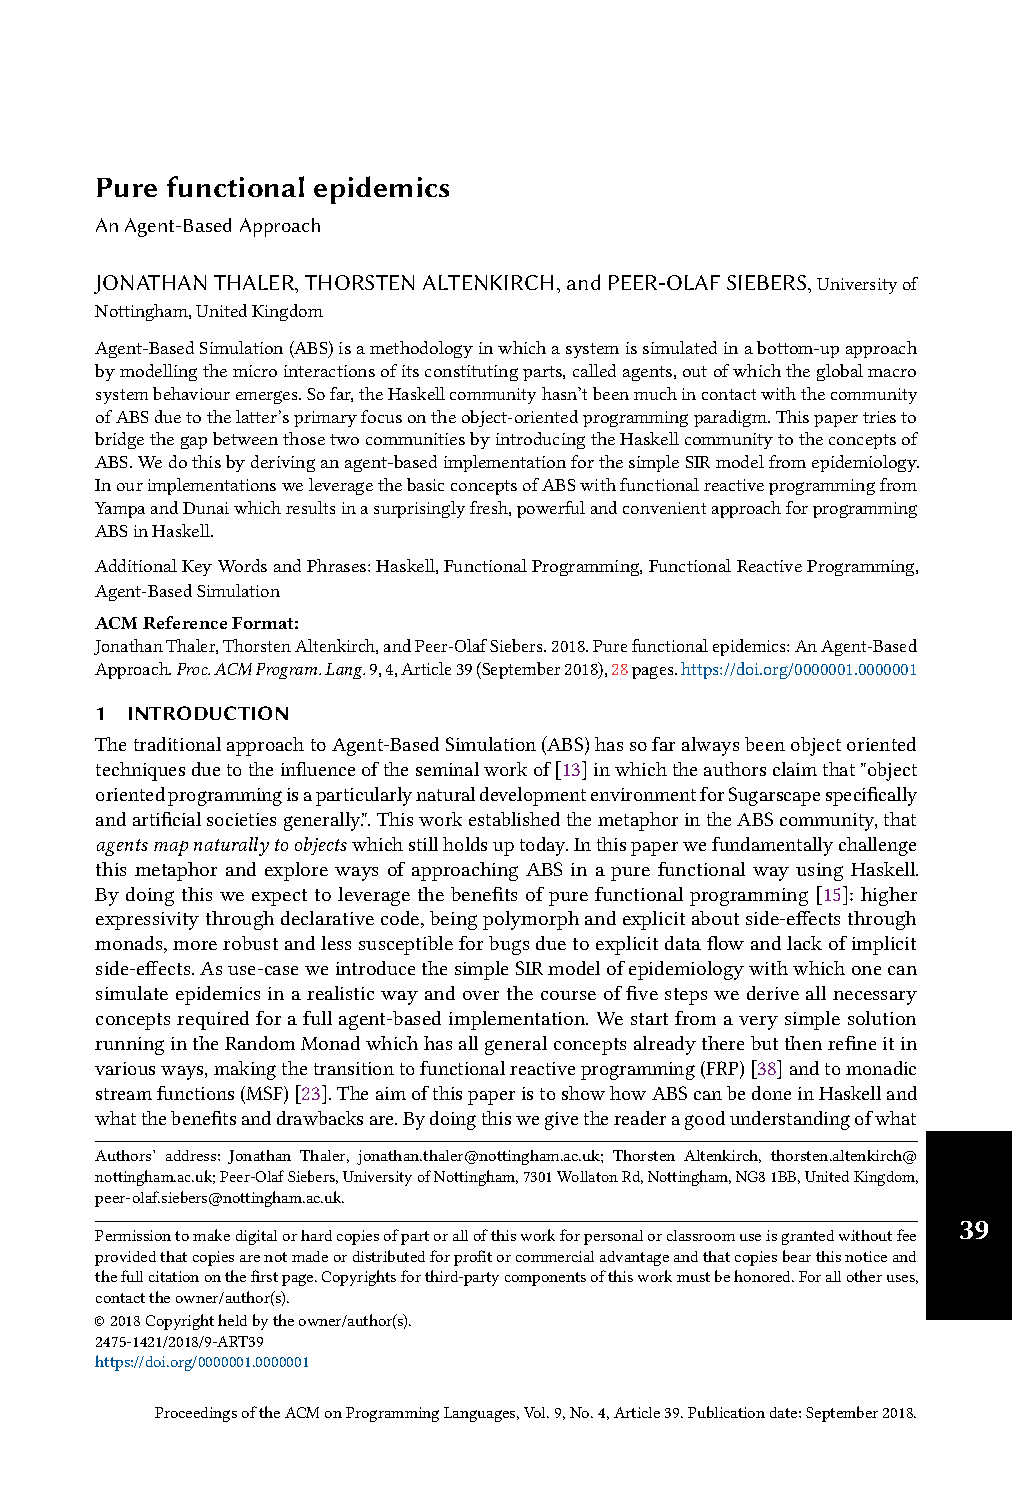
\includepdf[pages=-]{./pdf/pfe.pdf}

% NOTE: keep it out to the submission for the reviewers
%\chapter{Questions \& Answers}
\label{chap:qa}

TODO: update and adopt to 2nd year

In this chapter I give answers to anticipated questions and objections about my research direction and vision of doing pure functional ABS \footnote{They are not always posed in a dead-serious way but as it is a quite controversial topic - ABS should be done object-orientated after all huh? - I think it is appropriate. Also some objections were raised in exactly this way.}.

\paragraph{So you had this hypothesis, that pure functional programming and dependent types lead to simulation software which is more likely correct and is easier to verify and validate, right from the beginning?}
Not at all. I even had no deep knowledge of functional programming at the start of my PhD, I've just worked through the 1st edition of Grahams book "Programming in Haskell" and that's it. I had no clear understanding of purity, side-effects and Monads and I didn't know a bit about functional reactive programming. I knew that something like Dependent Types exist because Thorsten (2nd Supervisor) has sent me an email before the start of my PhD in which he pointed at Agda, so I started reading a bit about intuitionistic / constructivistic math, tried out a little bit of Agda but quickly gave up because it was way too far away (without really having mastered pure functional programming in Haskell, I believe it is nearly impossible / too difficult / makes no sense going into dependent types).
So in the beginning there was pure \textit{curiosity} about functional programming in combination with ABS because I knew nothing of FP at all and wanted to understand it (after getting bored by OO) and applying FP to ABS seemed so crazy (because everyone claims OO to be 'natural' for it) that it must be an extremely interesting challenge. I guess this is very often the case with research: there is 'just' curiosity in the beginning and then during the research process a hypothesis falls into place.


\chapter{Thesis Structure}
\label{app:thesis_struct}

TODO: find the story of my PhD thesis and connect it to my publication plan. 
TODO: story e.g. "We need functional programming to reduce the potential sources of bugs and introducing bugs harder, resulting in software which is more likely to be correct. Additionally by using dependent types we can narrow the gap between model specification and implementation even further, resulting in software which is even more likely to be correct. Further, additional benefits fall into place: purity leads to guaranteed reproducibility at compile-time, software transactional memory can be utilised to scale up to massively parallel and we have property-based testing at hand which puts the focus on specification testing rather than testing operational details".

This appendix gives a first draft of the structure outline of the thesis which I plan on start writing in April 2019. I aim for a flat structure which emphasises a strong narrative. The order of writing will be: Methodology, Proof-Of-Concept chapters, Literature Review, Discussion, Conclusions, Introduction, Abstract.
%
%line of argument
%1. established methods need extensive unit-testing for establishing correctness of software, which only increases the likelihood of correctness and doesnt guarantee it because they are inherent dynamic, testing run-time behaviour, because of the different type system.
%2. functional programming as in haskell has a strong static type system which allows to shift much much more guarantees towards static, compile-time, making many run-time tests obsolete and can guarantee a few things already at compile-time which makes tests to cover that completely obsolete
%3. dependent types can push these guarantees even further and theoretically should allow to express guarantees at compile-time to an arbitrary complex level which in theory should allow us to abandon run-time testing of bugs altogether. This does not mean that we don't need any tests anymore, as will be outlined in the chapter on Verification \& Validation \ref{chap:v_and_v}.
%4. with shifting more towards compile-time guarantees we automatically gain more confidence into the correctness of our simulation and reduce the implementation overhead of writing tests for those cases. Also some properties are simply not testable with run-time tests e.g. that some property holds forever - this is only possible to guarantee by looking at the code directly (where functional programming shines) or expressing it through compile-time guarantees. 
%5. correct by construction: narrowing the gap between model specification and implementation 
%6. Impedance Mismatch: ABS is constructive / generative in nature but the nature of the test-driven development process is deductive. is this a problem? Think of it more deeply


\section{Introduction}
This chapter is the introduction to the thesis and motivates it and describes the aim and scope of the Ph.D. Further it states the hypotheses and contributions.
\begin{itemize}
	\item Main Argument: Defining the problem, motivation, aim and scope of the Ph.D.
	\item Hypotheses: Precisely stating the hypotheses which will form the points of reference for the whole research.
	\item Contributions: Precisely list the contribution to knowledge this Ph.D. makes and list all papers which were written (and published) during this Ph.D.
\end{itemize}

\section{Literature Review}
This chapter discusses background and related work by presenting the relevant literature 

\section{Methodology}
This chapter introduces the methodology, used in the experimental chapters:

\begin{itemize}
	\item Defining and introducing Agent-Based Simulation (ABS) (History, ABS vs. MAS, examples, event- vs. time-driven).
	\item Introduce established implementation approaches to ABS (Frameworks: NetLogo, Anylogic, Libraries: RePast, DesmoJ, Programming: Java, Python, Correctness: ad-hoc, manual testing, test-driven development)
	\item Introduction Verification \& Validation (V \& V in the context of ABS).
	\item Introduction to functional Programming in Haskell (functions, types, recursion, algebraic data-types, higher-order functions, continuations, Define and explain side-effects and purity: monads, different types of effects, explain IO and that it is of fundamental importance to avoid it in our research).
	\item Introduction to dependent types (Example, Equality as Type, Philosophical Foundations: Constructive mathematics)
\end{itemize}

\section{Case Studies}
Presents case studies which are the main contribution of this Ph.D. which support our hypothesis. Each section is structured by Intro, Methods, Experiment, Analysis.

\subsection{Case Study 1: Testing and Verification}
This chapter describes how testing \& verification works in pure functional ABS.
%\begin{itemize}
%	\item Testing in functional programming
%	\item Strong Static Types rule out some classes of bugs and make some tests obsolete.
%	\item Property-Based testing: QuickCheck.
%	\item Using Property-Based testing in ABS for specification testing.
%	\item Reasoning about code
%\end{itemize}

\subsection{Case Study 2: Going Large-Scale}
This chapter discusses how pure functional ABS can go large-scale using STM. Further it is the central chapter, discussing various types of agent-agent and agent-environment interactions

%\subsubsection{Agent-Agent Interactions}
%This is the central problem of the FP approach as basically the agent-interactions define the level of abstractions over the agents. Unfortunately this is easier and more elegant in object-oriented programming. Still, by using a strong static type system we are more explicit about agent-interactions and we can have advantages which OOP doesn't have. Also we show that there are multiple different kinds of agent-interactions, depending on whether it is a time- or event-driven ABS.
%There is still much work to be done for this thesis chapter, we need to distinguish between:
%
%\begin{itemize}
%	\item Asynchronous Interaction: the flow is one-directional and does not need a listener on the other side and not a synchronous reply. The mechanism depends strongly on the type of ABS: time- or event-driven and pure or concurrent. Examples are the pure feedback in the Yampa SIR implementation, pure Data-Flow in the Yampa implementation, pure agent transactions, pure events, STM Event, STM message-boxes.
%	\item Synchronous Interactions: the flow is bi-directional and needs a listener on the other side to engage in a synchronous interaction without time-delay. We have only touched on prototyping this but need to go deeper for the final thesis. In Haskell we could build on the pure event driven approach we have implemented already in Step7\_EventDriven but we need to extend it towards an explicit synchronous mechanism. Also we need to show how we can do this in STM but there its gonna be very tricky because all agents act conceptually at the same time.
%\end{itemize}

\subsection{Case Study 3: Dependent Types}
This chapter gives an in-depth discussion on how dependent types can be made of use in pure functional ABS.

\section{Discussion}
This chapter re-visits the hypotheses and puts them into perspective of the contributions.

\section{Conclusions}
This chapter draws conclusions to the main hypothesis and outlines future research.

\section{Appendices}
Datasets, lengthy code, additional proofs.


\end{appendices}

\end{document}
